\documentclass[xcolor=table]{beamer}
\usetheme{ALUF}

\usepackage[utf8]{inputenc}
% \usepackage{palatino}
% \usepackage[T1]{fontenc}
\usepackage{lmodern}
\usepackage[protrusion=true,expansion=true,tracking=true,kerning=true]{microtype}
\usepackage{graphicx}
\usepackage[utf8]{inputenc}
\usepackage{color}
\usepackage{textcomp}
\usepackage{charter}
\usepackage[T1]{fontenc}
\usepackage[frenchb]{babel}
\usepackage{caption}
\usepackage{pdfpages}
\usepackage{array}
\usepackage{supertabular}
\usepackage{hyperref}
\usepackage{fancyhdr} 
\usepackage{eurosym}
\usepackage{multirow}
\usepackage{parallel}
\usepackage{booktabs}
\usepackage{tikz}
\usetikzlibrary{arrows, decorations.markings}

\newcommand{\tabitem}{\par\hspace*{\labelsep}\textbullet\hspace*{\labelsep}}

%Permet de faire des listes dans les tableaux
\makeatletter
\newcolumntype{e}[1]{%--- Enumerated cells ---
   >{\minipage[b]{\linewidth}%
     \NoHyper%                Hyperref adds a vertical space
     \let\\\tabularnewline
     \enumerate
        \addtolength{\rightskip}{0pt plus 50pt}% for raggedright
        \setlength{\itemsep}{-\parsep}}%
   p{#1}%
   <{\@finalstrut\@arstrutbox\endenumerate
     \endNoHyper
     \endminipage}}

\newcolumntype{i}[1]{%--- Itemized cells ---
   >{\minipage[b]{\linewidth}%
        \let\\\tabularnewline
        \itemize
           \addtolength{\rightskip}{0pt plus 50pt}%
           \setlength{\itemsep}{-\parsep}}%
   p{#1}%
   <{\@finalstrut\@arstrutbox\enditemize\endminipage}}

\AtBeginDocument{%
    \@ifpackageloaded{hyperref}{}%
        {\let\NoHyper\relax\let\endNoHyper\relax}}
\makeatother

\defbeamertemplate*{title page}{supdefault}[1][]
{
  \vbox{}
  \vfill
  \begingroup
    \centering
    \begin{beamercolorbox}[rounded=true, shadow=true,sep=8pt,center,#1]{title}
      \usebeamerfont{title}\inserttitle\par%
      \ifx\insertsubtitle\@empty\relax%
      \else%
        \vskip0.25em%
        {\usebeamerfont{subtitle}\usebeamercolor[fg]{subtitle}\insertsubtitle\par}%
      \fi%     
    \end{beamercolorbox}%
    \vskip1em\par
    \begin{beamercolorbox}[sep=8pt,center,#1]{author}
      \usebeamerfont{author}\insertauthor
    \end{beamercolorbox}
    \begin{beamercolorbox}[sep=8pt,center,#1]{institute}
      \usebeamerfont{institute}\insertinstitute
    \end{beamercolorbox}
    \begin{beamercolorbox}[sep=8pt,center,#1]{date}
      \usebeamerfont{date}\insertdate
    \end{beamercolorbox}\vskip0.5em
    {\usebeamercolor[fg]{titlegraphic}\inserttitlegraphic\par}
  \endgroup
  \vfill
}
%\setbeamertemplate{title page}[supdefault][colsep=-4bp,rounded=true,shadow=true]\makeatother

%Style de flèche pour le schéma
\tikzstyle{vecArrow} = [thick, decoration={markings,mark=at position
   1 with {\arrow[semithick]{open triangle 60}}},
   double distance=1.4pt, shorten >= 5.5pt,
   preaction = {decorate},
   postaction = {draw,line width=1.4pt, white,shorten >= 4.5pt}]
\tikzstyle{innerWhite} = [semithick, white,line width=1.4pt, shorten >= 4.5pt]

%Définition des variables
\title{24 heures de l'INSA - 44\up{ème} édition}
\subtitle{18 - 20 mai 2018}
\author{Formation Grands Rassemblements}
\date{23 avril 2018}
\institute{Arthur Saunier - 06 25 53 25 79 \\Valentin Godrie - 07 52 62 04 69\\Léo Mouyna - 06 24 30 26 53}

\begin{document}

\begingroup
\makeatletter
\setlength{\hoffset}{-.5\beamer@sidebarwidth}
\makeatother
\begin{frame}[plain]
     \titlepage
\end{frame}
\endgroup

\begin{frame}% [plain,t]
	\frametitle{Ordre du jour}
\tableofcontents
\end{frame}

%=============================================================================================

%========================================
%PRESENTATION DE LA MANIFESTATION
%========================================

\section{Présentation de la manifestation}

\begin{frame}

\centering\Huge{\textbf{Présentation de la manifestation}}

\end{frame}

\begin{frame}

\frametitle{Généralités}

\setlength{\tabcolsep}{2pt}
\setlength{\extrarowheight}{.75ex}
\begin{tabular}{cccc}
\hline
\multicolumn{4}{|c|}{\centering\Large\textbf{44\up{ème} édition - 18, 19 et 20 mai 2018}}\\
\hline
\\
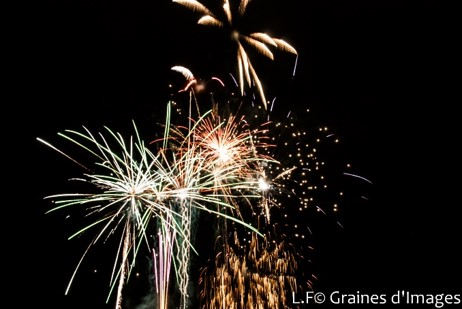
\includegraphics[height=.2\textheight]{Images/Image1} & 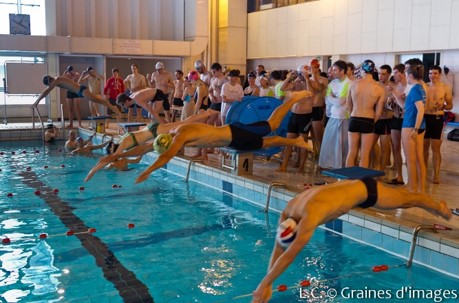
\includegraphics[height=.2\textheight]{Images/Image2} & 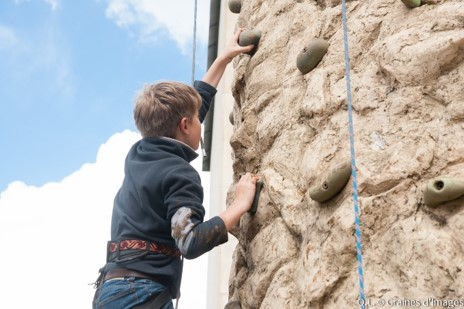
\includegraphics[height=.2\textheight]{Images/Image3} & 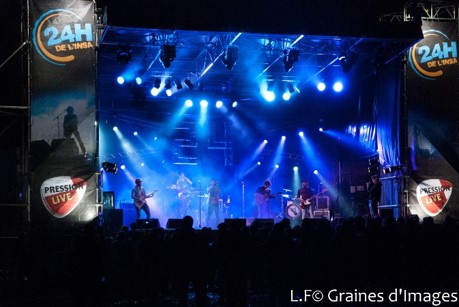
\includegraphics[height=.2\textheight]{Images/Image4}\\
\\
\multicolumn{4}{l}{\tabitem 24 heures de courses}\\
\multicolumn{4}{l}{\tabitem 3 soirs de concerts}\\
\multicolumn{4}{l}{\tabitem 2 journées d'animations gratuites}\\
\multicolumn{4}{l}{\tabitem Environ 30 000 personnes sur 3 jours}\\

\end{tabular}

\end{frame}

\begin{frame}

\frametitle{Les 24 heures en quelques chiffres}

\begin{itemize}
\item \textbf{50} organisateurs toute l'année
\item \textbf{300} bénévoles le week-end
\item \textbf{9000} personnes par soirée (2017)
\item \textbf{30 000} personnes attendues sur le week-end
\end{itemize}

\end{frame}

\begin{frame}

\frametitle{Plan général du site}

\centering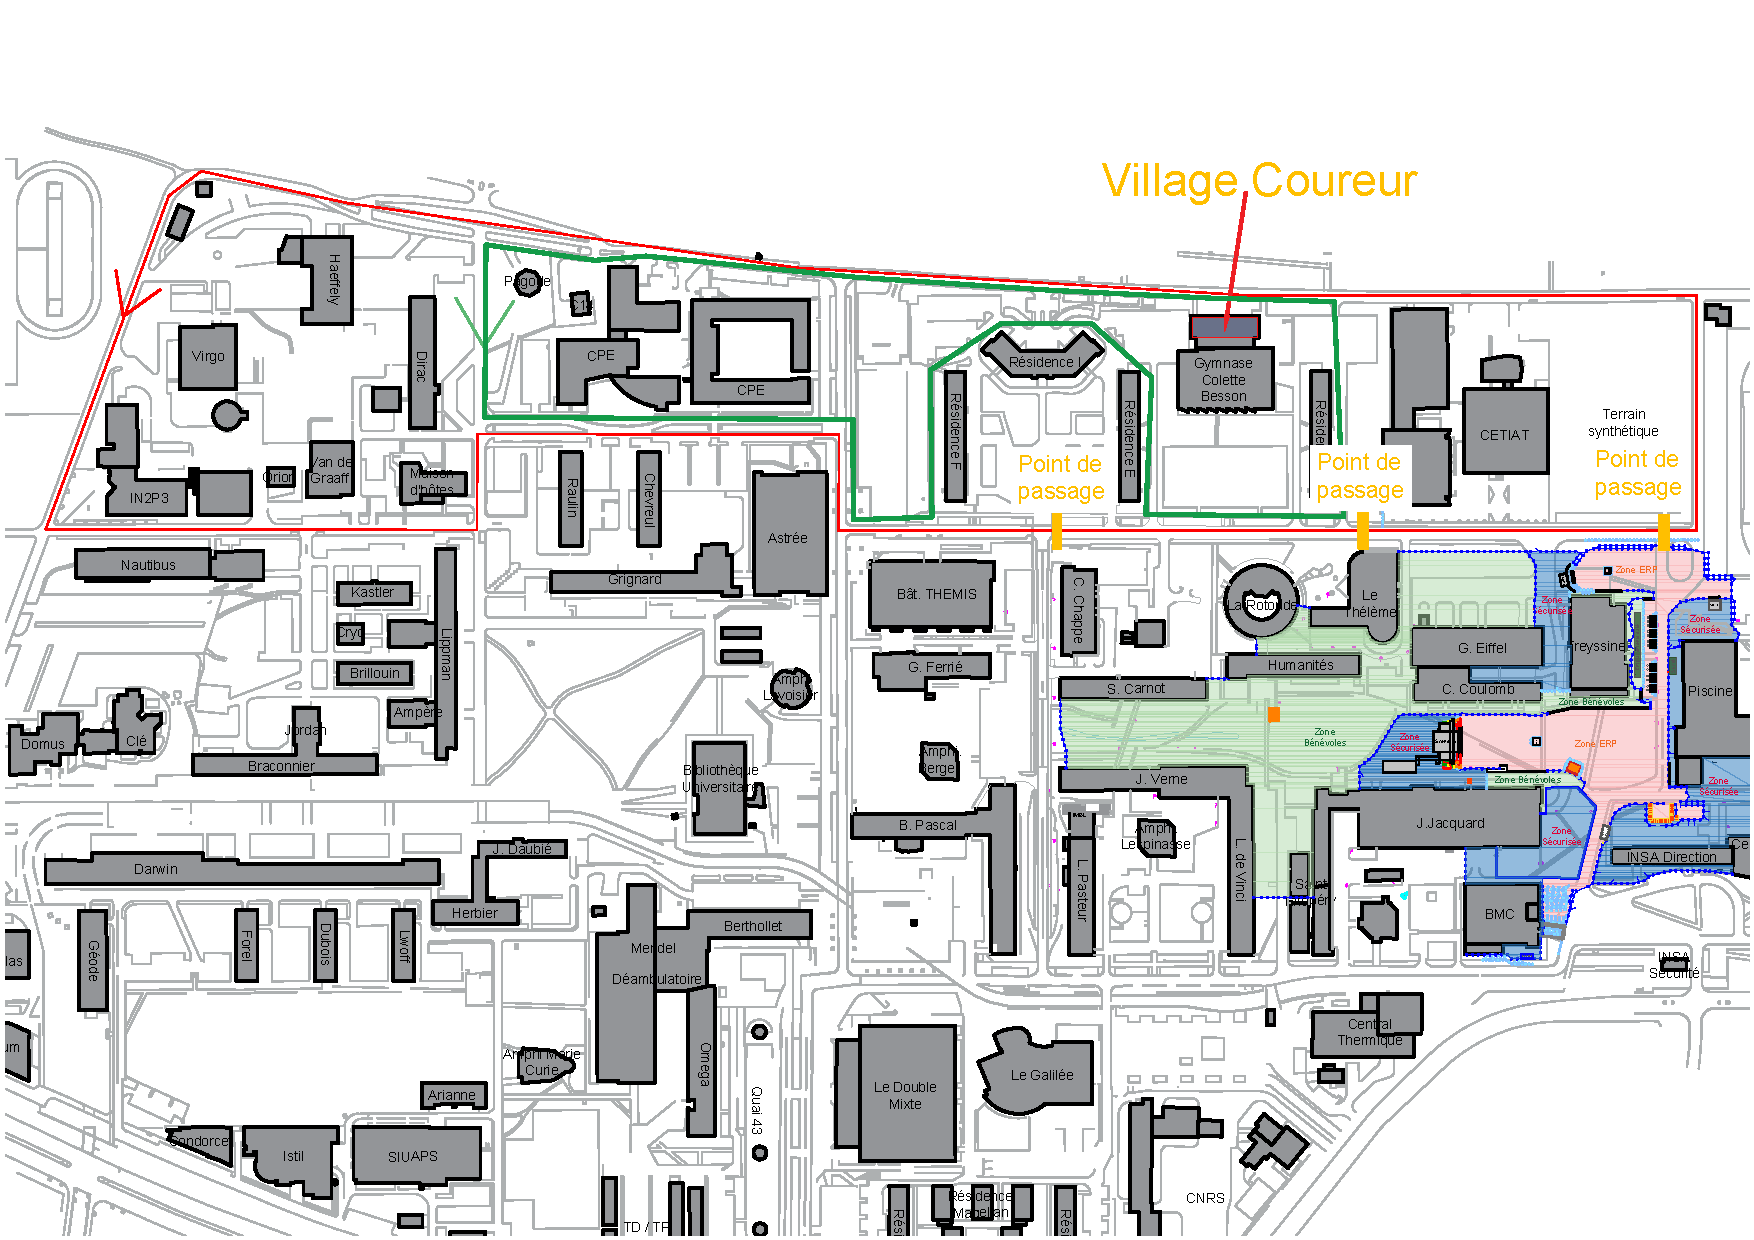
\includegraphics[height=.8\textheight, trim=150 70 0 0,clip]{Exports/Plan_24h_44eme-Parcours_courses}

\end{frame}

\begin{frame}

\frametitle{Organisation}

\centering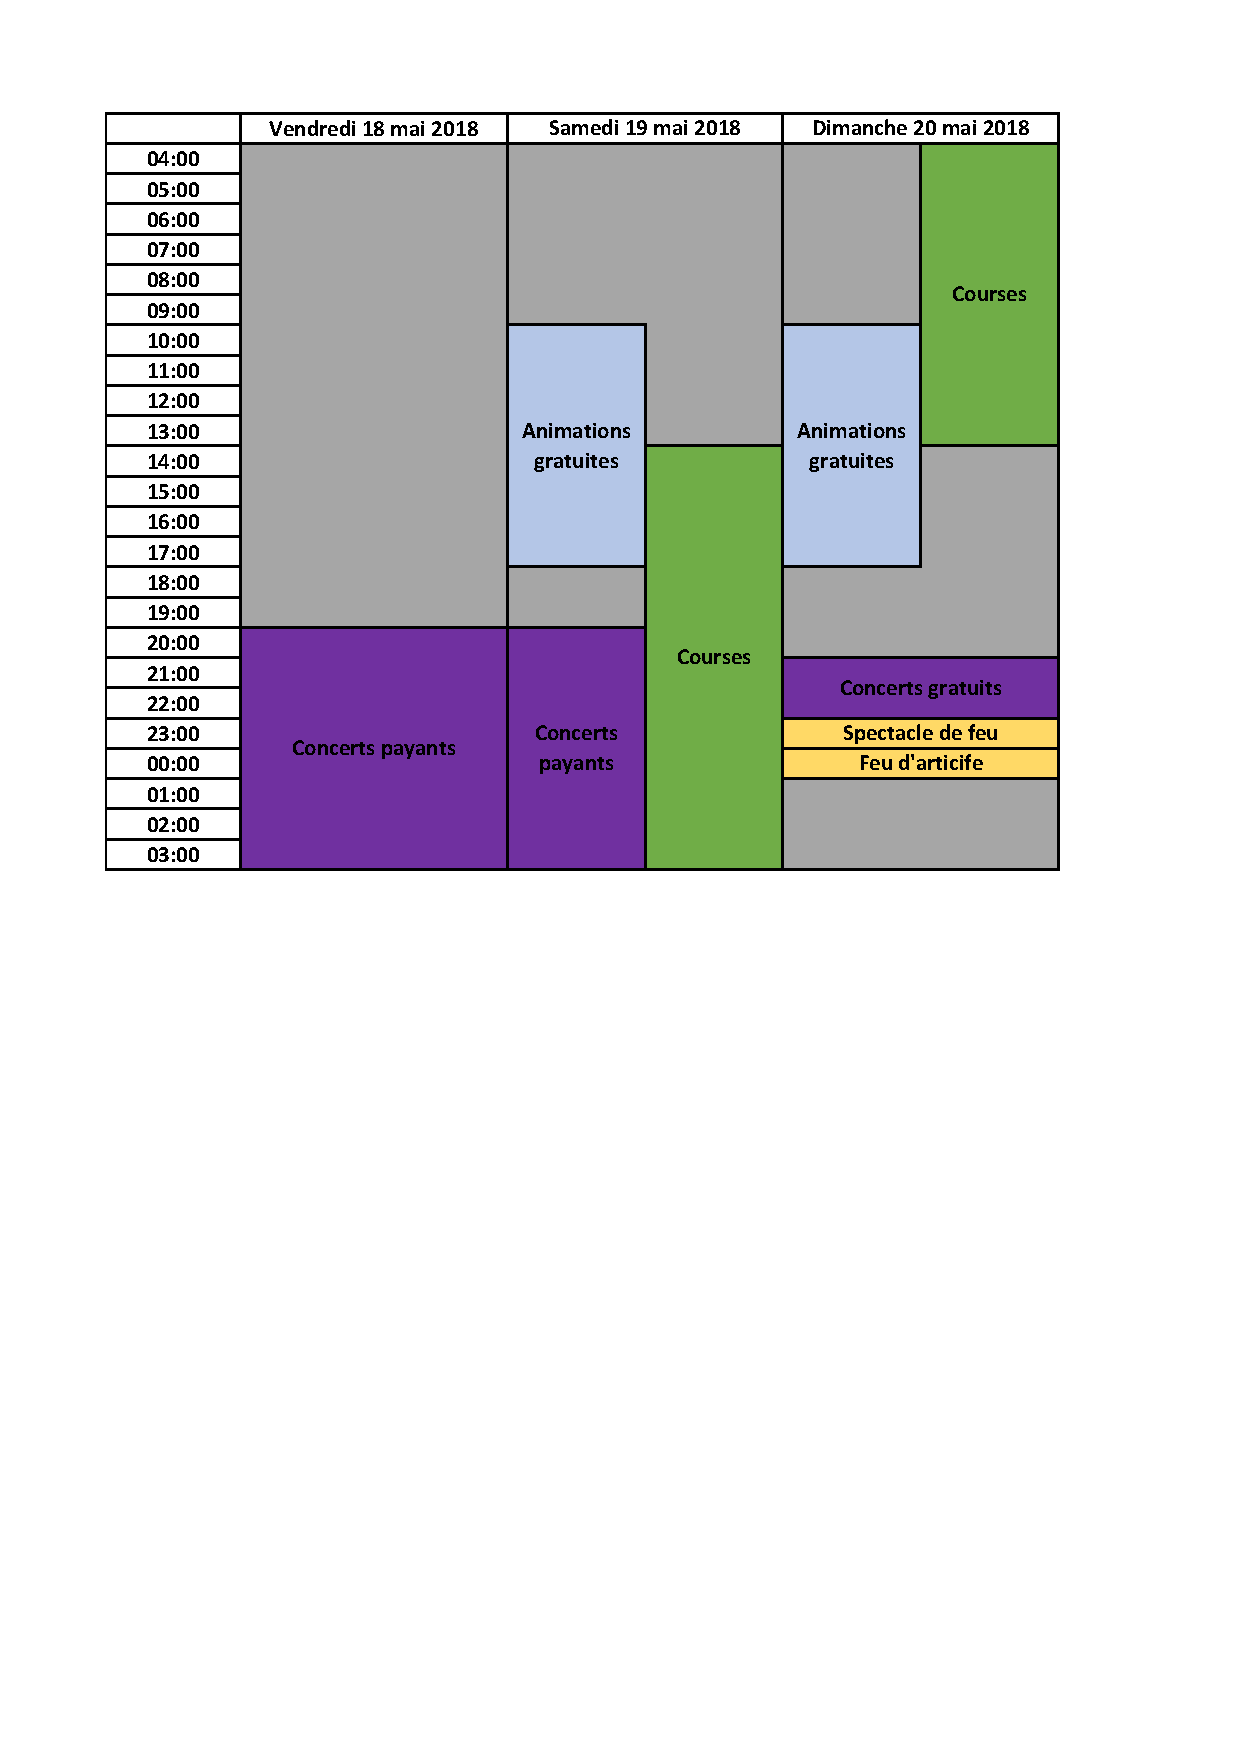
\includegraphics[width=\textwidth]{Images/Timeline}

\end{frame}

%========================================
%BILAN DE L'EDITION 2017
%========================================

\section{Bilan 2017}

\begin{frame}

\centering\Huge{\textbf{Bilan 2017}}

\end{frame}

\begin{frame}

\frametitle{Nouvelles dispositions}
\begin{itemize}
\item\textbf{Nouveau dispositif de fermeture à la circulation}

$\rightarrow$ Aucun forçage du dispositif pendant les périodes concernées (20h-5h)

\item\textbf{Ajout de silo à verre aux entrées}

$\rightarrow$ Moins de verre présent autour de cette zone

\item\textbf{Augmentation et répartition des effectifs d'AS en journée}

$\rightarrow$ Aucun incident notable pendant les deux journées d'animations
\end{itemize}
\end{frame}

\begin{frame}

\frametitle{Remarques générales}
\begin{itemize}
\item Public majoritairement étudiant en soirée
\item Très peu de problèmes rencontrés sur l'ensemble du week-end
\item Plusieurs pickpockets arrêtés par la Police, une cinquantaine de téléphones récupérés
\item Quelques points de passage forcés par des véhicules en journée
\item Quelques collisions cyclistes/spectateurs
\end{itemize}
\end{frame}

\begin{frame}

\frametitle{Affluence}
\rowcolors[\hline]{2}{blue!30}{blue!10}
\begin{tabular}{|l|c|c|c|c|}
\hline
\rowcolor{blue!50} &\bf2015&\bf2016&\bf2017&\bf\parbox[c]{1.7cm}{\centering{Variation}\\2016/2017}\\
\hline
Vendredi soir  & 8700 & 8400 & 7600 & -10\%\\
\hline
Samedi soir  & 8000 & 9650 & 8400 & -13\%\\
\hline
Dimanche soir & 900 & 1600 & 1000 & -60\%\\
\hline
Total soirées & 17 600 & 19 650 & 17 000 & -13\%\\
\hline
Samedi journée & 5000 & 4000 & 5000 & +25\%\\
\hline
Dimanche journée & 5000 & 5000 & 5000 & =\\
\hline
Total journées  & 10 000 & 9000 & 10 000 & +11\%\\
\hline
Total festival  & 27 600 & 28 650 & 27 000 & -6\%\\
\hline

\end{tabular}

\end{frame}

\begin{frame}

\frametitle{Interventions}

\rowcolors[\hline]{2}{blue!30}{blue!10}
\begin{tabular}{|l|c|c|c|c|}
\hline
\rowcolor{blue!50} &\bf2015&\bf2016&\bf2017&\bf\parbox[c]{1.7cm}{\centering{Variation}\\2016/2017}\\
\hline
Croix-Rouge & 101 & 68 & 69 & =\\
\hline
STAFF Sécurité & 14 & 18 & 5 & -72\%\\
\hline
\end{tabular}

\end{frame}

\begin{frame}

\frametitle{Nouveautés 2018}
\framesubtitle{Prise en compte du bilan 2017}

\begin{itemize}
\item Modification des emplacements du PCO et PCS
\item Second périmètre anti-bélier
\item Modification des effectifs aux points d'accès
\item Regroupement des toilettes sur une unique zone
\item Changement d'infrastructures scéniques
\item Nouvelle animation à sensation forte : la tyrolienne
\end{itemize}

\end{frame}

%========================================
%DISPOSITIF DE SECURITE
%========================================

\section{Dispositif de sécurité}

\begin{frame}

\centering\Huge{\textbf{Dispositif de sécurité}}

\end{frame}

\begin{frame}

\frametitle{Plans de situation}
\begin{Parallel}{.5\textwidth}{.5\textwidth}
\ParallelLText{\centering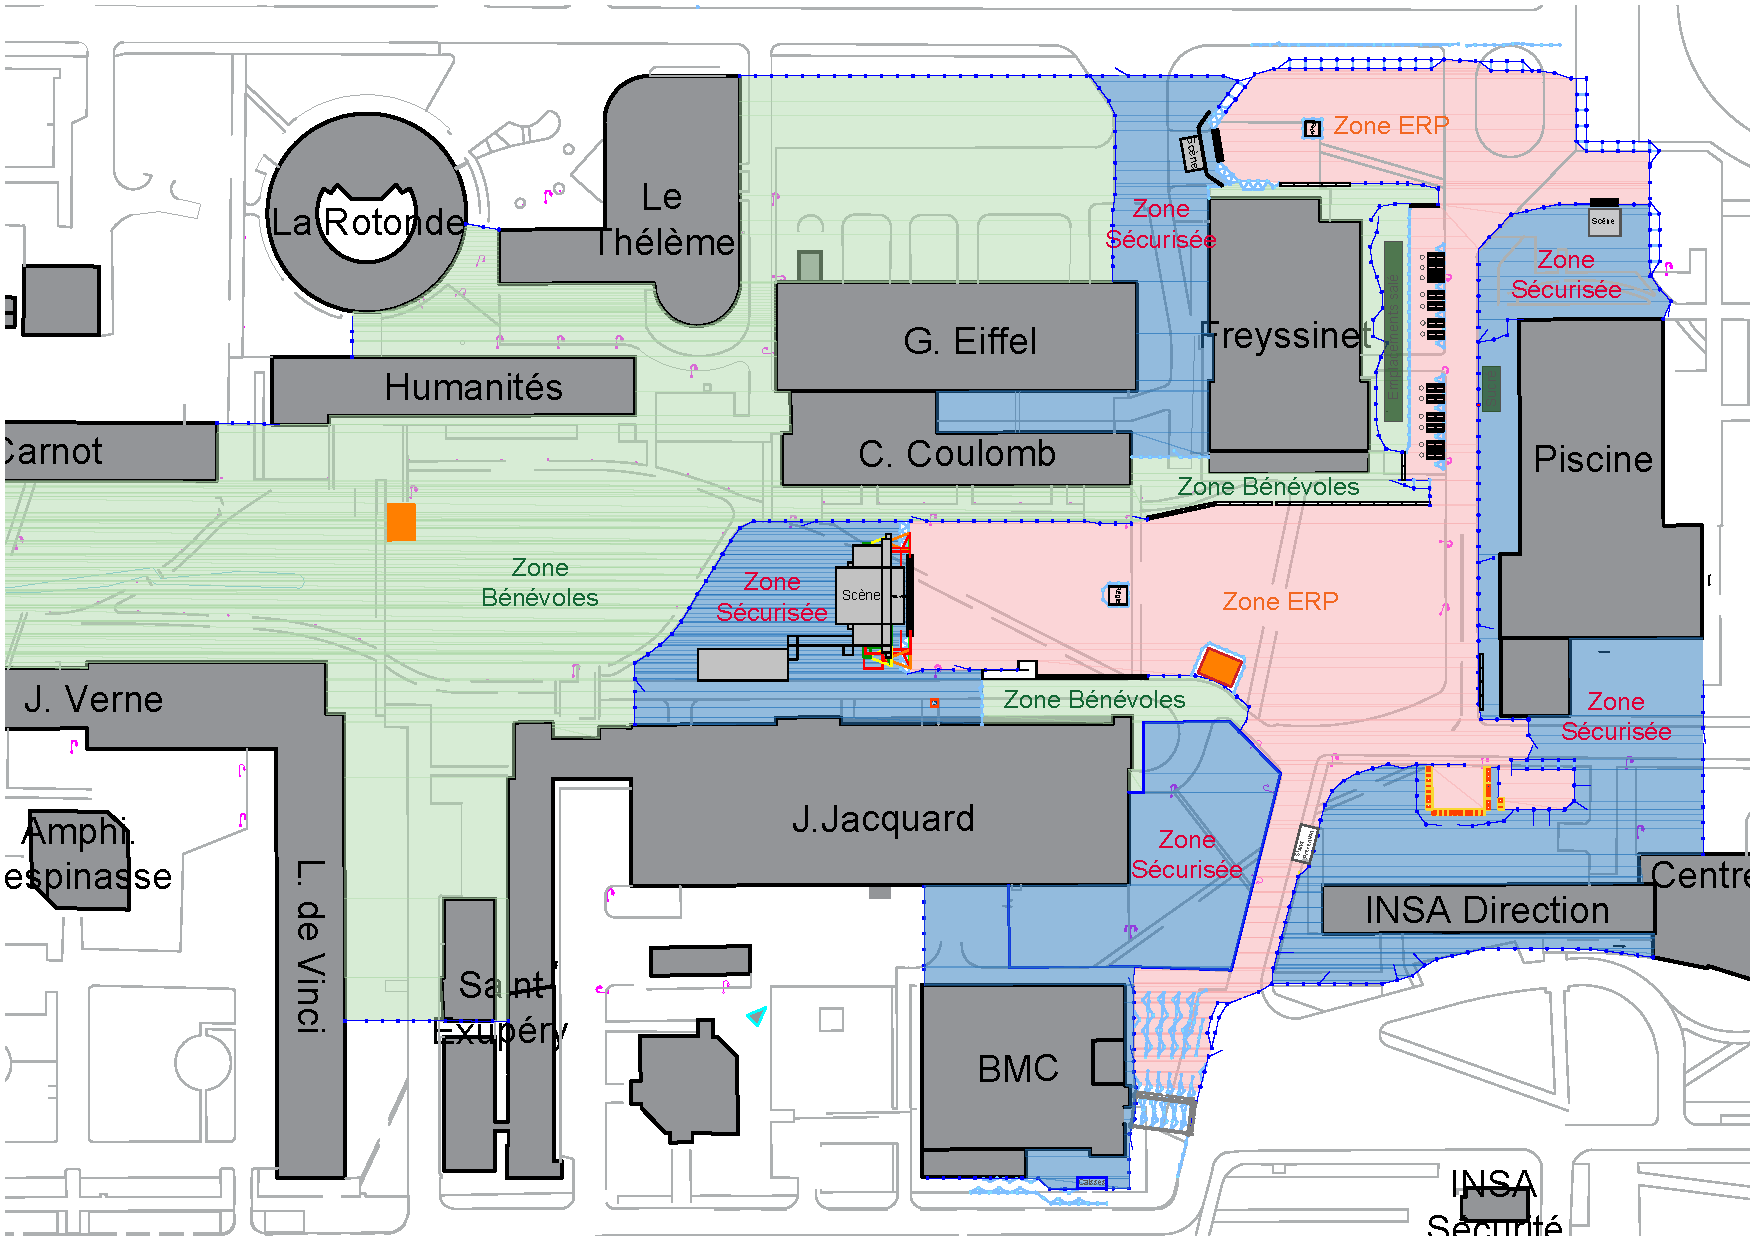
\includegraphics[height=.7\textheight, trim=300 20 0 0,clip]{Exports/Plan_24h_44eme-Plan_ERP}}
\ParallelRText{\centering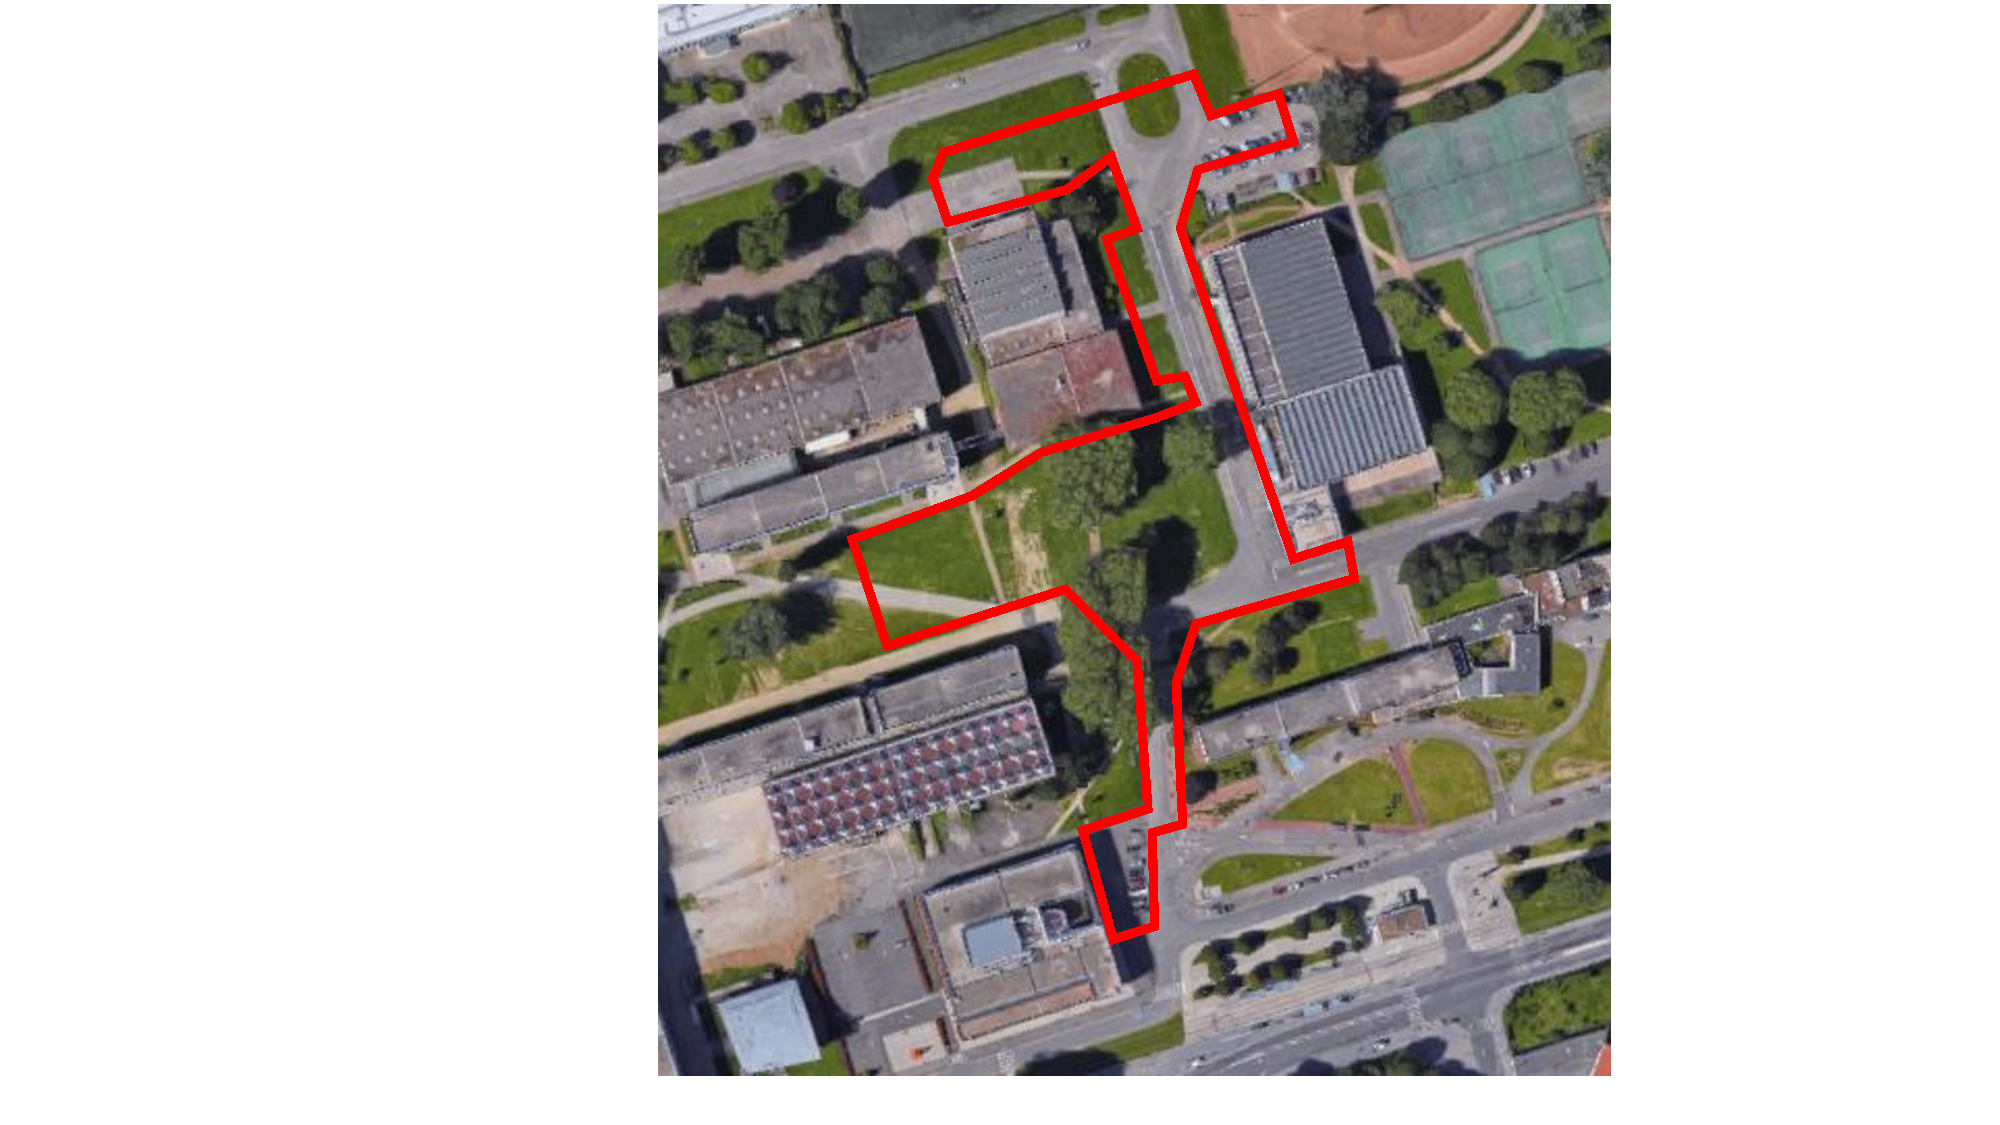
\includegraphics[height=.7\textheight, trim=0 0 0 0,clip]{Exports/ERP_vue_aerienne}}
\end{Parallel}

\end{frame}

\begin{frame}

\frametitle{Zone ERP}

\begin{tabular}{i{.5\textwidth} c}
\item Validation de la zone à \\ 30 900 personnes par la sous-commission ERP-IGH le 12 avril 2017
\vspace{0.5cm}
\item Exploitation à 10 000 personnes
\vspace{0.5cm}
\item Pas de commission cette année (modifications mineures seulement)
\vspace{.5cm}
& 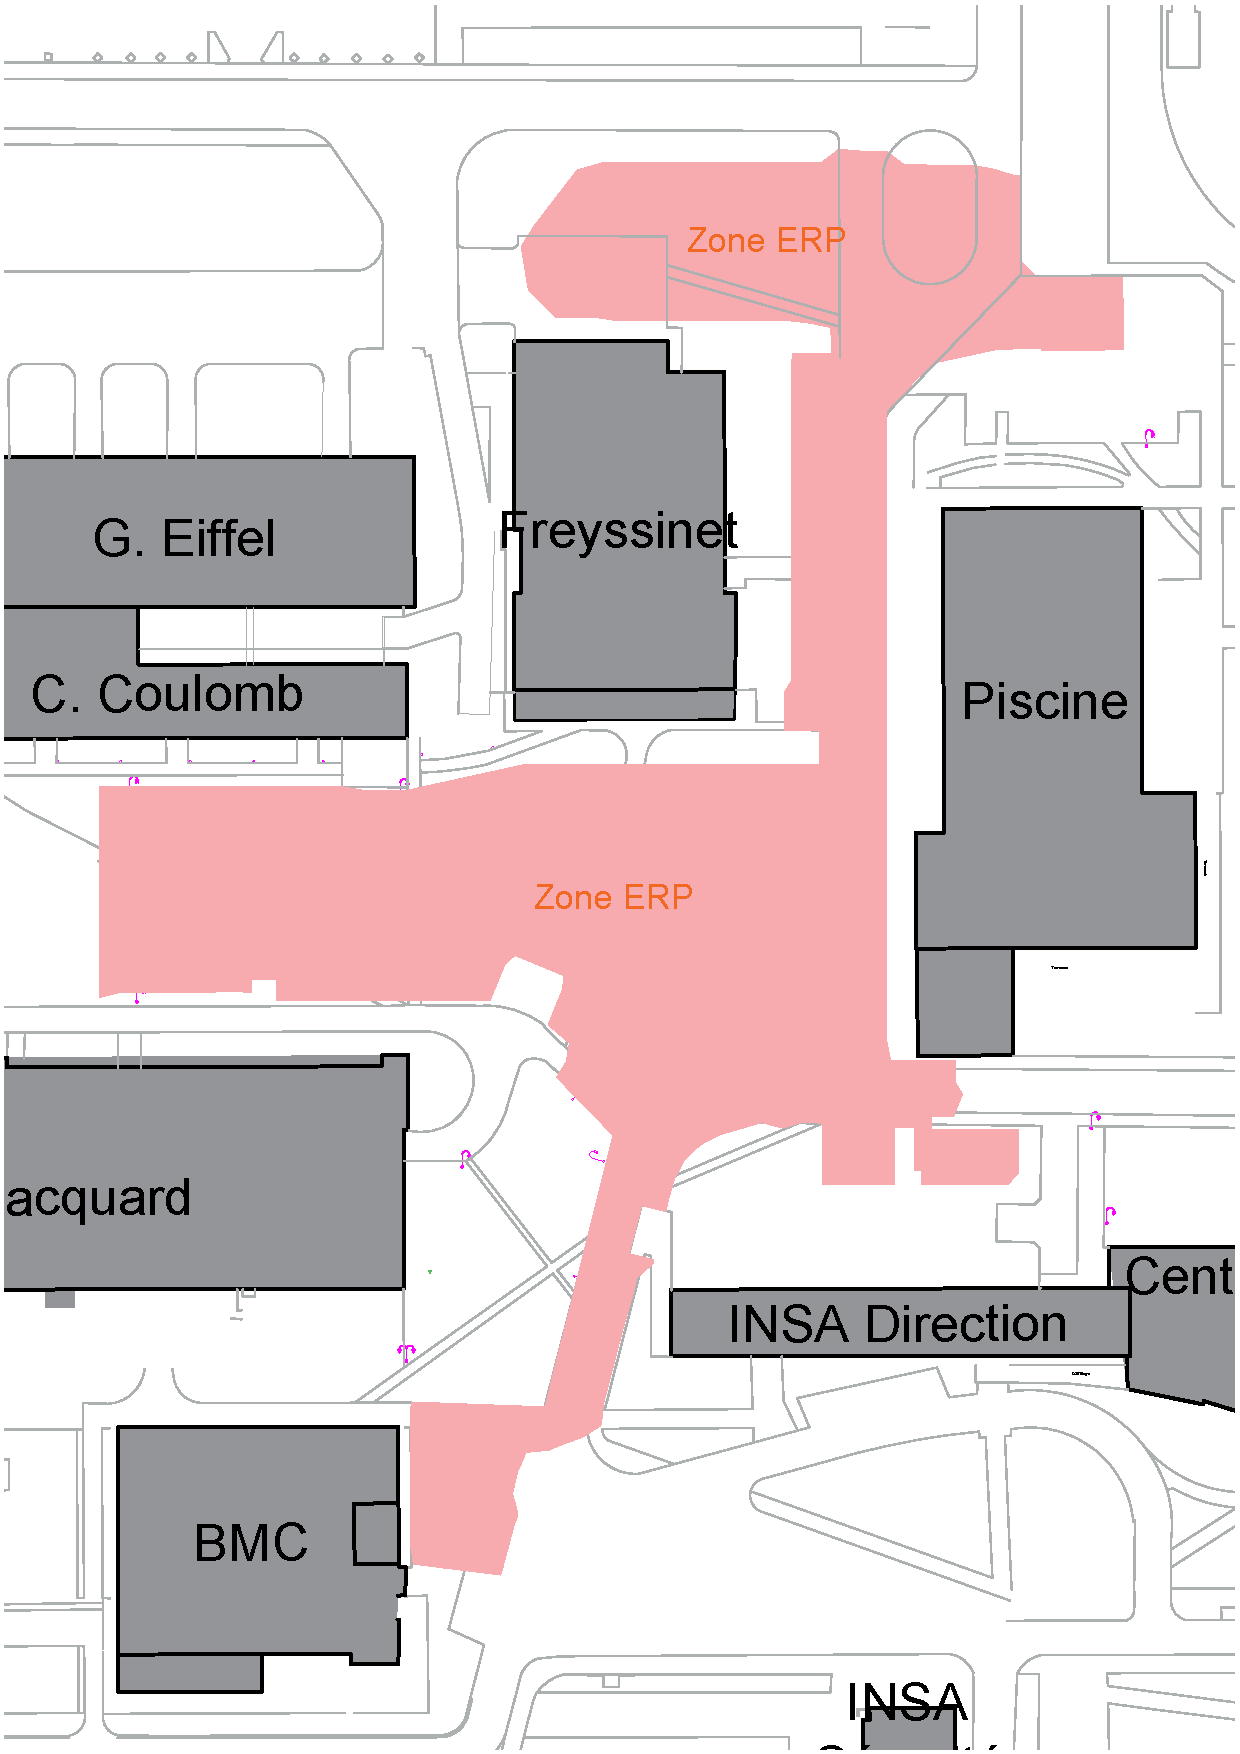
\includegraphics[height=.8\textheight, trim=0 0 0 0,clip]{Exports/Plan_24h_44eme-Plan_de_situation}\\
\end{tabular}

\end{frame}

\begin{frame}

\frametitle{Dégagements}
\begin{tabular}{i{.4\textwidth} c}
\item \textbf{13 sorties} pour un minimum de 13 imposées
\vspace{0.5cm}
\item \textbf{113 UP} pour un minimum de 103 imposées
\vspace{2cm}
& 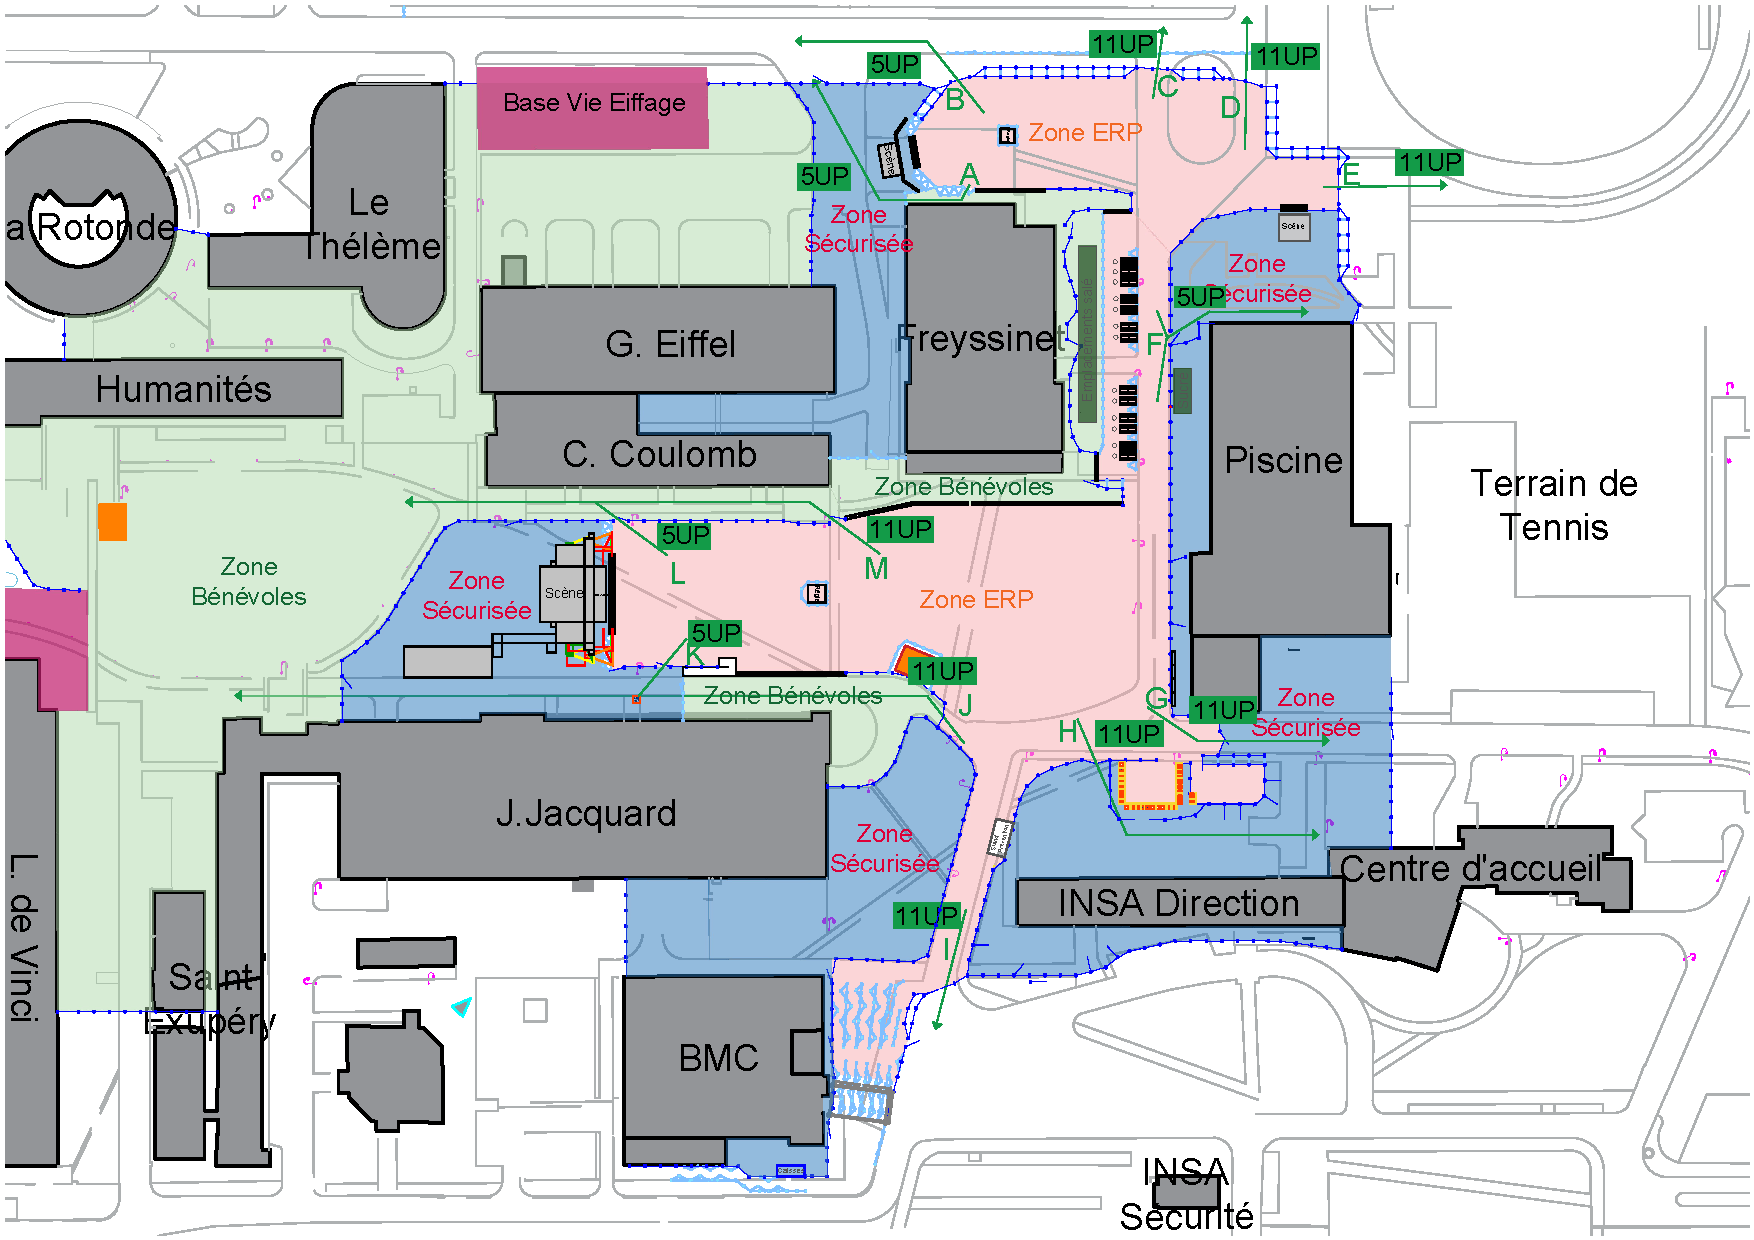
\includegraphics[width=.55\textwidth, trim=150 0 190 0,clip]{Exports/Plan_24h_44eme-IS}\\
\end{tabular}

\end{frame}

\begin{frame}

\frametitle{Voies pompiers}
\begin{tabular}{i{.4\textwidth} c}
\item \textbf{6 voies pompiers} autour de la zone ERP
\vspace{0.45cm}
\item \textbf{Agents de sûreté} préposés à l'ouverture en liaison avec le PC Sécurité
\vspace{0.45cm}
\item Procédures d'ouverture des accès rapide et fiables
& 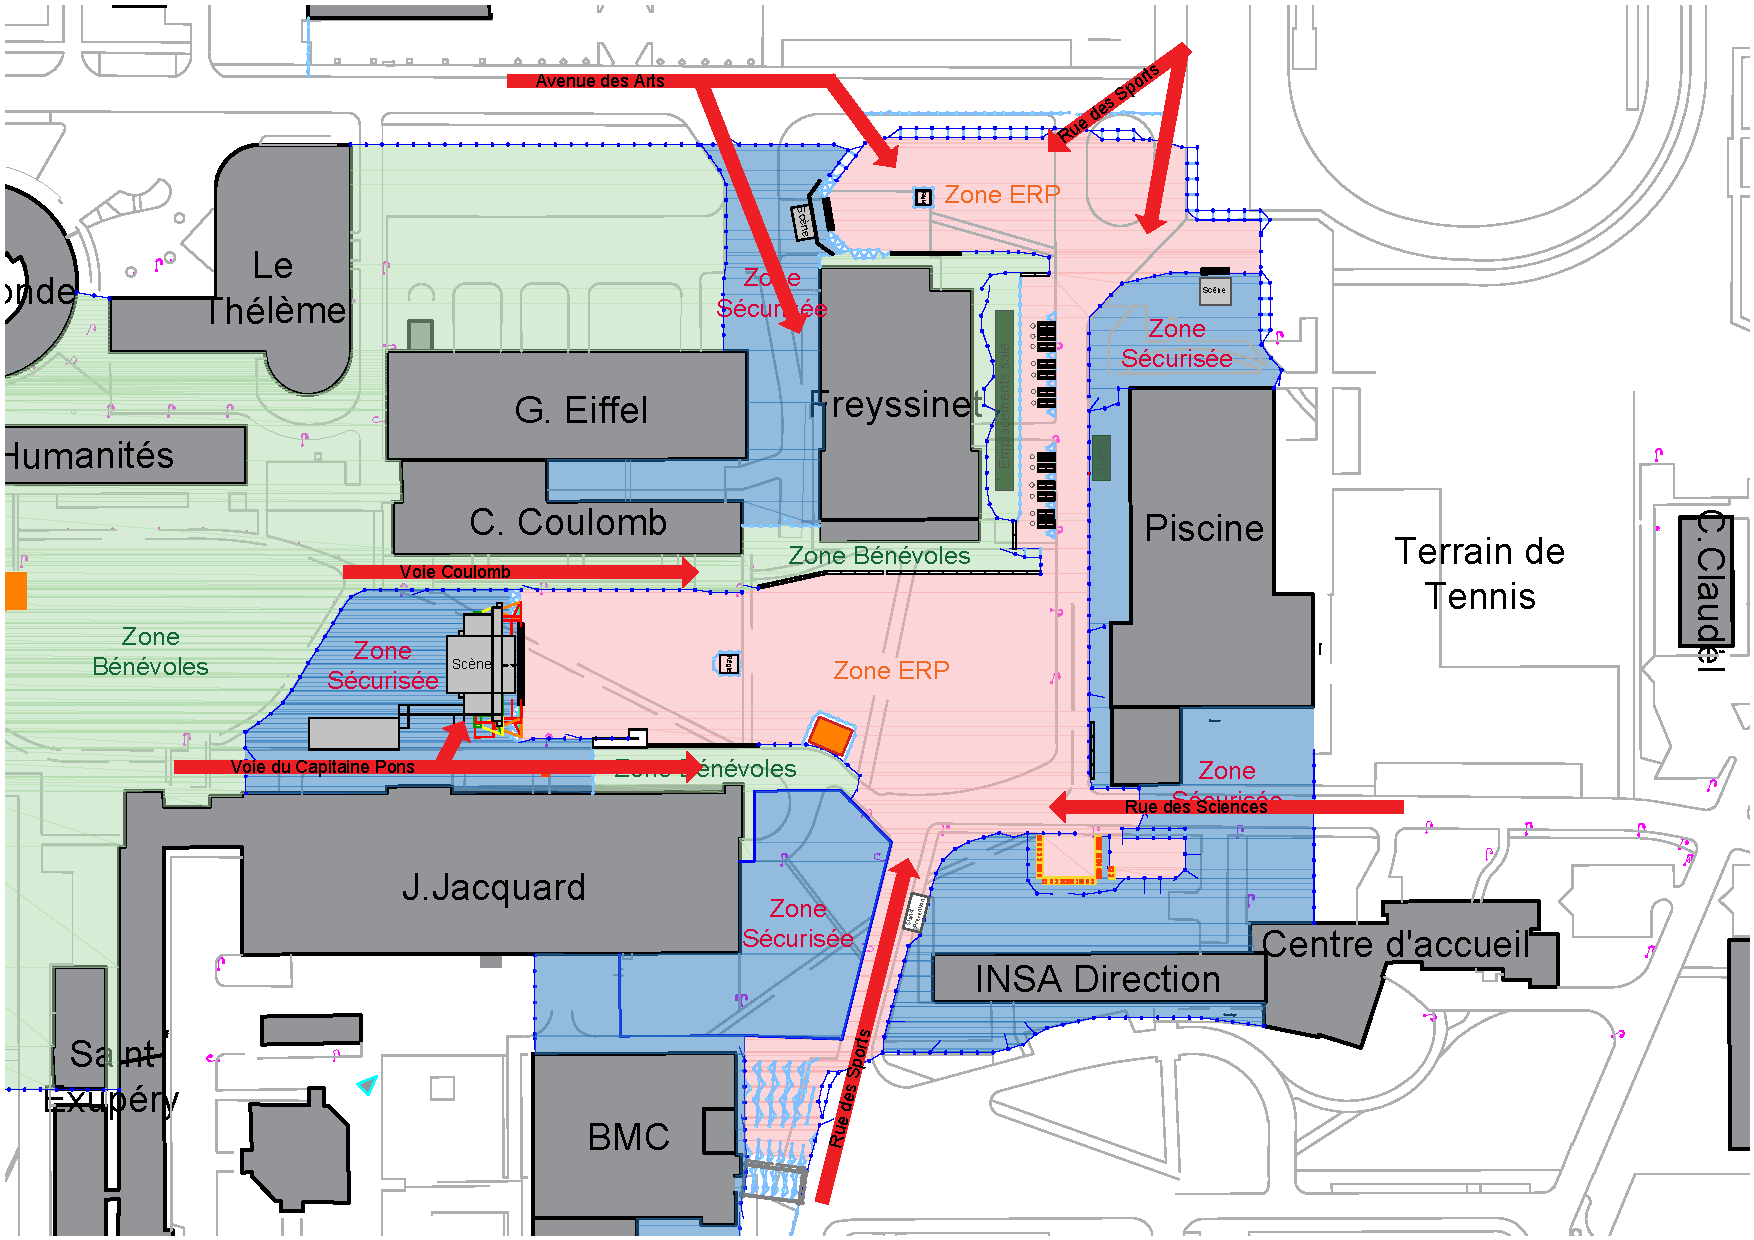
\includegraphics[width=.55\textwidth, trim=150 0 190 0,clip]{Exports/Plan_24h_44eme-Acces_Pompiers}\\
\end{tabular}

\end{frame}

\begin{frame}

\frametitle{Protection contre l'incendie}
\begin{tabular}{i{.4\textwidth} c}
\item \textbf{Agents de sécurité} incendie : 1 SSIAP 3, 2 SSIAP 2, 5 SSIAP 1
\vspace{0.3cm}
\item \textbf{28 exctinteurs} à disposition
\vspace{0.3cm}
\item \textbf{Sensibilisation} de 20 organisateurs à leur utilisation
\vspace{0.3cm}
\item Diffusion d'un message sonore et visuel en cas d'évacuation de la zone, \textbf{arrêt des activités}
& 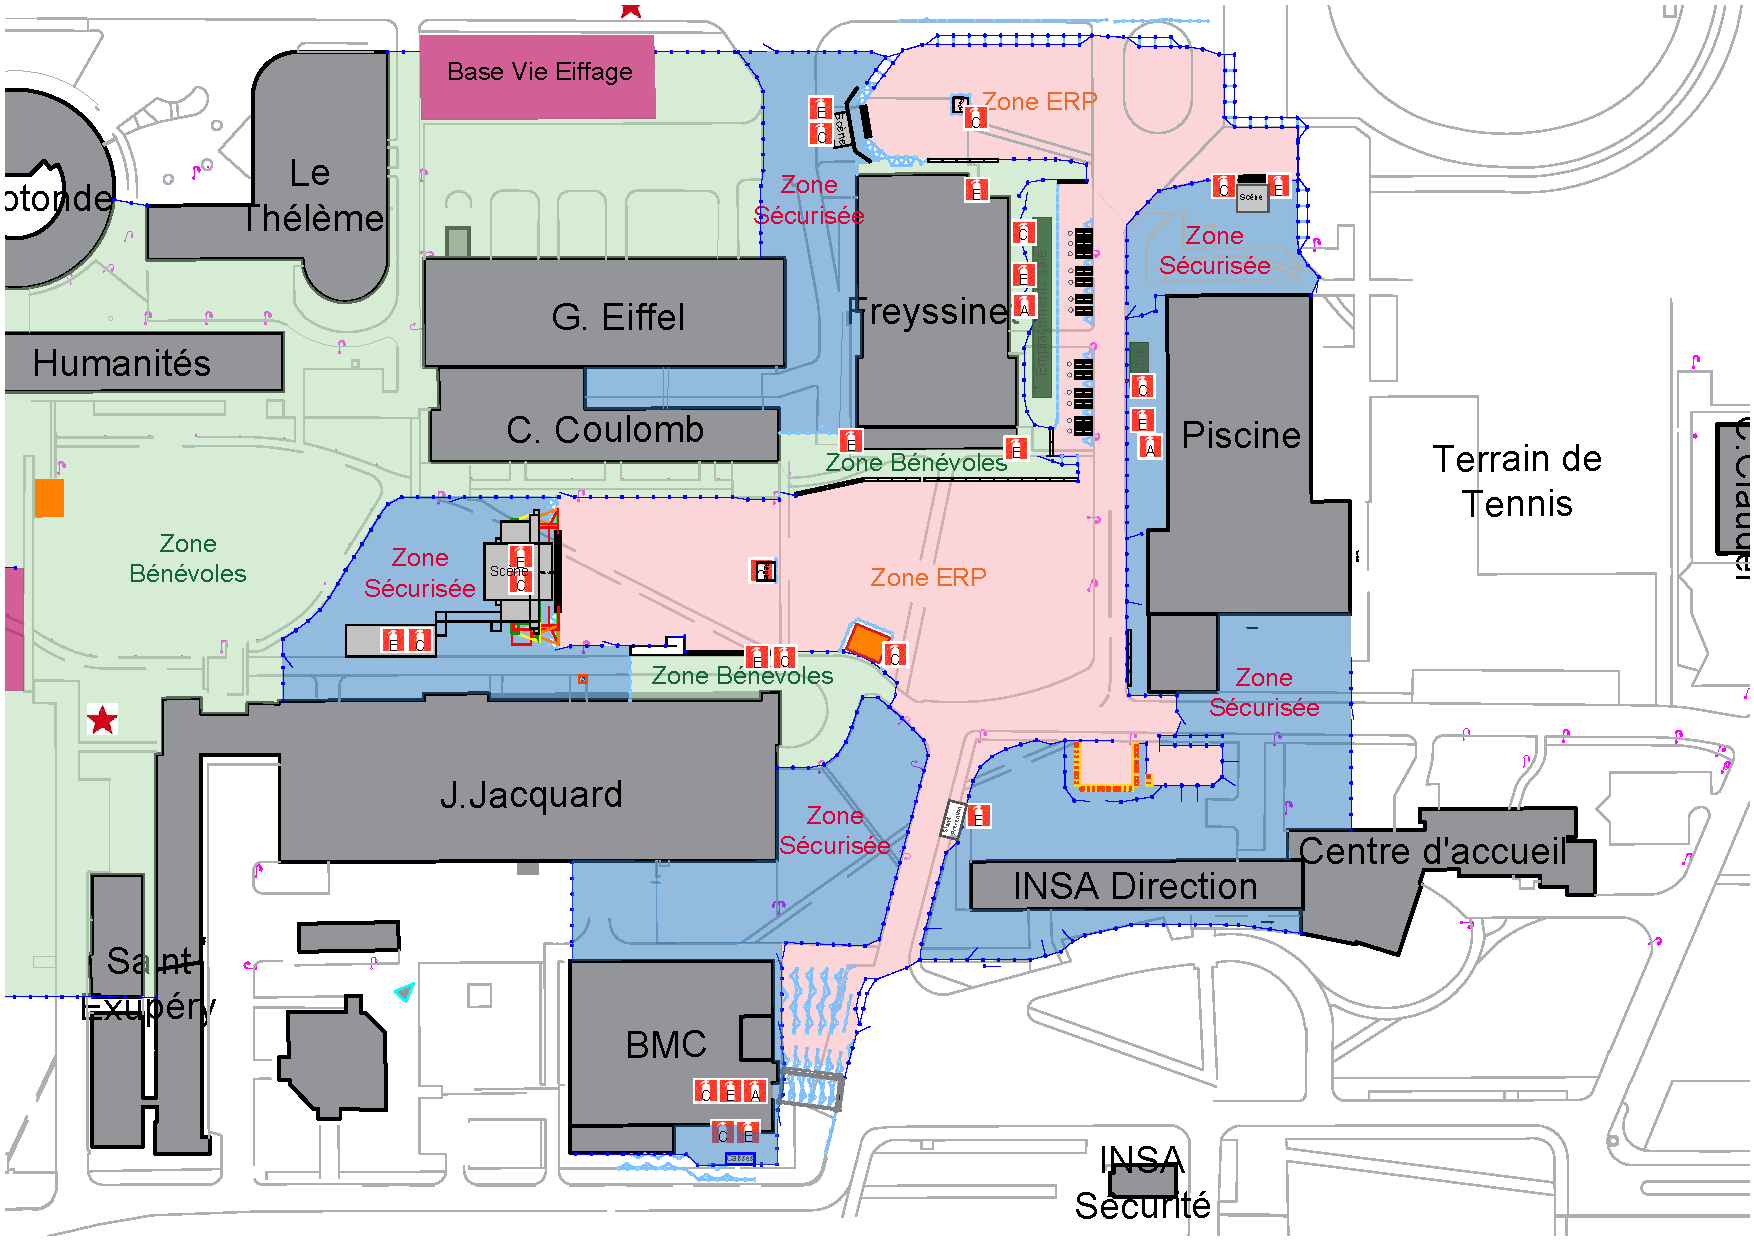
\includegraphics[width=.55\textwidth, trim=150 0 190 0,clip]{Exports/Plan_24h_44eme-Extincteurs}\\
\end{tabular}

\end{frame}

\begin{frame}

\frametitle{Dispositions spécifiques à l'espace restauration}
\begin{tabular}{i{.50\textwidth} c}
\item \textbf{5} concessions salées
\item 1 concessions sucrées
\item Ouverture en \textbf{soirée de 20h à 3h45} et en \textbf{journée de 10h à 18h}
\item Foodtruck et tentes \textbf{ignifugées}
\item Présence d'agents de sûreté pour réguler le flux de personnes
\item Extincteurs A3F, H2O et CO2 à disposition sur place
& 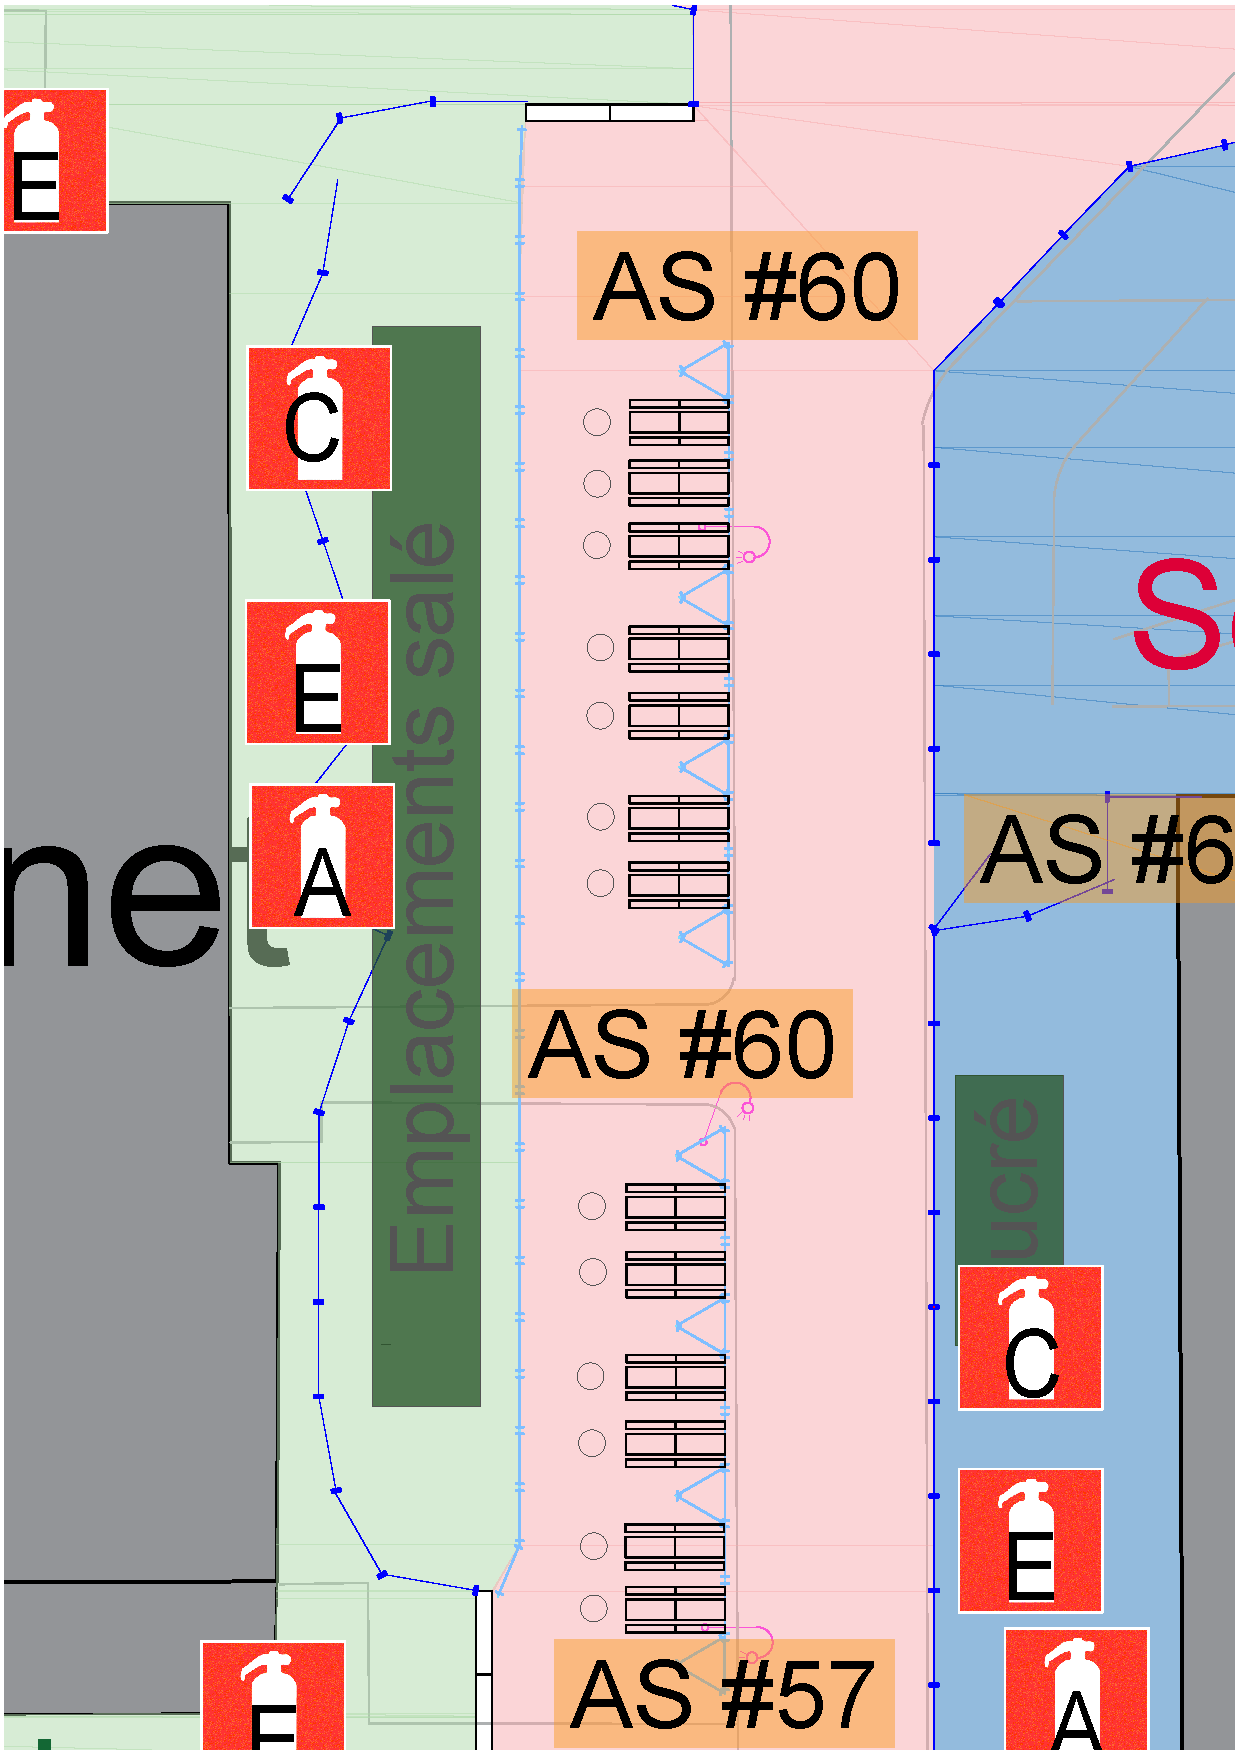
\includegraphics[width=.4\textwidth, trim=0 0 0 0,clip]{Exports/Plan_24h_44eme-Espace_Resto_secu_incendie}\\
\end{tabular}

\end{frame}

\begin{frame}

\frametitle{Troisième scène - Implantation}
\begin{tabular}{i{.35\textwidth} c}
\item \textbf{Principe :} Petite scène, public de 500 personnes environ
\vspace{0.45cm}
\item En soirée : \textbf{20h-3h20}
\vspace{0.45cm}
\item En journée (samedi et dimanche) : \textbf{13h-17h}
\vspace{.5cm}
& 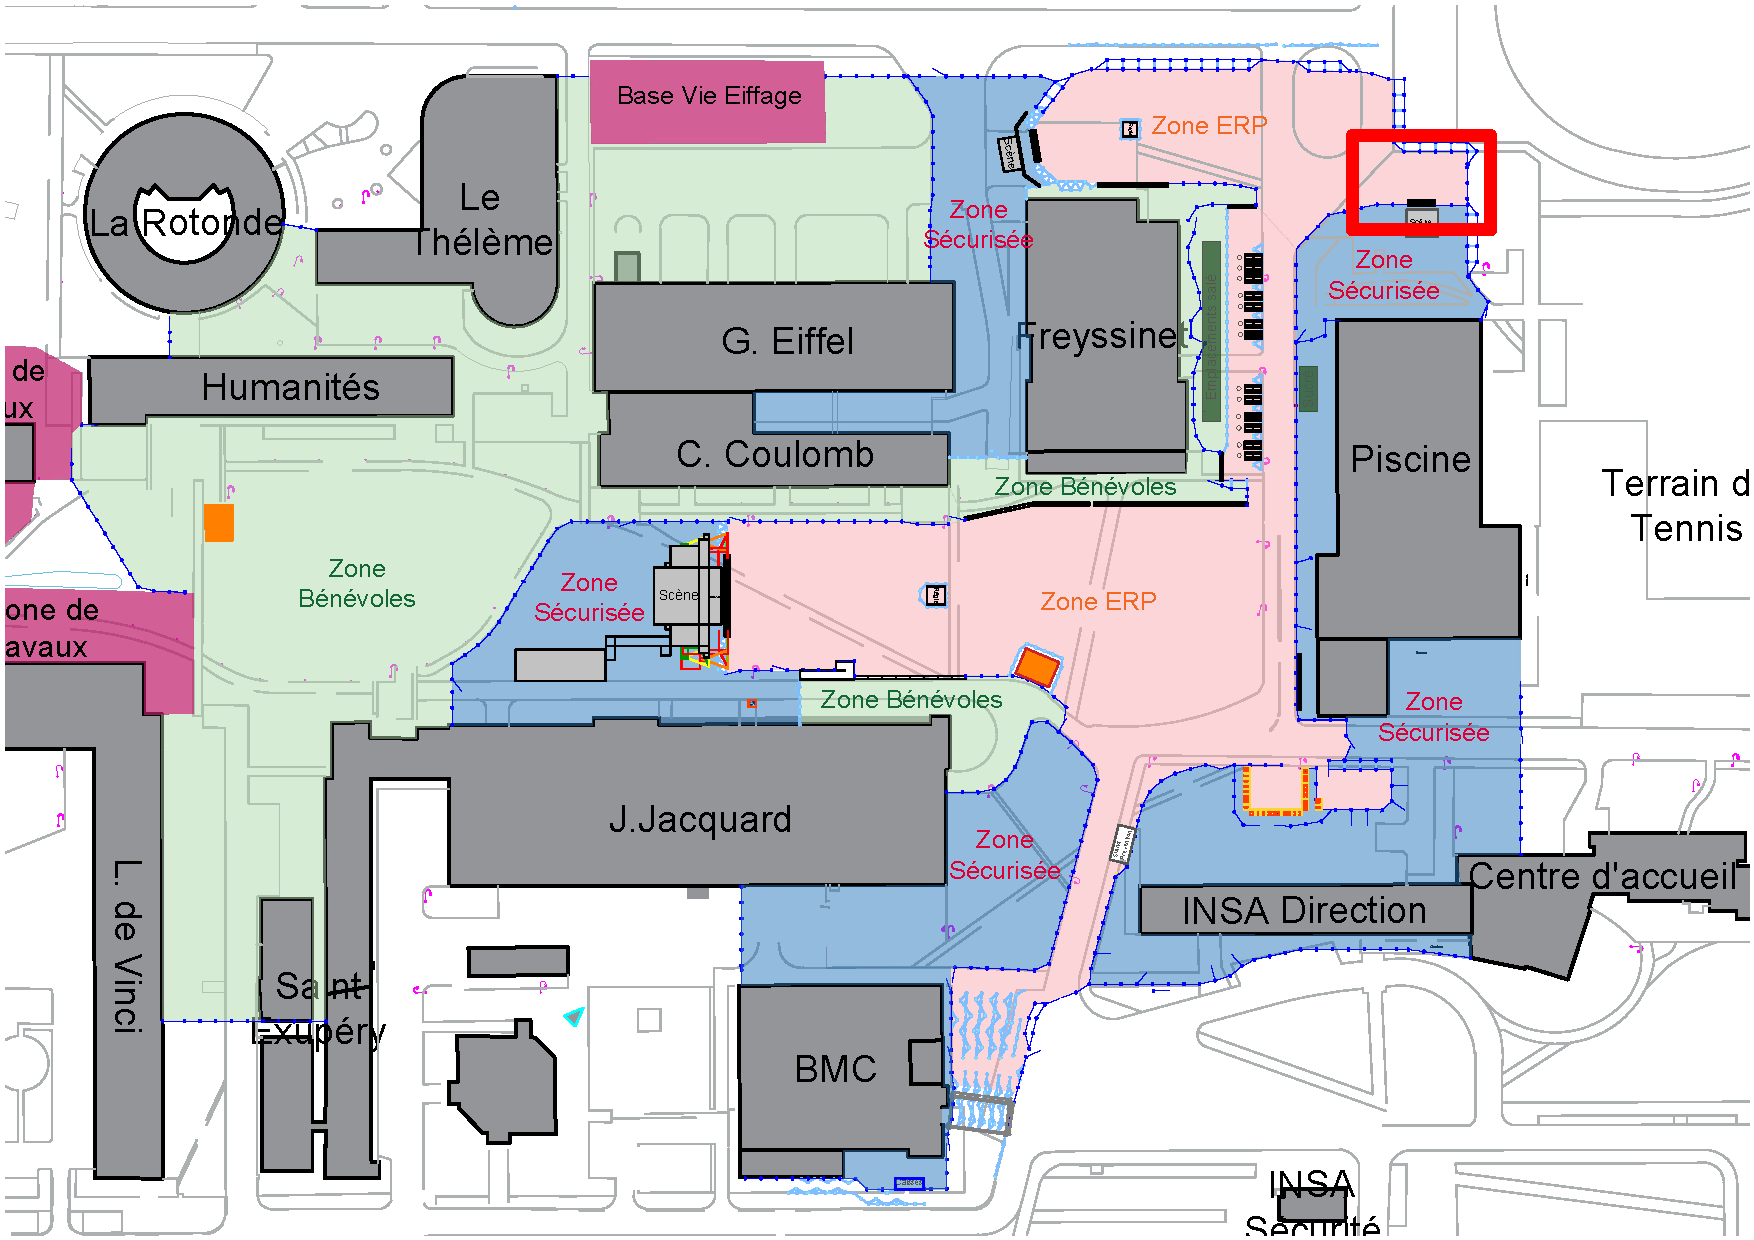
\includegraphics[width=.6\textwidth, trim=300 100 100 0,clip]{Exports/Plan_24h_44eme-3e_Scene}\\
\end{tabular}

\end{frame}

\begin{frame}

\frametitle{Troisième scène - Dispositions de sécurité}
\begin{tabular}{i{.35\textwidth} c}
\item \textbf{2 dégagements} de 4m
\vspace{0.45cm}
\item Mise en place de \textbf{moyens d'extinction} appropriés (CO2 + H2O)
\vspace{0.45cm}
\item Présence de \textbf{3 agents de sûreté} dont 1 \textbf{SSIAP 1}
& 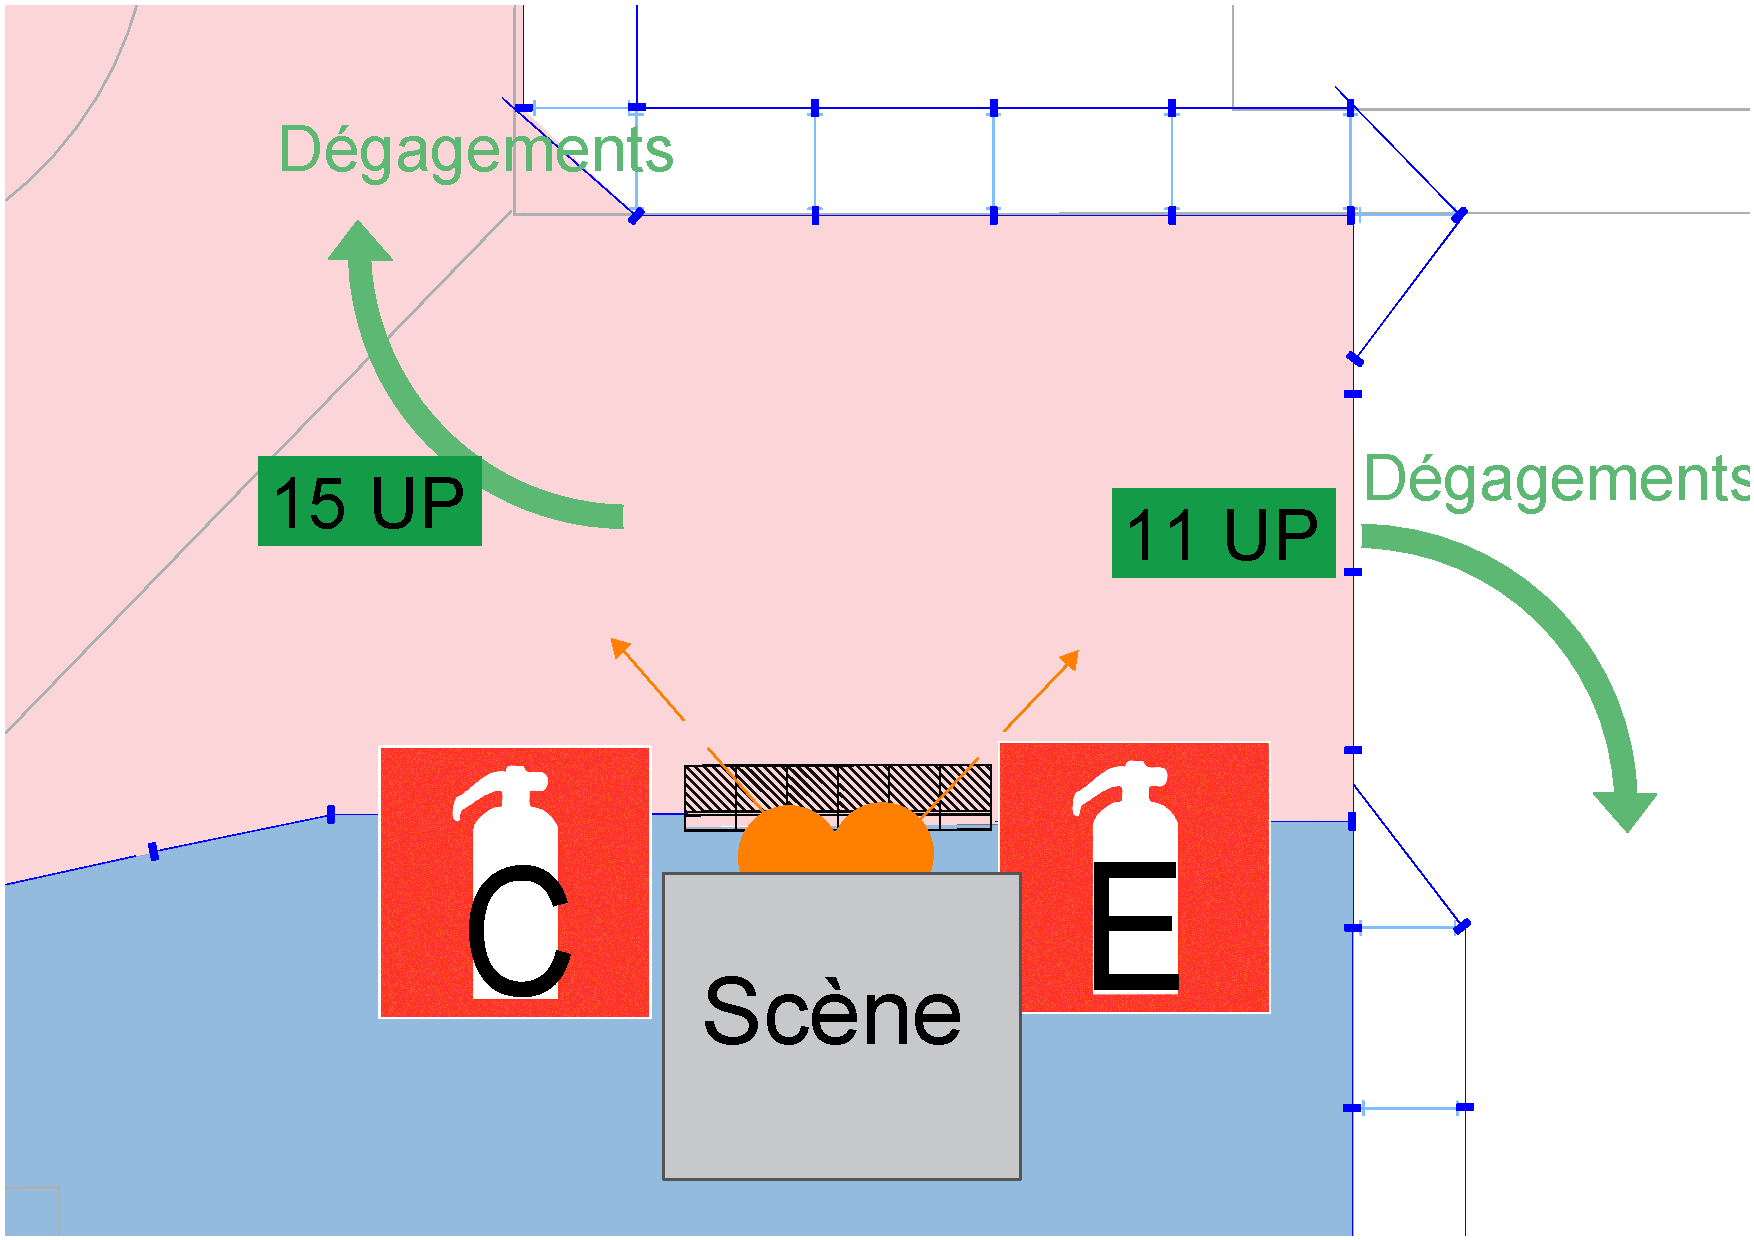
\includegraphics[width=.6\textwidth, trim=0 0 0 0,clip]{Exports/Plan_24h_44eme-3e_Scene_Secu_Incendie}\\
\end{tabular}

\end{frame}

\begin{frame}

\frametitle{Troisième scène - Nouvelles infrastructures scéniques}
\begin{tabular}{i{.35\textwidth} c}
\item Nouvelle structure de scène
\vspace{0.45cm}
\item Mise en place d'une structure décorative surplombant le public
\vspace{0.45cm}
& 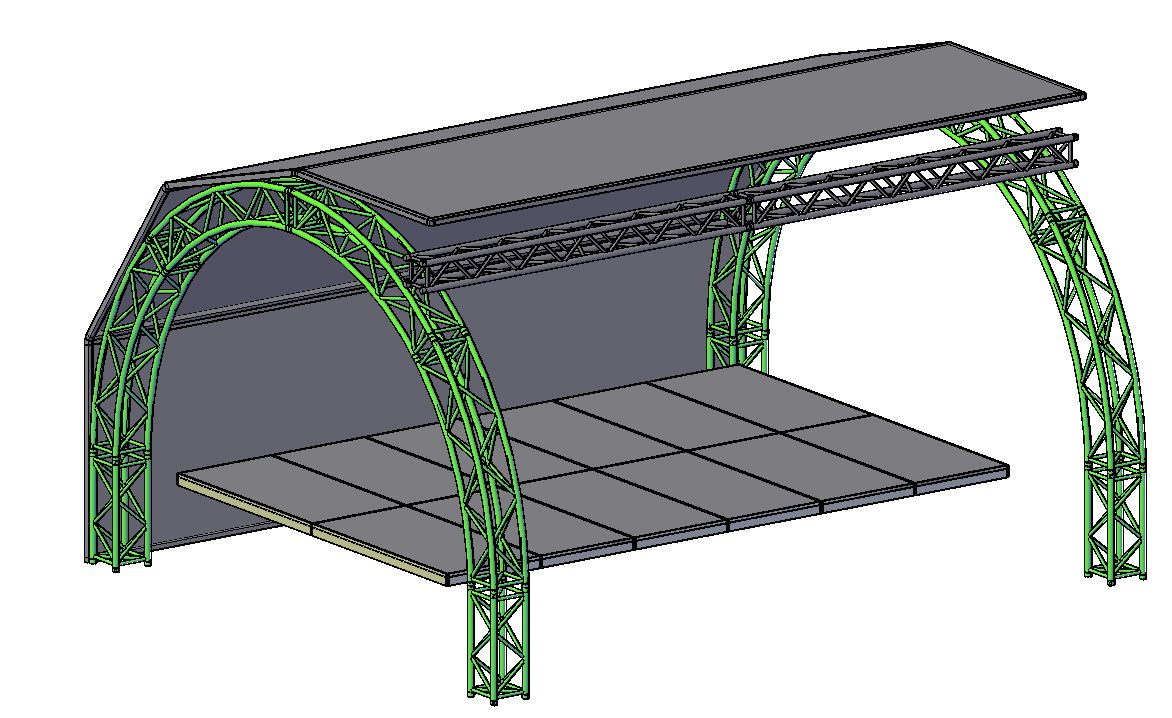
\includegraphics[width=.6\textwidth, trim=0 0 0 0,clip]{Annexes/Images/SceneRoots}\\
\end{tabular}

\end{frame}

\begin{frame}

\frametitle{Troisième scène - Nouvelles infrastructures scéniques}
\centering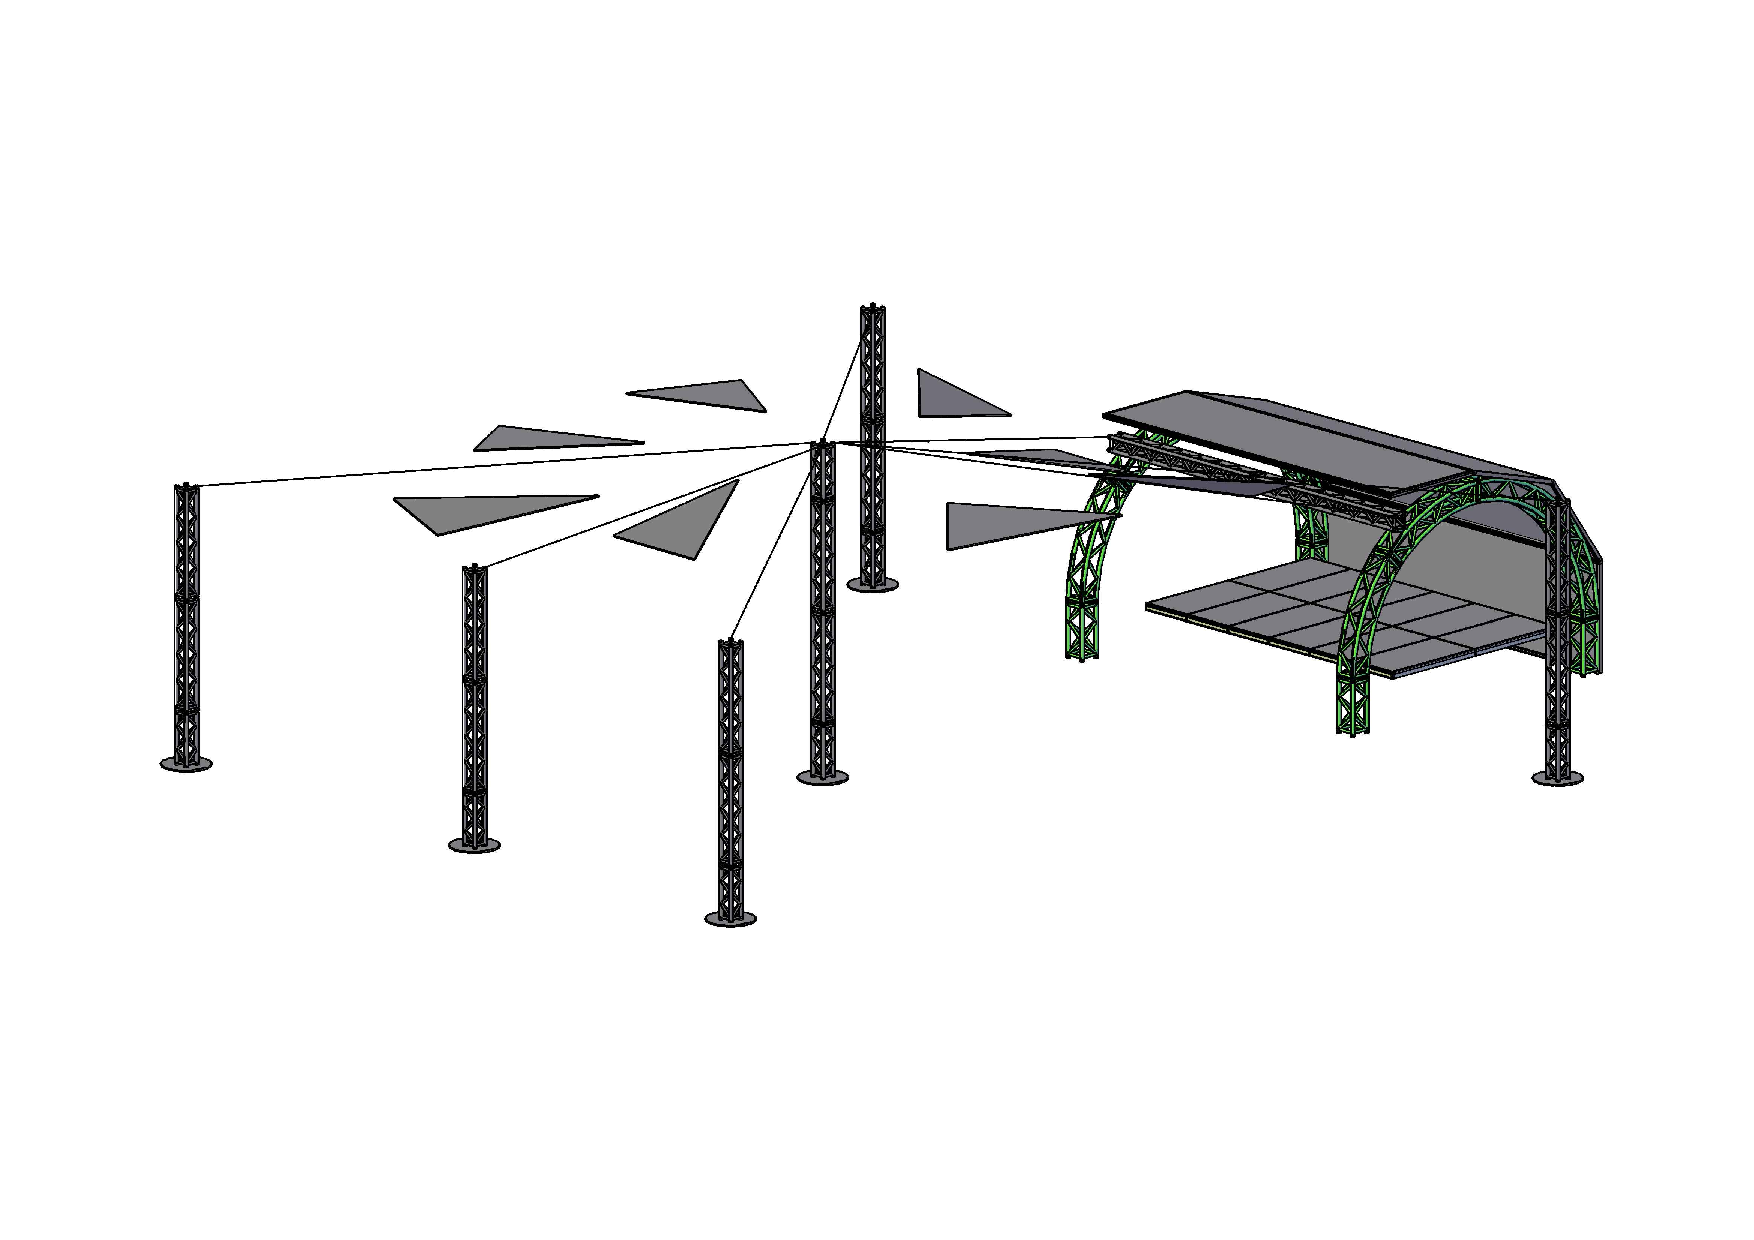
\includegraphics[width=.9\textwidth, trim=0 0 0 0,clip]{Annexes/Images/Totems}

\end{frame}

\begin{frame}

\frametitle{Emplacement PCS \& Croix-Rouge Française}
\begin{tabular}{i{.4\textwidth} c}
\item \textbf{Liaison permanente} avec l'équipe sécurité
\item \textbf{Secouristes} présents pour les soirées de concerts
\item \textbf{Equipes mobiles} patrouillant sur la zone concerts
\item \textbf{Poste de secours} aménagé dans le Gymnase C
\item \textbf {Redirection} des appels du \textbf{CTA}
\item Liaison avec le \textbf{SAMU (15)}
& 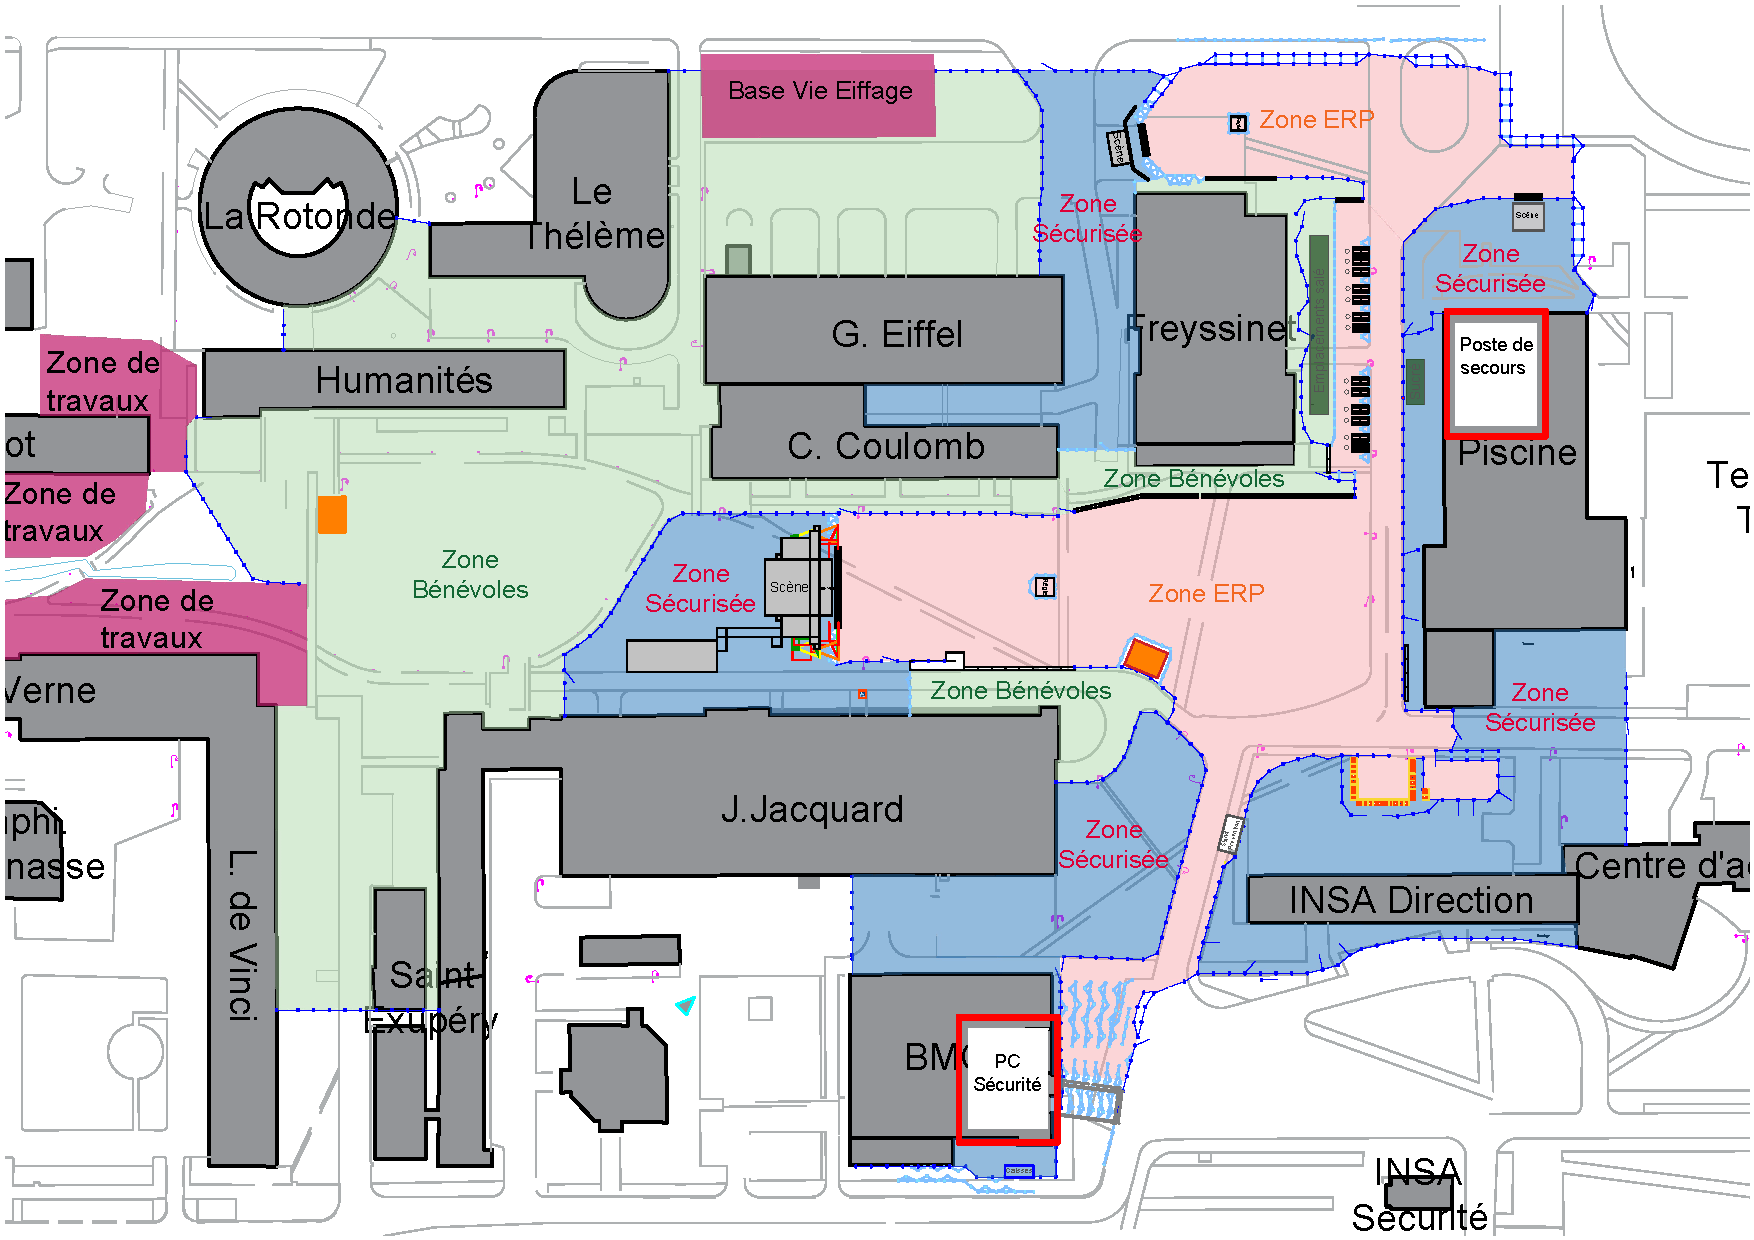
\includegraphics[width=.55\textwidth, trim=350 0 50 0,clip]{Exports/Plan_24h_44eme-PC_Secu}\\
\end{tabular}

\end{frame}

\begin{frame}

\frametitle{Installations électriques}
\begin{itemize}
\item {Eclairage des sorties :}
\begin{itemize}
\item \textbf{Les sorties sont éclairées en permanence}
\item En cas de coupure de courant ou en cas d'évacuation, des \textbf{blocs phares} branchés sur batterie \textbf{éclairents les sorties de secours}
\end{itemize}
\item {Installations électriques :}
\begin{itemize}
\item Présence d'un \textbf{électricien professionnel}
\item Vérifiées par un \textbf{organisme de contrôle}
\item \textbf{Aucune installation n'est à portée du public}
\end{itemize}
\end{itemize}

\end{frame}

\begin{frame}

\frametitle{Zone de caisses}
\begin{tabular}{e{.4\textwidth} c}
\item \textbf{Contrôle visuel} des billets et des sacs par des agents de sûreté
\vspace{.5cm}
\item \textbf{Palpation} par des agents de sûreté
\vspace{.5cm}
\item \textbf{Contrôle} des billets
\vspace{.5cm}
\item \textbf{Accès Zone ERP}
& 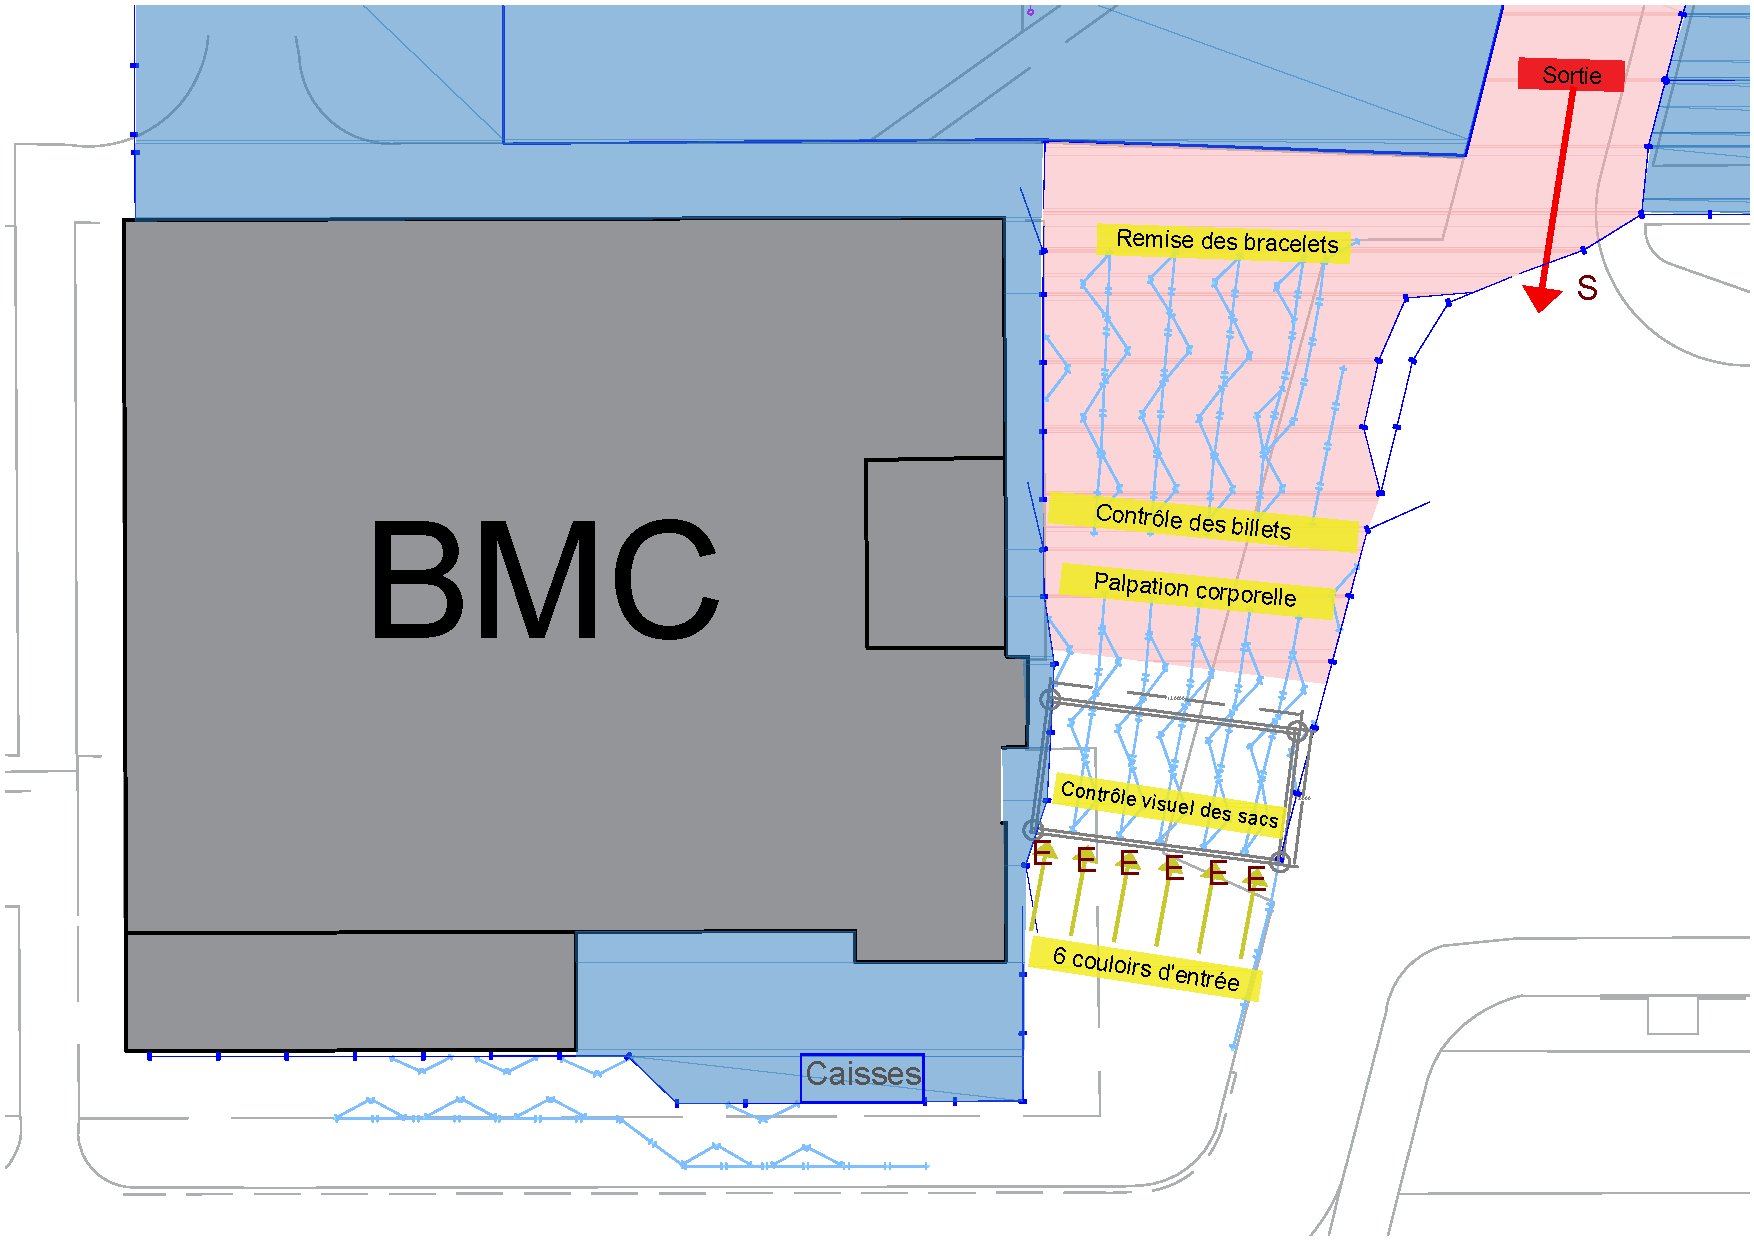
\includegraphics[width=.55\textwidth, trim=0 0 0 0,clip]{Exports/Plan_24h_44eme-Entree_Etapes}\\
\end{tabular}

\end{frame}

\begin{frame}

\frametitle{Grande scène - Nouvelles infrastructures}
\begin{itemize}
\item Etude et montage de la scène par la société Scénétec
\item Vérification par un \textbf{organisme de contrôle}
\end{itemize}
\centering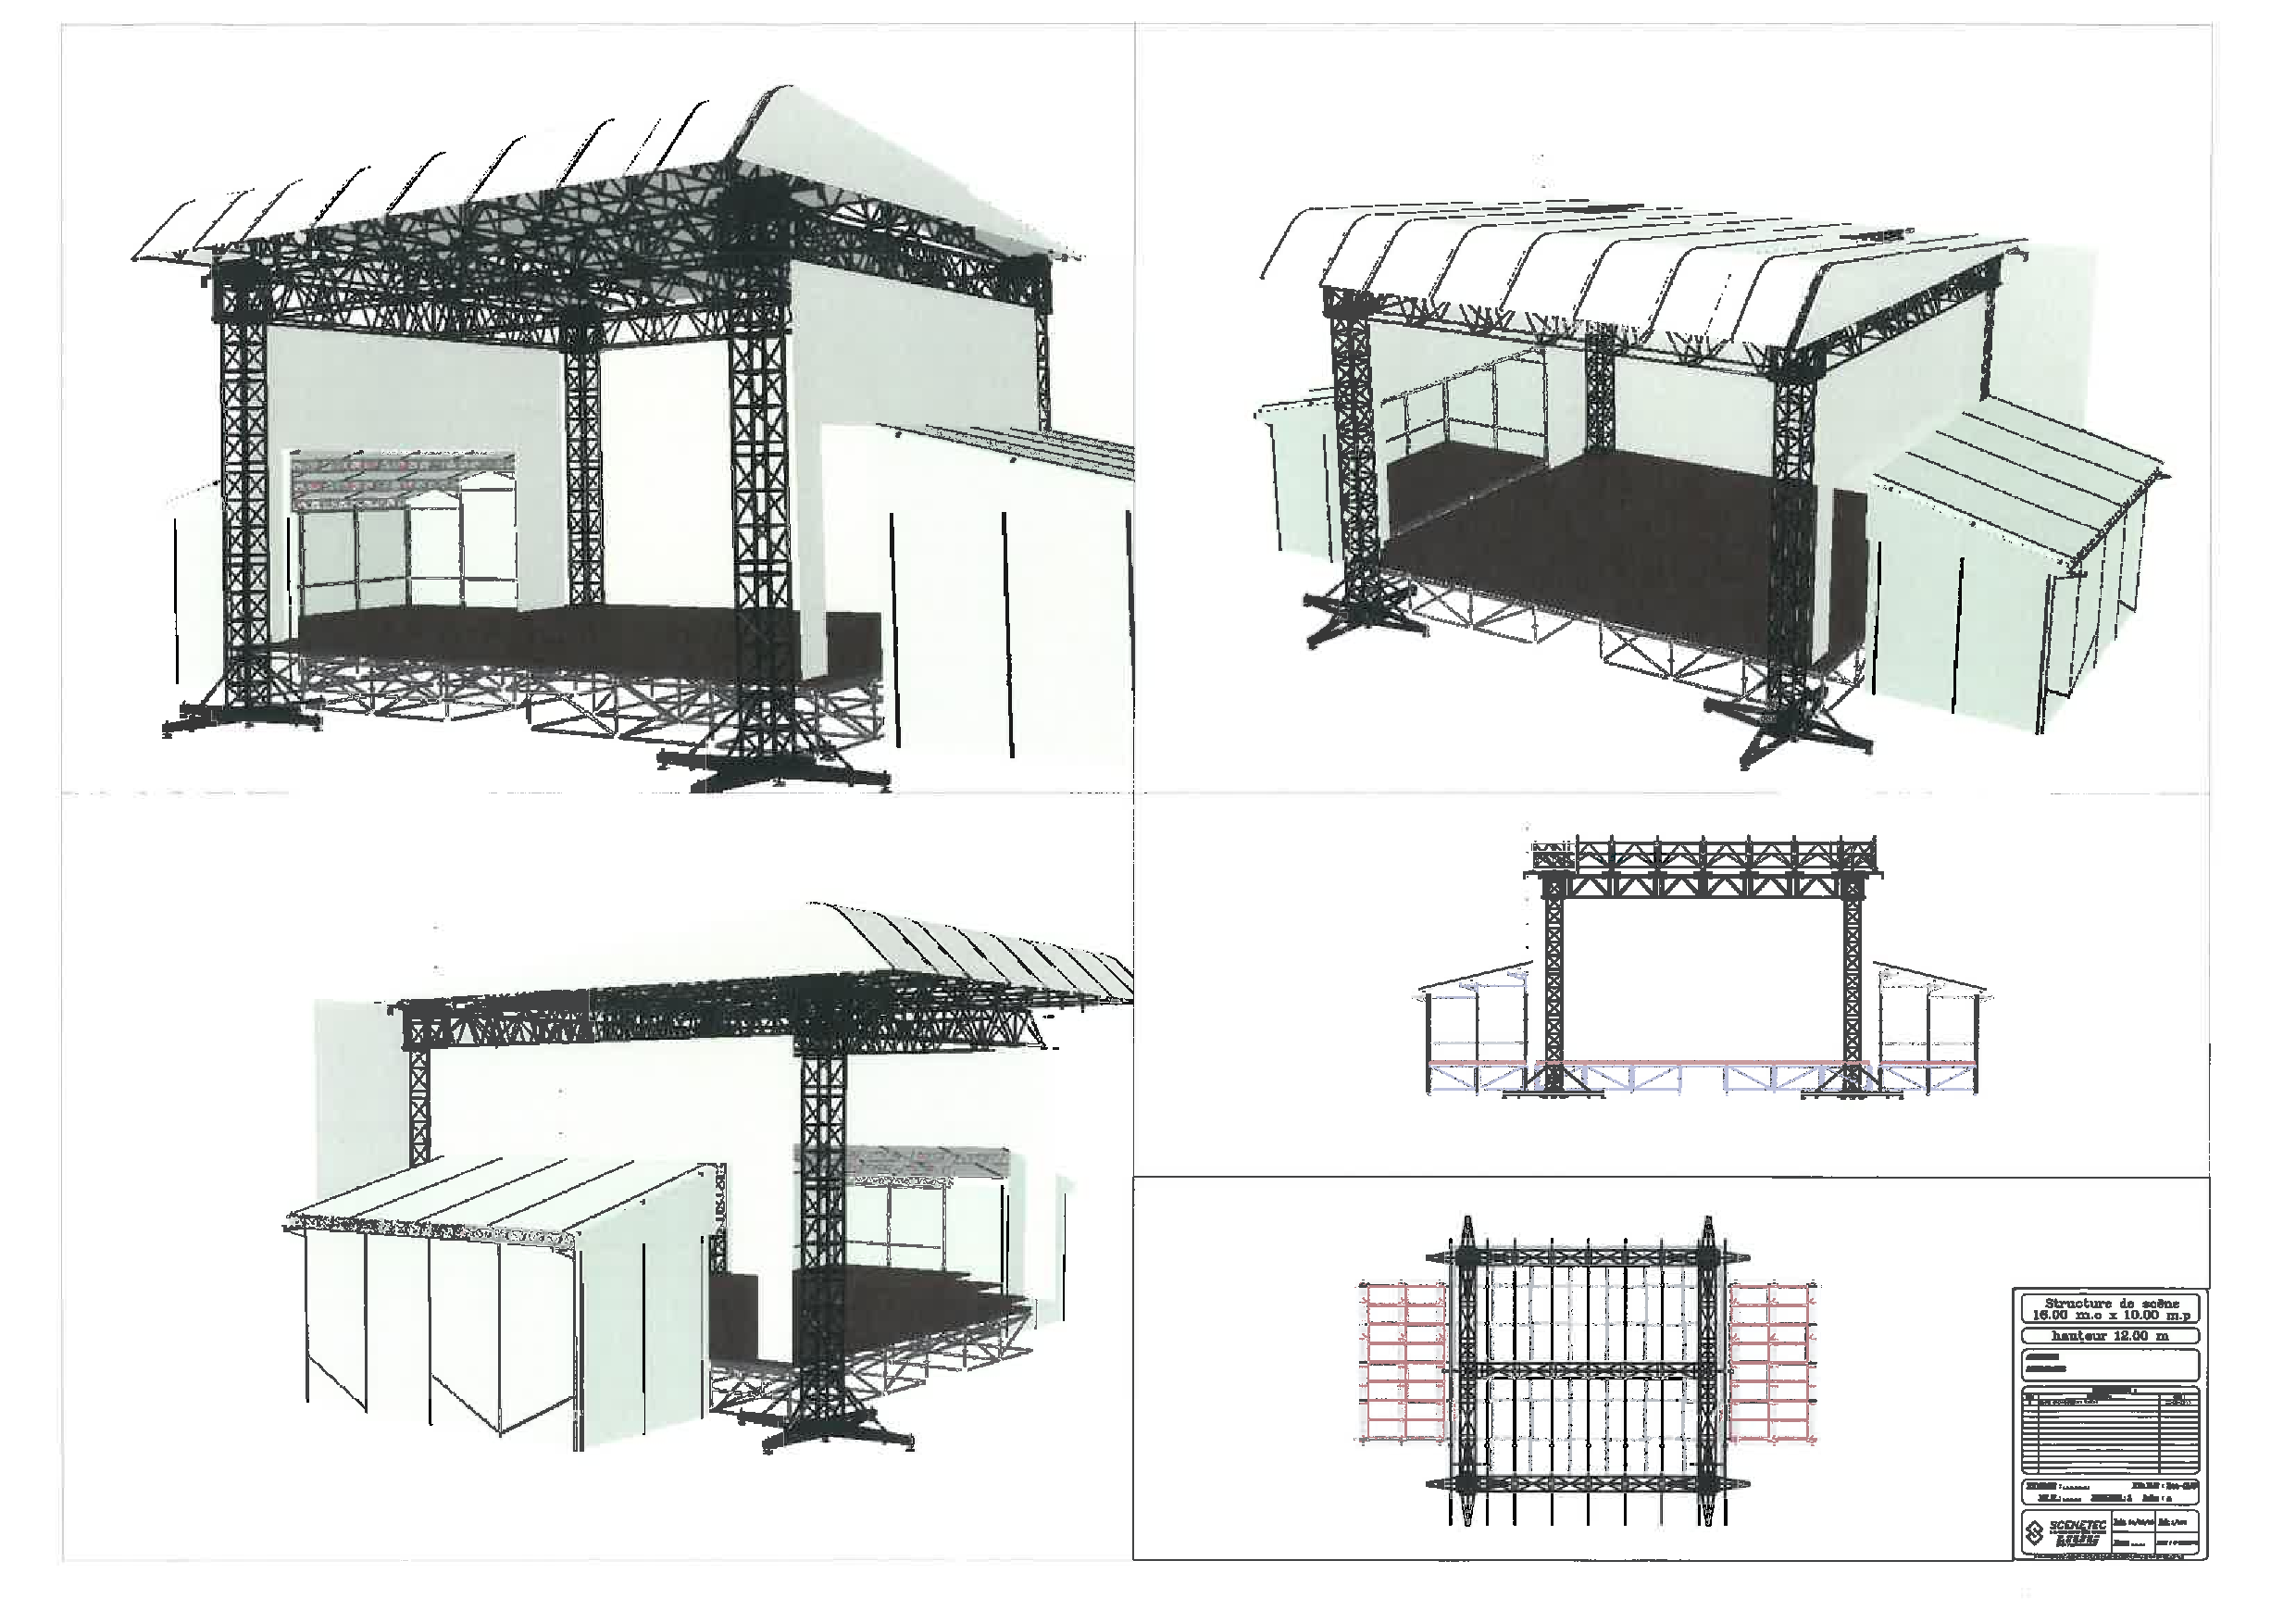
\includegraphics[width=.9\textwidth]{Annexes/Images/GrandeScene}

\end{frame}

\begin{frame}

\frametitle{Risques météorologiques : Pluie}
\textbf{Ne crée pas de risques supplémentaires car :}
\begin{itemize}
\item Installations électriques dans des coffrets \textbf{étanches}
\item Matériel sensible sous \textbf{tentes}
\end{itemize}
\end{frame}

\begin{frame}

\frametitle{Risques météorologiques : Vent}
\begin{itemize}
\item \textbf{Surveillance} : anémomètre, veille météo
\item Vent \textbf{faible} :
\begin{itemize}
\item Tout est \textbf{accroché} (signalétique, banderoles…)
\item Bars \textbf{lestés} (500kg par bar) 
\item Clôtures fixées (jambe de force ou poteau)
\item Bâches micro-perforées
\end{itemize}
\item Vent fort :
\begin{itemize}
\item Scène validée jusqu’à 110 km/h en vent établi
\item Descente du toit au-delà 
$\rightarrow$ Annulation des concerts et évacuation de la zone
\end{itemize}
\end{itemize}

\end{frame}

%========================================
%PROCEDURES D'URGENCE
%========================================

\section{Procédures d'urgence}

\begin{frame}

\centering\Huge{\textbf{Procédures d'urgence}}

\end{frame}

\begin{frame}

\frametitle{Plan d'action en cas d'urgence}
\begin{center}
\begin{tikzpicture}[thick]
  \node[draw,rectangle,minimum height=3cm,minimum width=4cm, text width=4cm,rounded corners=0.5cm,fill=green!40] at (0,4)(a) {%
  \begin{tabular}{>{\centering\arraybackslash} m{3.5cm}}
  \textbf{Fonctionnement normal}\\
  
  \end{tabular}
  };
  \node[draw,rectangle,minimum height=3cm,minimum width=4cm, text width=4cm,rounded corners=0.5cm,fill=ALUFblue!30] at (5,4) (b) {%
  \begin{tabular}{>{\centering\arraybackslash} m{3.5cm}}
  \textbf{Situation renforcée}\\ \vspace{2mm}
  \begin{itemize}
  \scriptsize
  \item Mise en place d'une vigie
  \item Possibilité d'arrêt des concerts
  \end{itemize}\\
  \end{tabular}};
  \node[draw,rectangle,minimum height=3cm,minimum width=4cm, text width=4cm,rounded corners=0.5cm,fill=ALUFblue!80] at (5,0) (c) {%
  \begin{tabular}{>{\centering\arraybackslash} m{3.5cm}}
  \textbf{Situation d'évacuation}\\
  \begin{itemize}
  \scriptsize
  \item Evacuation de la Zone Concerts et/ou ouverture des issues de secours
  \item Alerte donnée aux services publics et de secours
  \end{itemize}
  \end{tabular}};
  \node[draw,rectangle,minimum height=3cm,minimum width=4cm, text width=4cm,rounded corners=0.5cm,fill=ALUFred!60] at (0,0) (d) {%
  \begin{tabular}{>{\centering\arraybackslash} m{3.5cm}}
  \textbf{Situation de crise}\\
  \begin{itemize}
  \scriptsize
  \item Ouverture des PMA
  \item Armement du PCO
  \end{itemize}\\
  \end{tabular}};

  % 1st pass: draw arrows
  \draw[vecArrow] (a) to (b);
  \draw[vecArrow] (b) to (c);
  \draw[vecArrow] (c) to (d);

\end{tikzpicture}
\end{center}

\end{frame}

\begin{frame}

\frametitle{Plan d'accès des secours}
\begin{tabular}{i{.35\textwidth} c}
\item \textbf{Adresse unique :} 20 avenue Albert Einstein
\item \textbf{Point de ralliement :} poste de garde de l'INSA
\item \textbf{PMA possibles :} Gymnases, terrain de sport, hall Marie Curie
& 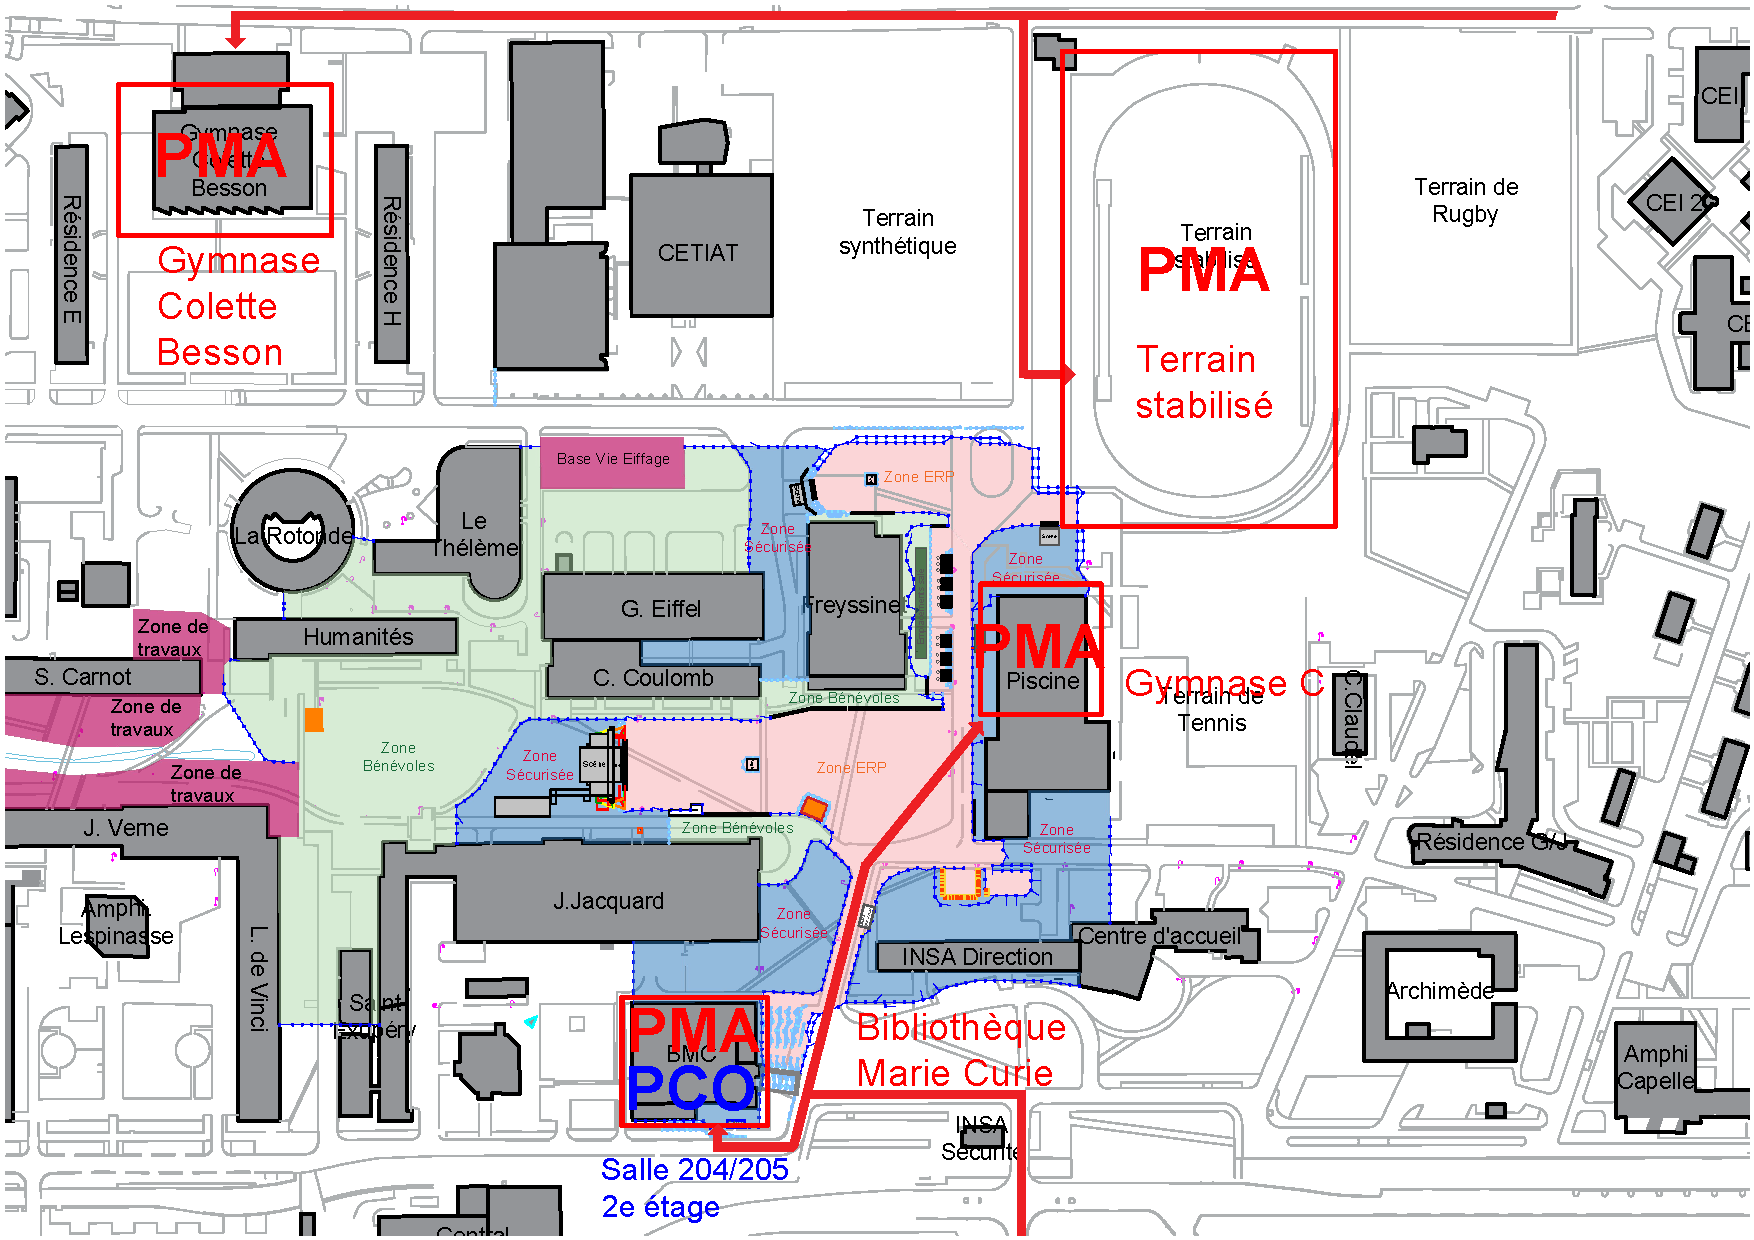
\includegraphics[width=.6\textwidth, trim=0 0 150 0,clip]{Exports/Plan_24h_44eme-PCO_PMA}\\
\end{tabular}

\end{frame}

\begin{frame}

\frametitle{Evacuation des PMR}
\begin{itemize}
\item Présence d’un agent \textbf{SSIAP 1} à proximité de la rampe PMR et présence d’une dizaine de bénévoles à la buvette à proximité.
\vspace{.5cm}
\item Message d’évacuation \textbf{sonore et visuel} pour les malentendants et malvoyants
\vspace{.5cm}
\item Agents de sûreté aux issues de secours
\end{itemize}

\end{frame}

%========================================
%DISPOSITIF DE SURETE
%========================================

\section{Dispositif de sûreté}

\begin{frame}

\centering\Huge{\textbf{Dispositif de sûreté}}

\end{frame}

\begin{frame}

\frametitle{L'équipe sécurité des 24 heures de l'INSA}
\begin{itemize}
\item Mise en place d'un \textbf{PC sécurité}
\vspace{.3cm}
\item \textbf{Permanence 24h/24}
\vspace{.3cm}
\item Tenue de la \textbf{main courante}
\vspace{.3cm}
\item \textbf{Coordination} des différents acteurs :
\begin{itemize}
\item Présence des responsables de \textbf{STAFF Sécurité} et \textbf{Croix-Rouge} 
\item \textbf{Liaison radio} avec les organisateurs
\item Liaison avec les \textbf{services de secours}
\item Liaison avec le service de prevention \& de sécurité de l’INSA
\item Liaison avec le PC sécurité TCL
\end{itemize}
\vspace{.3cm}
\item Ligne principale : 04 28 29 63 82
\item Ligne secondaire : 04 72 43 70 70
\end{itemize}

\end{frame}

\begin{frame}

\frametitle{Les agents de sûreté (AS)}
\begin{tabular}{i{.4\textwidth} c}
\item \textbf{Société STAFF Sécurité}
\item \textbf{Agents de sécurité} incendie : 1 SSIAP 3, 2 SSIAP 2, 5 SSIAP 1
\item Jusqu'à \textbf{85 AS} aux heures de pointe
\item \textbf{Liaison radio permanente} avec l'équipe sécurité
\item \textbf{6 équipes cynophiles} (1 maître-chien + 1 AS + 1 chien)
& 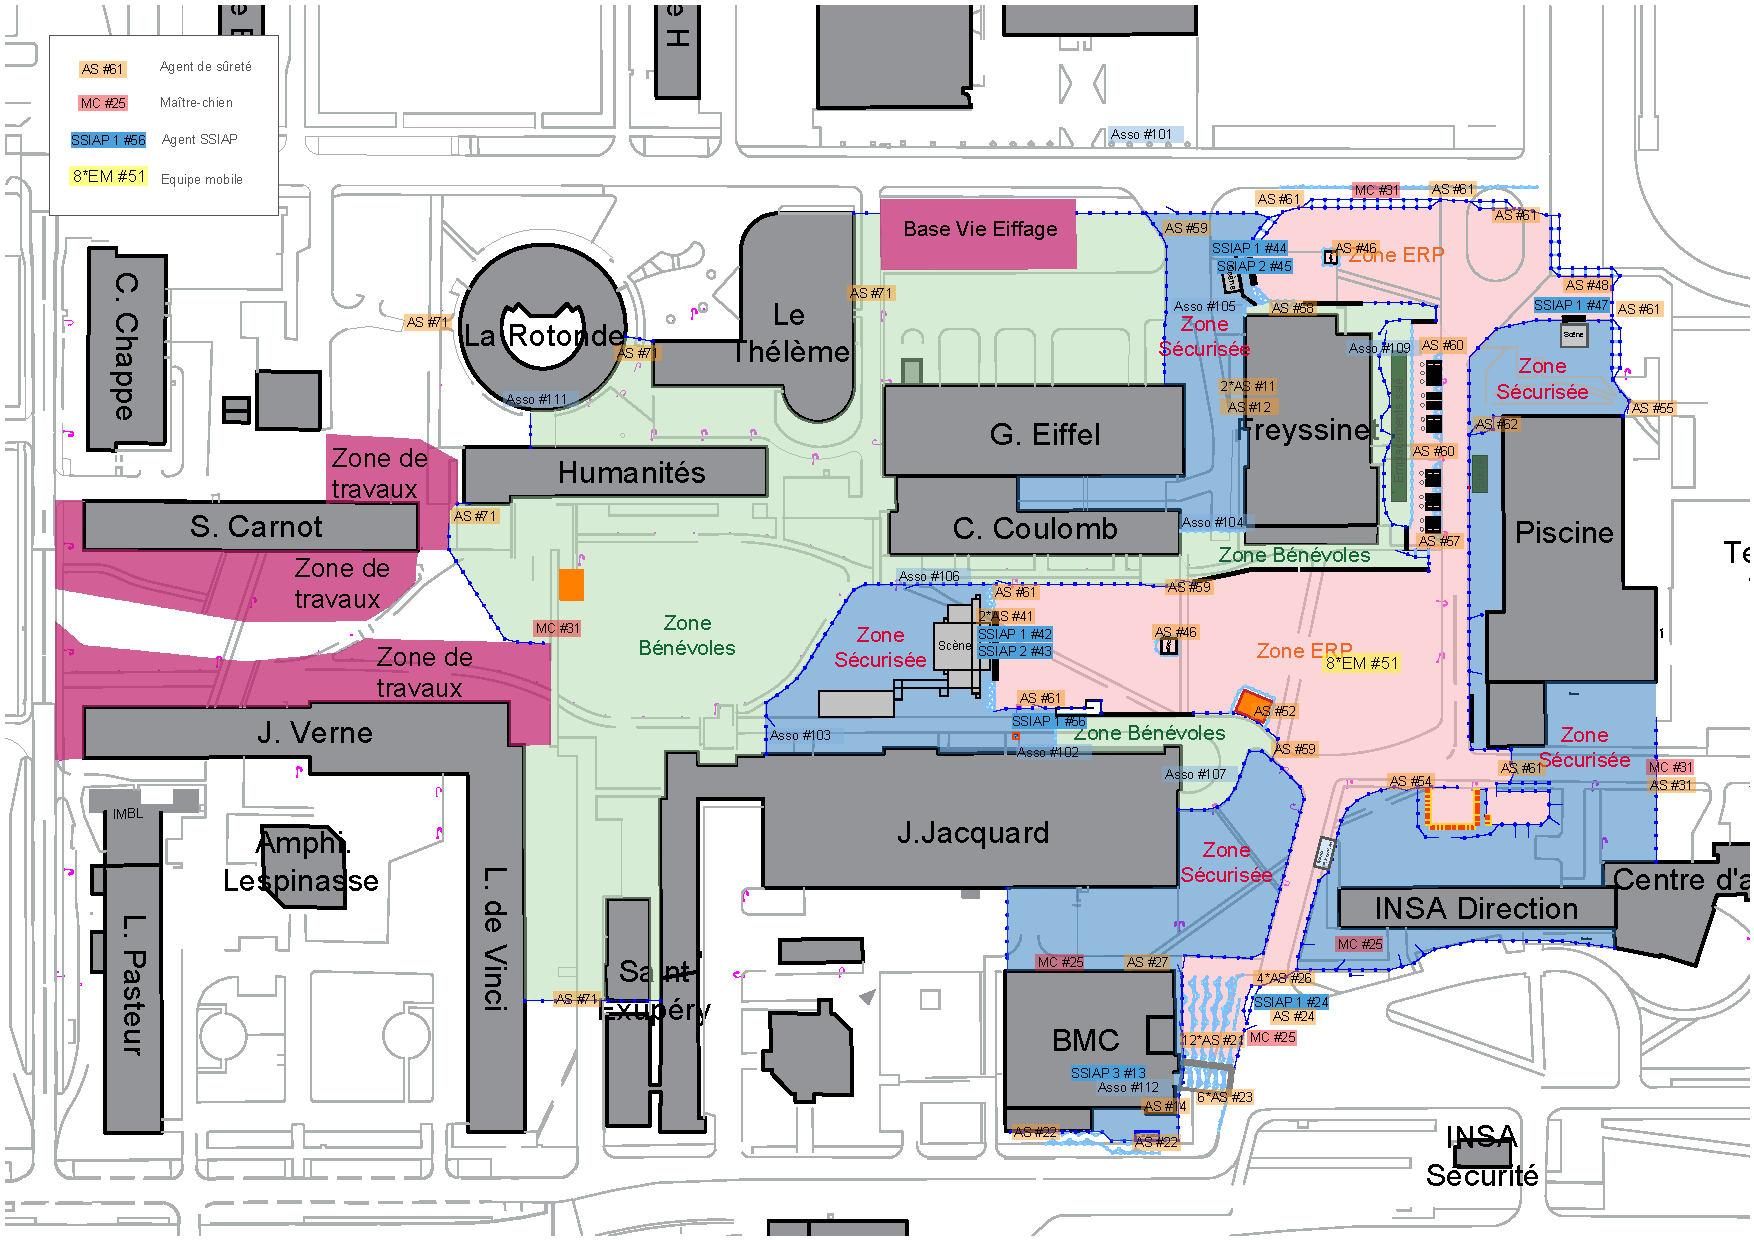
\includegraphics[width=.55\textwidth, trim=350 0 30 50,clip]{Exports/Plan_24h_44eme-AS_Nuit}\\
\end{tabular}


\end{frame}

\begin{frame}

\frametitle{Les agents de sûreté (AS) - Zone des caisses}
\begin{tabular}{i{.45\textwidth} c}
\item \textbf{Equipe mobile} : 1 SSIAP 1 + 1 agent + 1 maître-chien
\item \textbf{Palpation} 12 agents
\item \textbf{Files} 6 agents
\item \textbf{Sortie} 4 agents
\item \textbf{Caisses} 3 agents
\item \textbf{Alentours} : 2 maîtres-chiens + 1 AS
\item \textbf{Total} : 31 agents sur la zone
\item \textbf{Evacuation de l'argent :} Couloir de circulation en zone sécurisée
& 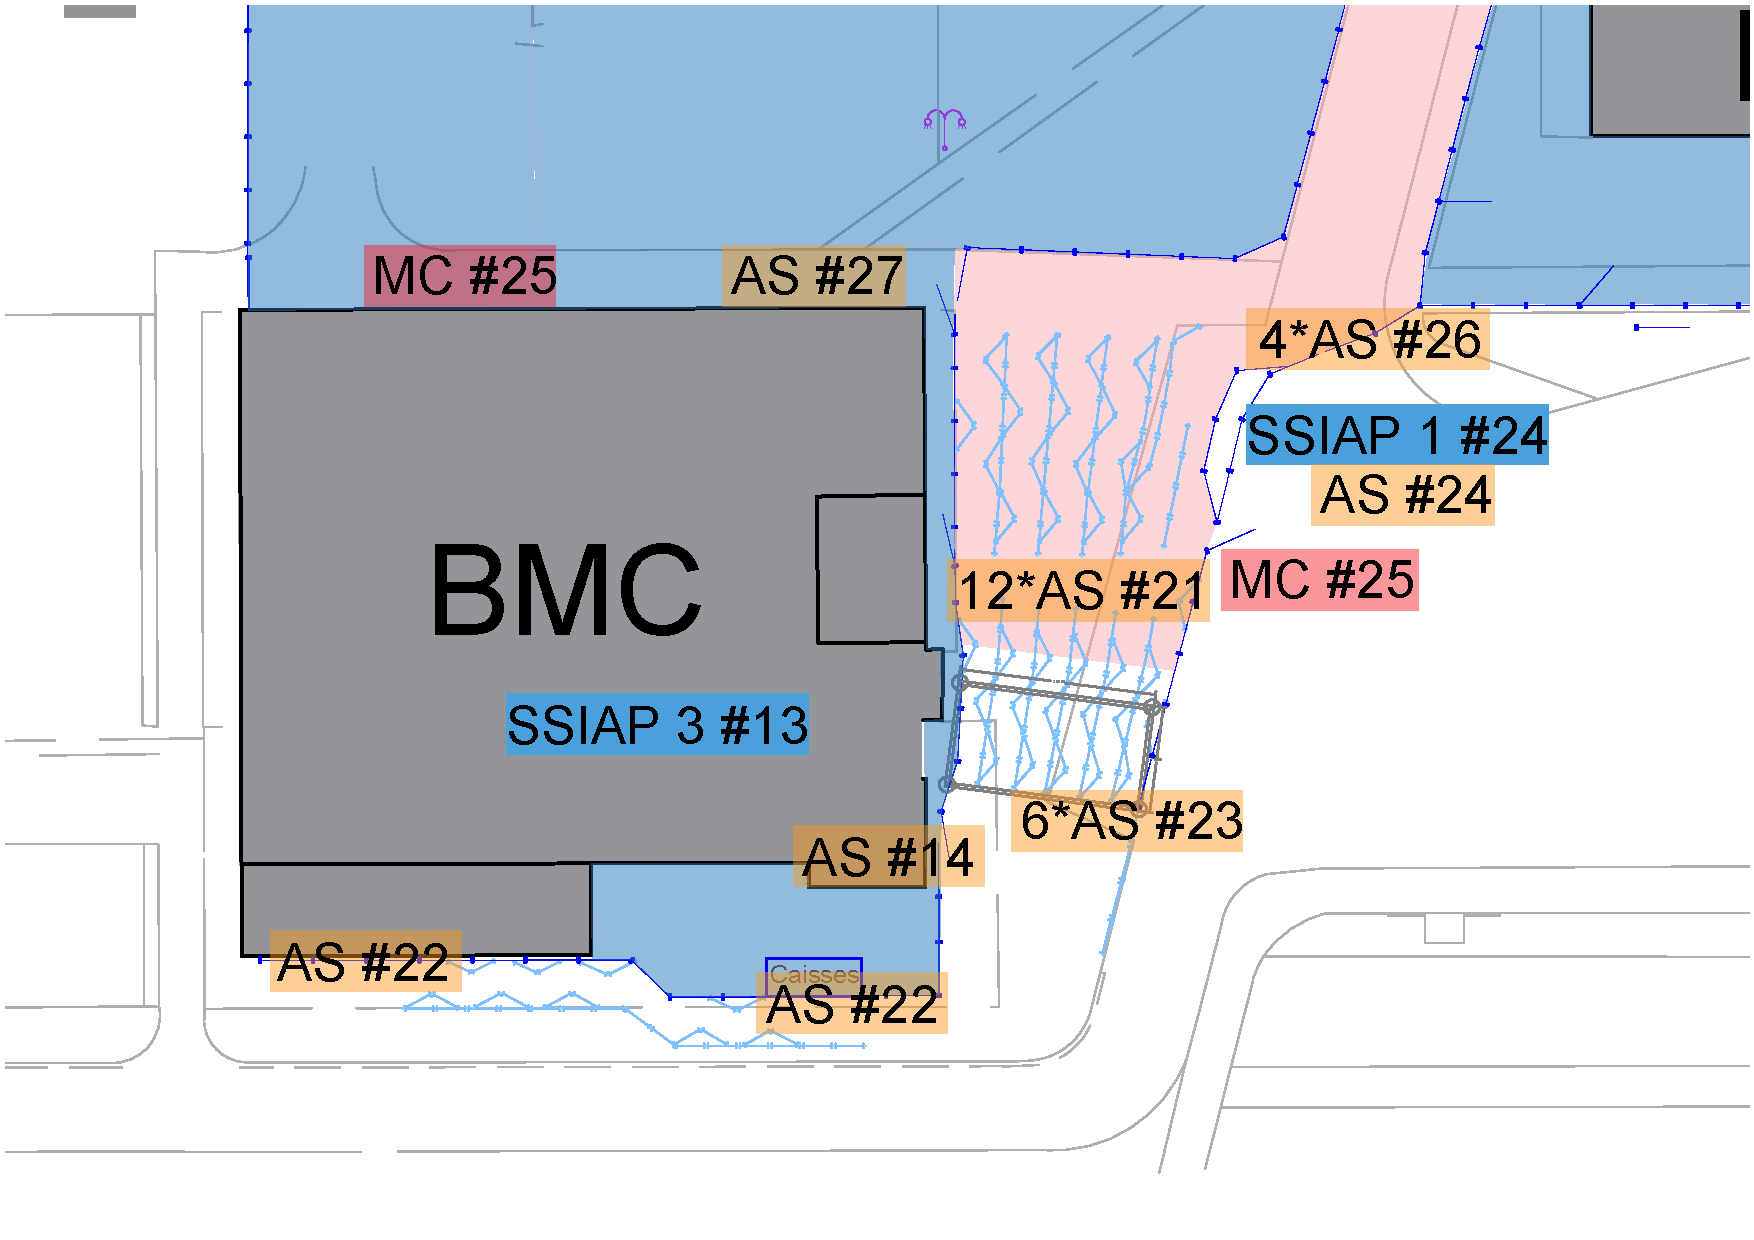
\includegraphics[width=.5\textwidth, trim=100 0 50 0,clip]{Exports/Plan_24h_44eme-Entree_AS}\\
\end{tabular}

\end{frame}

\begin{frame}

\frametitle{Dispositions spécifiques liées à la "Travée Verte"}
\begin{tabular}{i{.4\textwidth} c}
\item Dispositif en place depuis 4 ans avec d'excellents résultats
\vspace{.3cm}
\item Mis en place les \textbf{vendredi et samedi de 20h à 9h}
\vspace{.3cm}
\item Présence d'agents pour ouvrir les \textbf{voies pompiers}
& 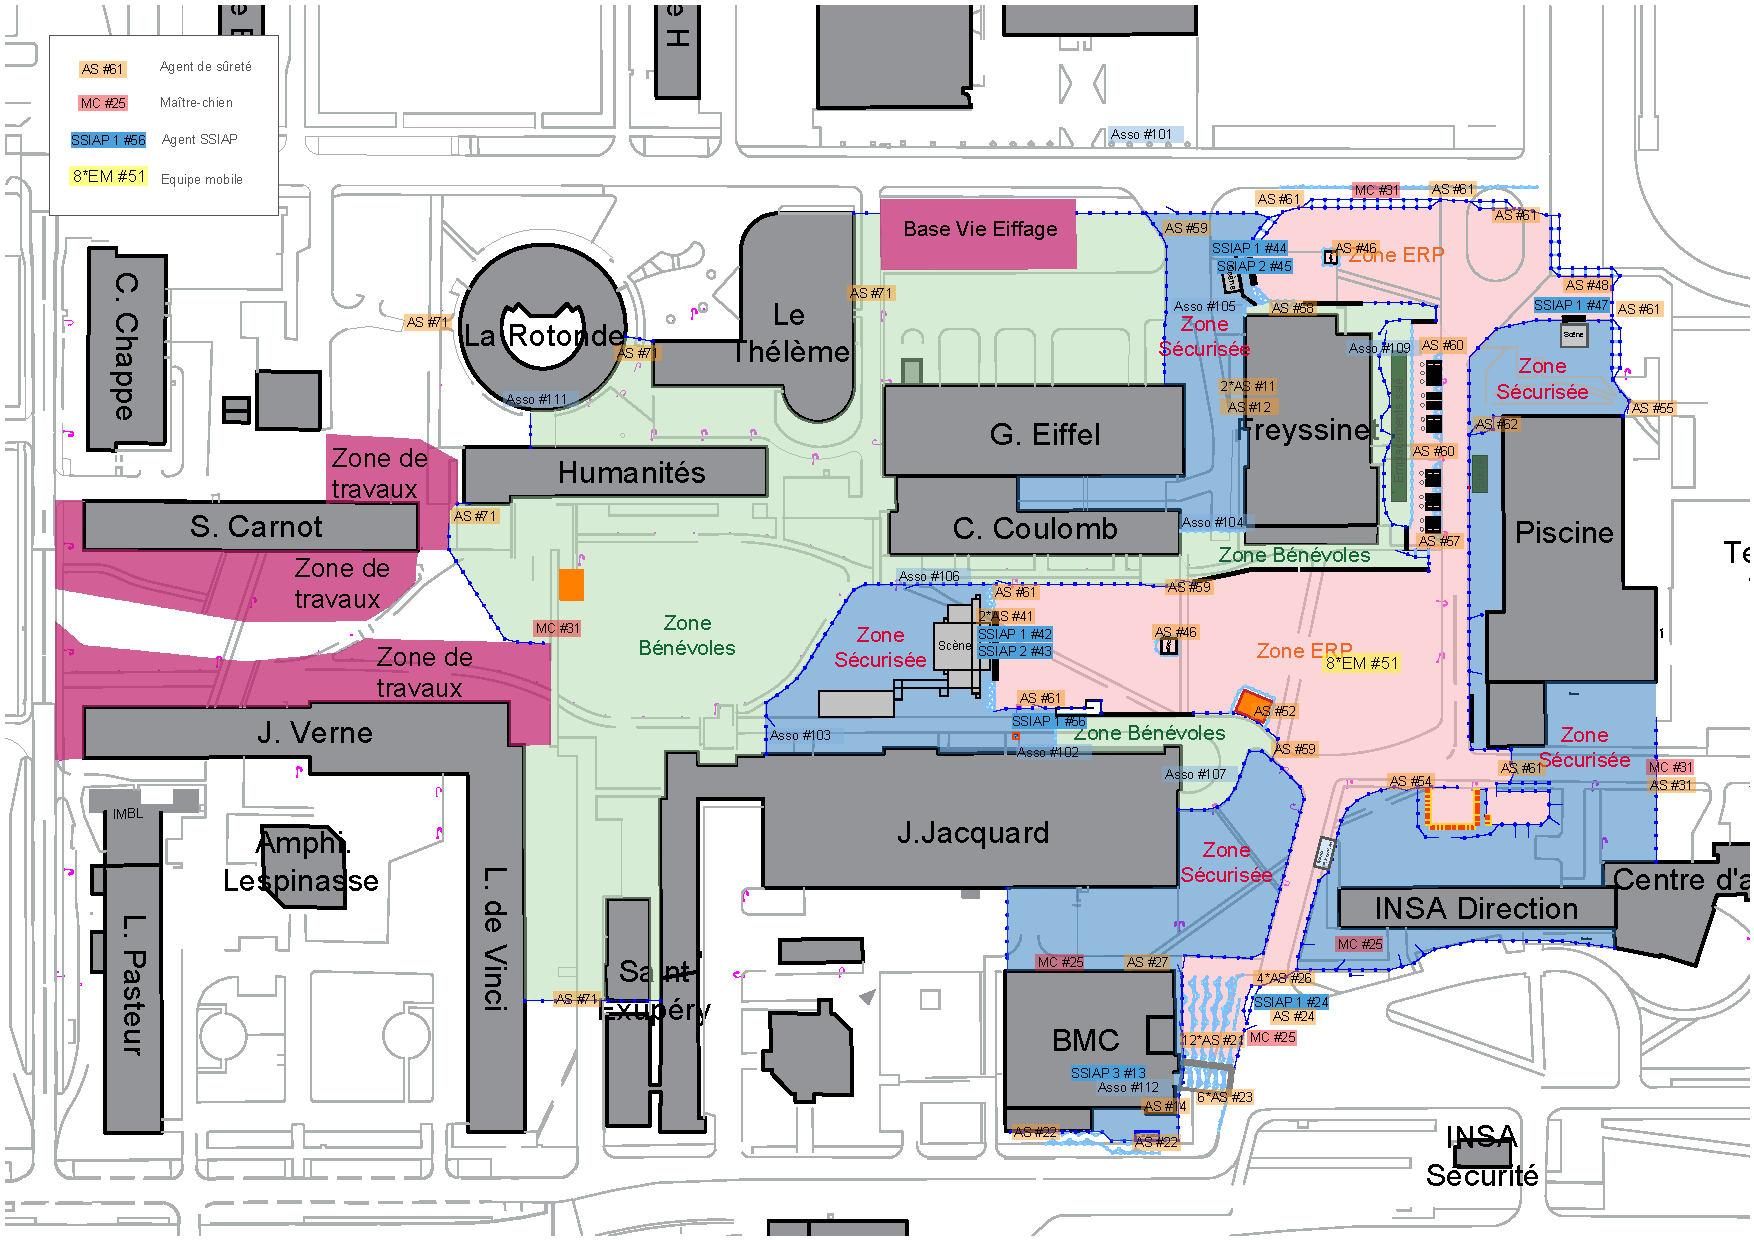
\includegraphics[width=.55\textwidth, trim=0 80 350 100,clip]{Exports/Plan_24h_44eme-AS_Nuit}\\
\end{tabular}

\end{frame}

\begin{frame}

\frametitle{Prise en compte du plan Vigipirate}
\begin{itemize}
	\item Gérer la sûreté et la sécurité des événements et sites culturels - Edition avril 2017
	\item Note de posture Vigipirate du 2 novembre 2017
	\item Fiches mesures :
	\begin{list}{-}{}
		\item Recommandations pour la sécurisation des lieux de rassemblement ouverts au public - novembre 2017
		\item Organiser un confinement face à une menace terroriste - juillet 2017
		\item Attaque aux véhicules béliers: Recommandations et bonnes pratiques - juin 2017
	\end{list}
	\item Guide de bonnes pratiques à destination des organisateurs de rassemblements et festivals culturels
	\item Utilisation de l'application SAIP
\end{itemize}

\end{frame}

%========================================
%ACCESSIBILITE
%========================================

\section{Accessibilité}

\begin{frame}

\centering\Huge{\textbf{Accessibilité}}

\end{frame}

\begin{frame}

\frametitle{Dispositif d'accessibilité}
\begin{tabular}{i{.5\textwidth} c}
\item Dispositif validé en \textbf{SCDA} en 2014
\vspace{1mm}
\item Pas de commission nécessaire en 2018
\vspace{1mm}
\item Parking réservé aux PMR à proximité des entrées
\vspace{1mm}
\item Rampe surélevée avec présence de SSIAP 1
\vspace{1mm}
\item Toilette PMR située au niveau de la rampe
\vspace{1mm}
\item Caisse et buvette aménagées pour les PMR
\vspace{1mm}
\item Signalétique adaptée
& 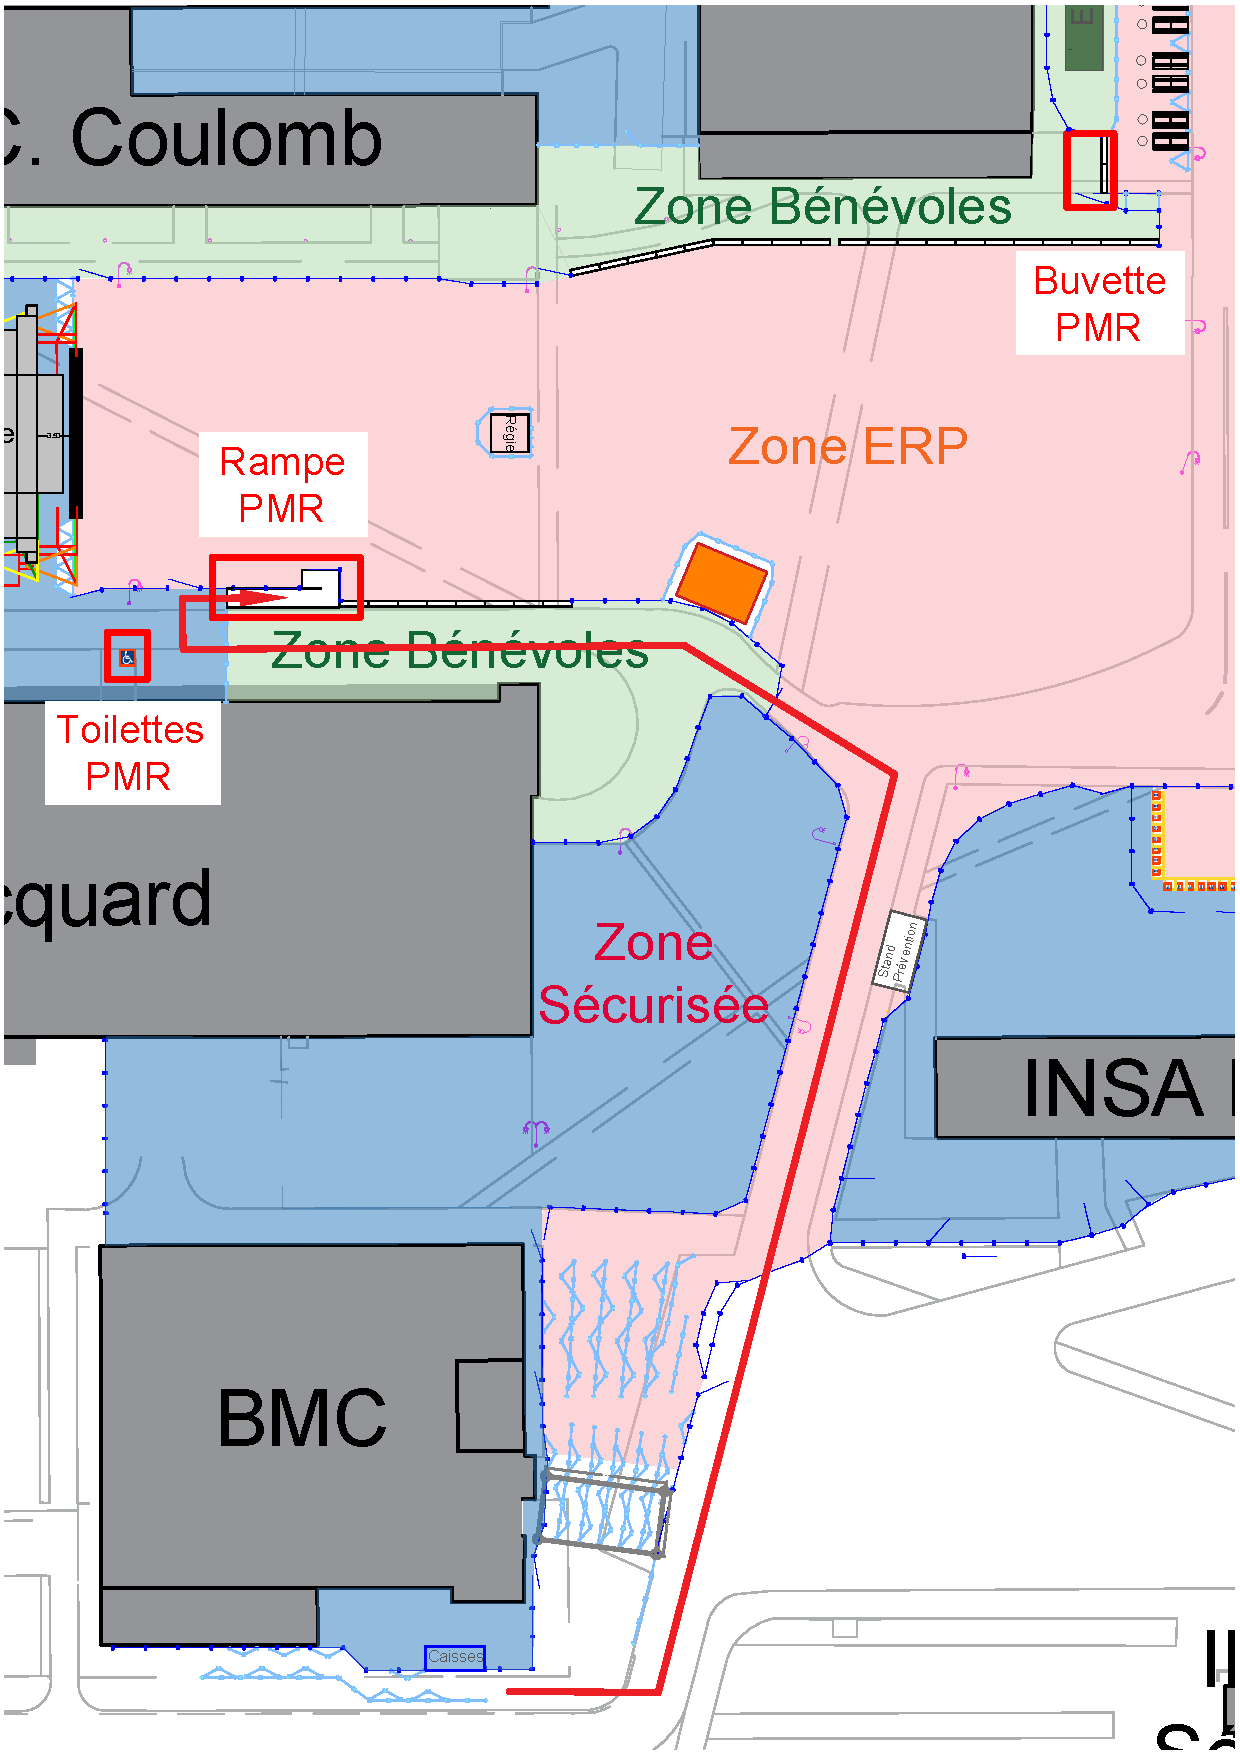
\includegraphics[width=.45\textwidth, trim=0 0 0 30,clip]{Exports/Plan_24h_44eme-PMR_sud}\\
\end{tabular}

\end{frame}

%========================================
%PREVENTION SUR LE CAMPUS
%========================================

\section{Prévention sur le campus}

\begin{frame}

\centering\Huge{\textbf{Prévention sur le campus}}

\end{frame}

\begin{frame}

\frametitle{Dispositions concernant le campus}
\begin{itemize}
\item Services médicaux et de sécurité civile à proximité :
\begin{itemize}
\item \textbf{Services de police autorisés à intervenir} sur le campus
\item \textbf{Pompiers} informés
\item Proximité de la \textbf{clinique du Tonkin} 
\end{itemize}
\item Bâtiments et laboratoires : 
\begin{itemize}
\item \textbf{Renforcement} du Service de Prévention et de sécurité de l’INSA (4 agents supplémentaires)
\item \textbf{Renforcement} du Service de Prévention et de sécurité de l’UCBL (2 agents supplémentaires)
\item Astreinte de la Direction du Patrimoine de l’INSA \textbf{doublée} (technique et électrique)
\end{itemize}
\end{itemize}

\end{frame}

\begin{frame}

\frametitle{Transports en commun}
\begin{itemize}
\item Mesures de prévention :
\begin{itemize}
\item Blocage des emplacements dangereux
\item Agents de sûreté en fin de soirée aux abords des stations de tramway
\end{itemize}
\item Contact avec le PC sécurité TCL:
\begin{itemize}
\item En cas d’évacuation 
\end{itemize}
\item Réunion avec Keolis - Sytral le 3 avril au sujet du stockage temporaire des rames sur le campus
\begin{itemize}
\item 20 rames seront stockées en dehors du dépot
\item Des agents de surêté TCL seront chargés de la surveillance du matériel
\end{itemize}
\end{itemize}

\end{frame}

\begin{frame}

\frametitle{Protection des bâtiments sur le campus}

\centering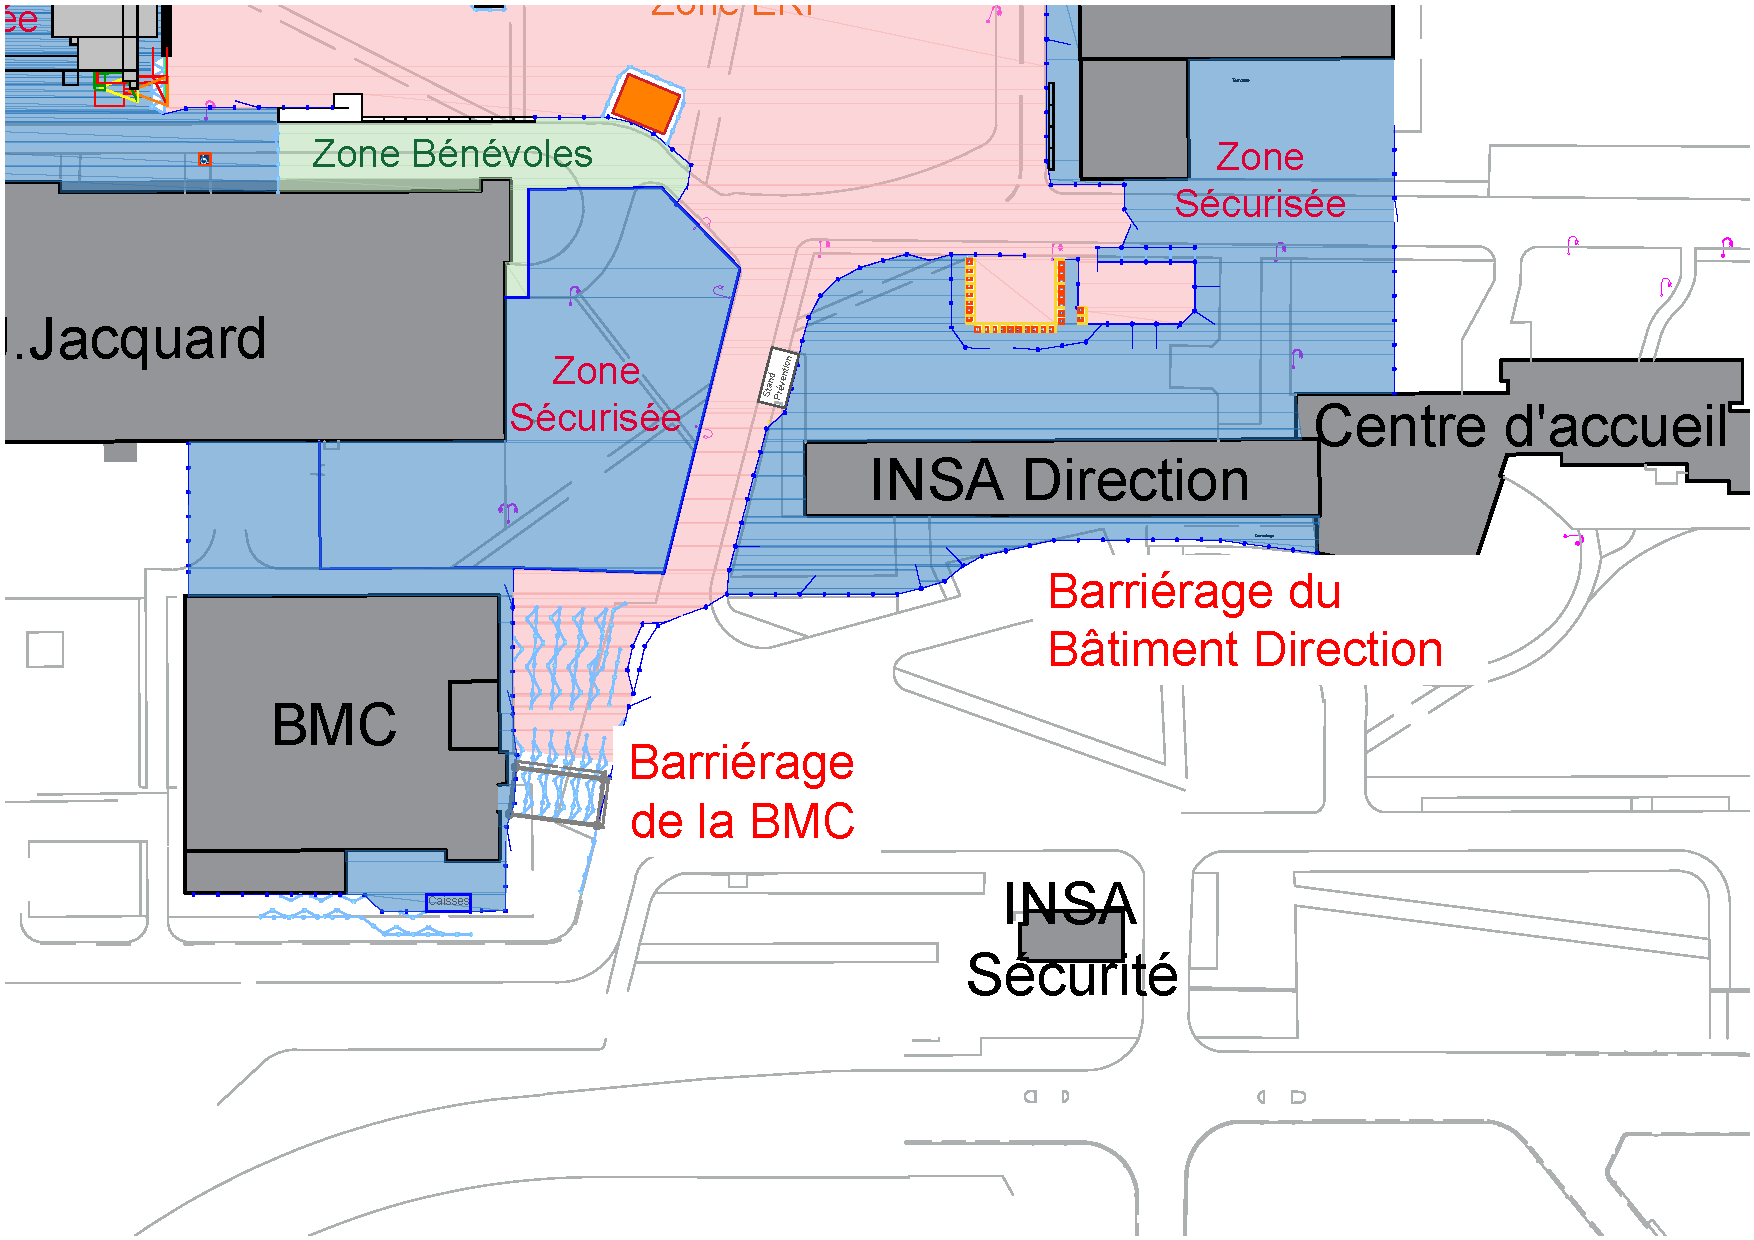
\includegraphics[width=.9\textwidth, trim=0 0 0 0,clip]{Exports/Plan_24h_44eme-Protection_Bat}

\end{frame}

\begin{frame}

\frametitle{Avant la manifestation}
\begin{itemize}
\item Rappel des précautions à prendre en raison de l’affluence exceptionnelle :
\begin{itemize}
\item Bien fermer les logements et locaux
\item Faire attention aux vols à la tire	
\end{itemize}
\item Pose d’affiches de sensibilisation sur les supports d’affichage du campus et dans les résidences. 
\item Communication par voie électronique à l’ensemble des étudiants et personnels.
\item Désactivation des badges d’accès aux bâtiments (de cours \& laboratoires) et des ascenseurs.
\end{itemize}

\end{frame}

\begin{frame}

\frametitle{Pendant la manifestation}
\begin{itemize}
\item Présence d’organismes de prévention :
\begin{itemize}
\item Avenir Santé – Génération Cobayes
\end{itemize}
\item Thèmes abordés :
\begin{itemize}
\item Alcool, drogues
\item Sécurité routière (opération SAM)
\item Sexualité, IST
\item Comportements à risques
\end{itemize}
\item Equipes mobiles pendant les concerts
\item Diffusion de messages de prévention sur les écrans de la scène
\end{itemize}

\end{frame}

\begin{frame}

\frametitle{Emplacement du stand de prévention}
\centering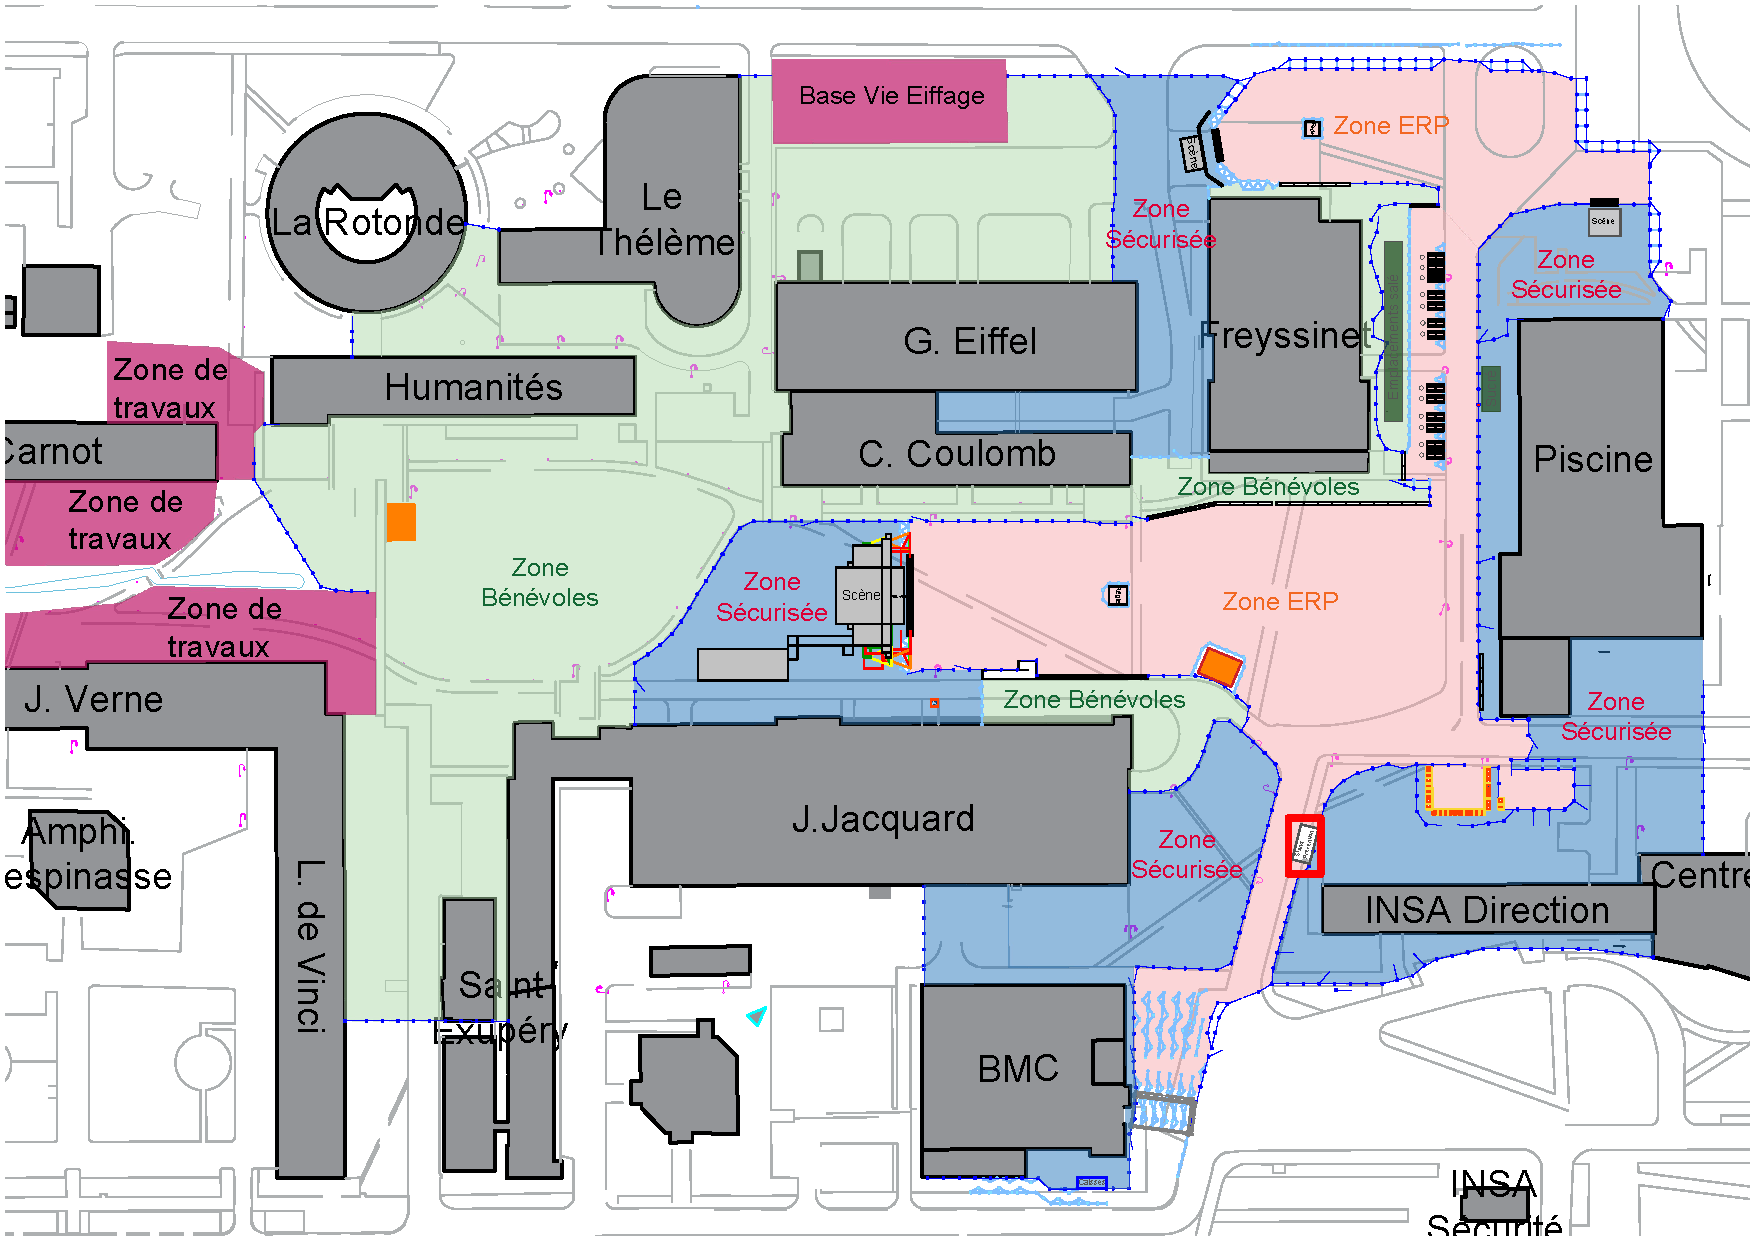
\includegraphics[height=.9\textheight, trim=350 0 0 100,clip]{Exports/Plan_24h_44eme-Stand_prevention}

\end{frame}

\begin{frame}

\frametitle{Dispositions spécifiques au CETIAT}
\begin{tabular}{i{.35\textwidth} c}
\item Centre technique situé sur l'avenue des Arts
\vspace{1mm}
\item Stockage de divers matériaux \textbf{inflammables}
\vspace{1mm}
\item Gardiennage le vendredi, samedi de 20h à 4h et dimanche soir de 20h à 23h30
\vspace{1mm}
\item Liaison radio permanente avec le PC sécurité
& 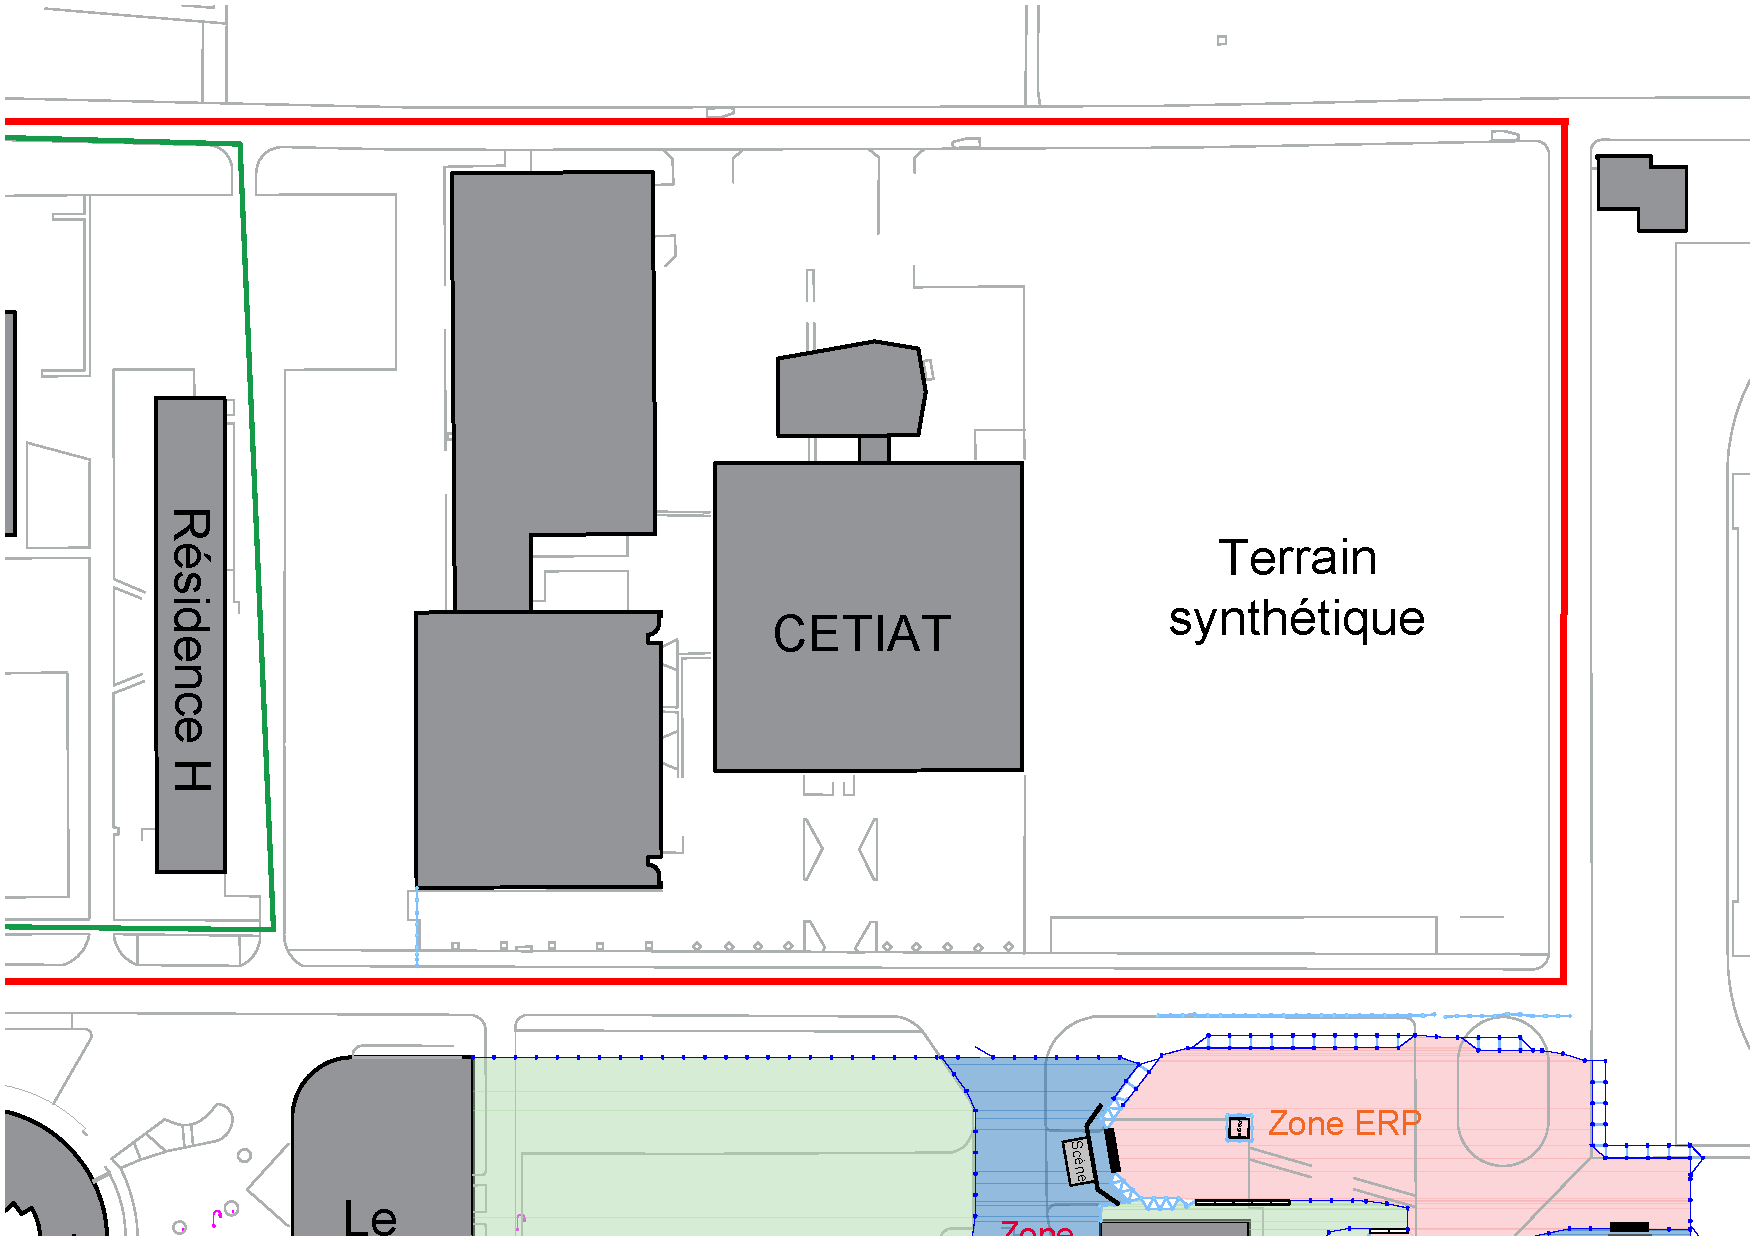
\includegraphics[width=.6\textwidth, trim=100 0 100 30,clip]{Exports/Plan_24h_44eme-CETIAT}\\
\end{tabular}

\end{frame}

%========================================
%COURSES ET ANIMATIONS
%========================================

\section{Courses et animations}

\begin{frame}

\centering\Huge{\textbf{Courses et animations}}

\end{frame}

\begin{frame}

\frametitle{Course cylcliste et à pied}
\begin{tabular}{i{.4\textwidth} i{.5\textwidth}}
\item \textbf{3 points} de passage
\item \textbf{2 organisateurs} avec chasuble par point de passage
& \item Rondes régulière en \textbf{voiture-balai}
\item Véhicule de la \textbf{Croix-Rouge} présent avec \textbf{3 secouristes} pendant la durée de la course
\end{tabular}
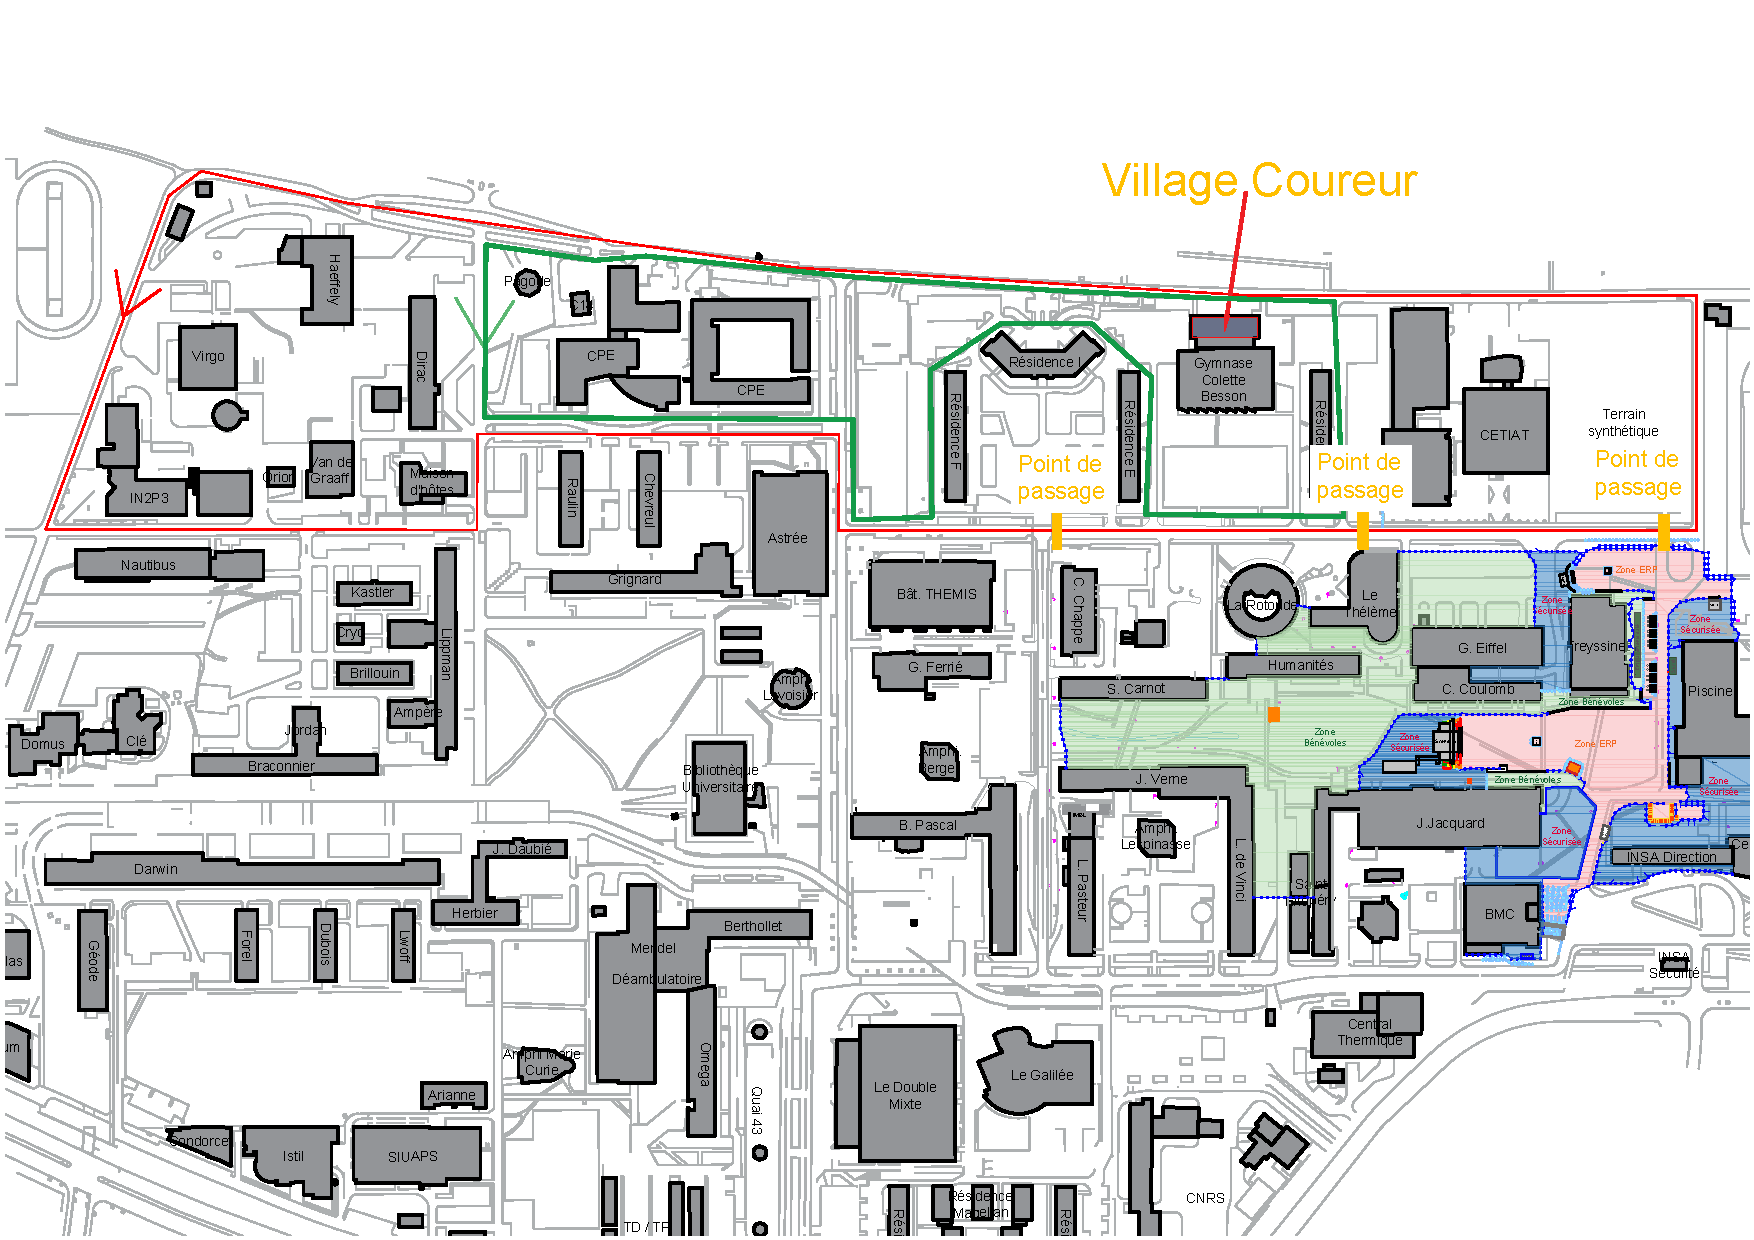
\includegraphics[width=\textwidth, trim=0 300 0 0,clip]{Exports/Plan_24h_44eme-Parcours_courses}

\end{frame}

\begin{frame}

\frametitle{Course cycliste et à pied}
\begin{itemize}
\item \textbf{Risques :}
\begin{itemize}
\item Chutes (fatigue, vitesse)
\item Collisions avec les spectateurs
\end{itemize}
\item \textbf{Mesures préventives :}
\begin{itemize}
\item \textbf{Port du casque} et éclairage de vélo obligatoires 
\item \textbf{Vérification} des certificats médicaux / Licences Sportives
\item \textbf{Barrièrage} et signalisation des points sensibles
\item \textbf{Points de passage surveillés} pour les spectateurs
\item Équipe de \textbf{secouristes} présente sur le parcours
\item \textbf{Surveillance} constante par une voiture balai
\item \textbf{Éclairage} de la course pendant la nuit
\end{itemize}
\end{itemize}
\end{frame}

\begin{frame}

\frametitle{Animations}
\begin{itemize}
\item Environ \textbf{60 animations} regroupées en 3 pôles
\item Horaires : \textbf{10h-18h} les 19 et 20 mai
\item \textbf{3 responsables animations} en liaison radio avec le PC sécurité
\end{itemize}
\begin{tabular}{i{.35\textwidth} c}
\item \textbf{Patrouilles} d'agents de sûreté
\item Agents de sûreté \textbf{fixes} aux points sensibles
\vspace{1.5cm}
& 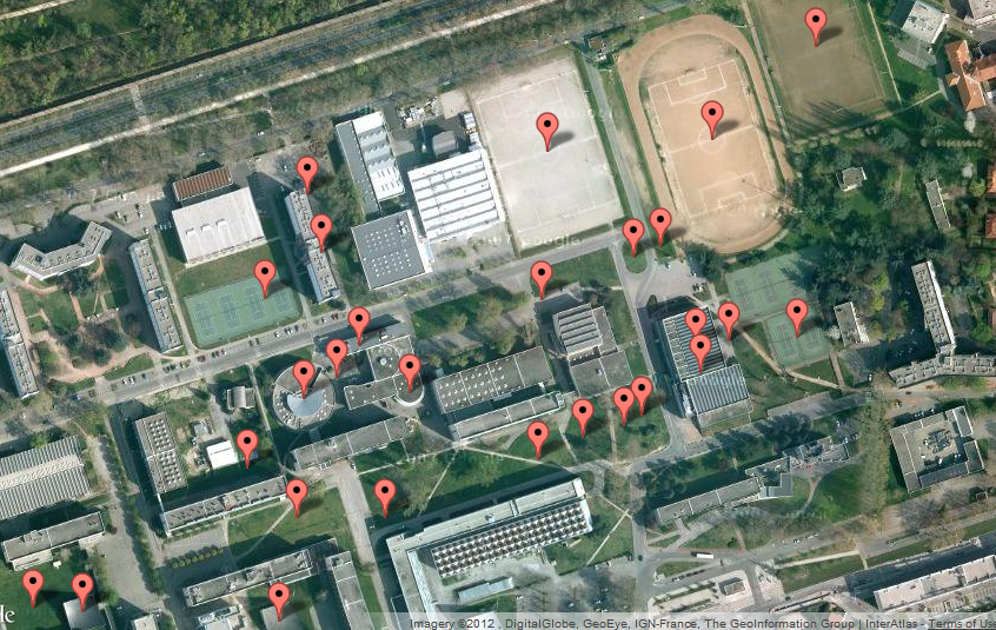
\includegraphics[width=.6\textwidth, trim=0 0 0 0,clip]{Images/animations}\\
\end{tabular}


\end{frame}

\begin{frame}

\frametitle{Répartition des AS en journée}
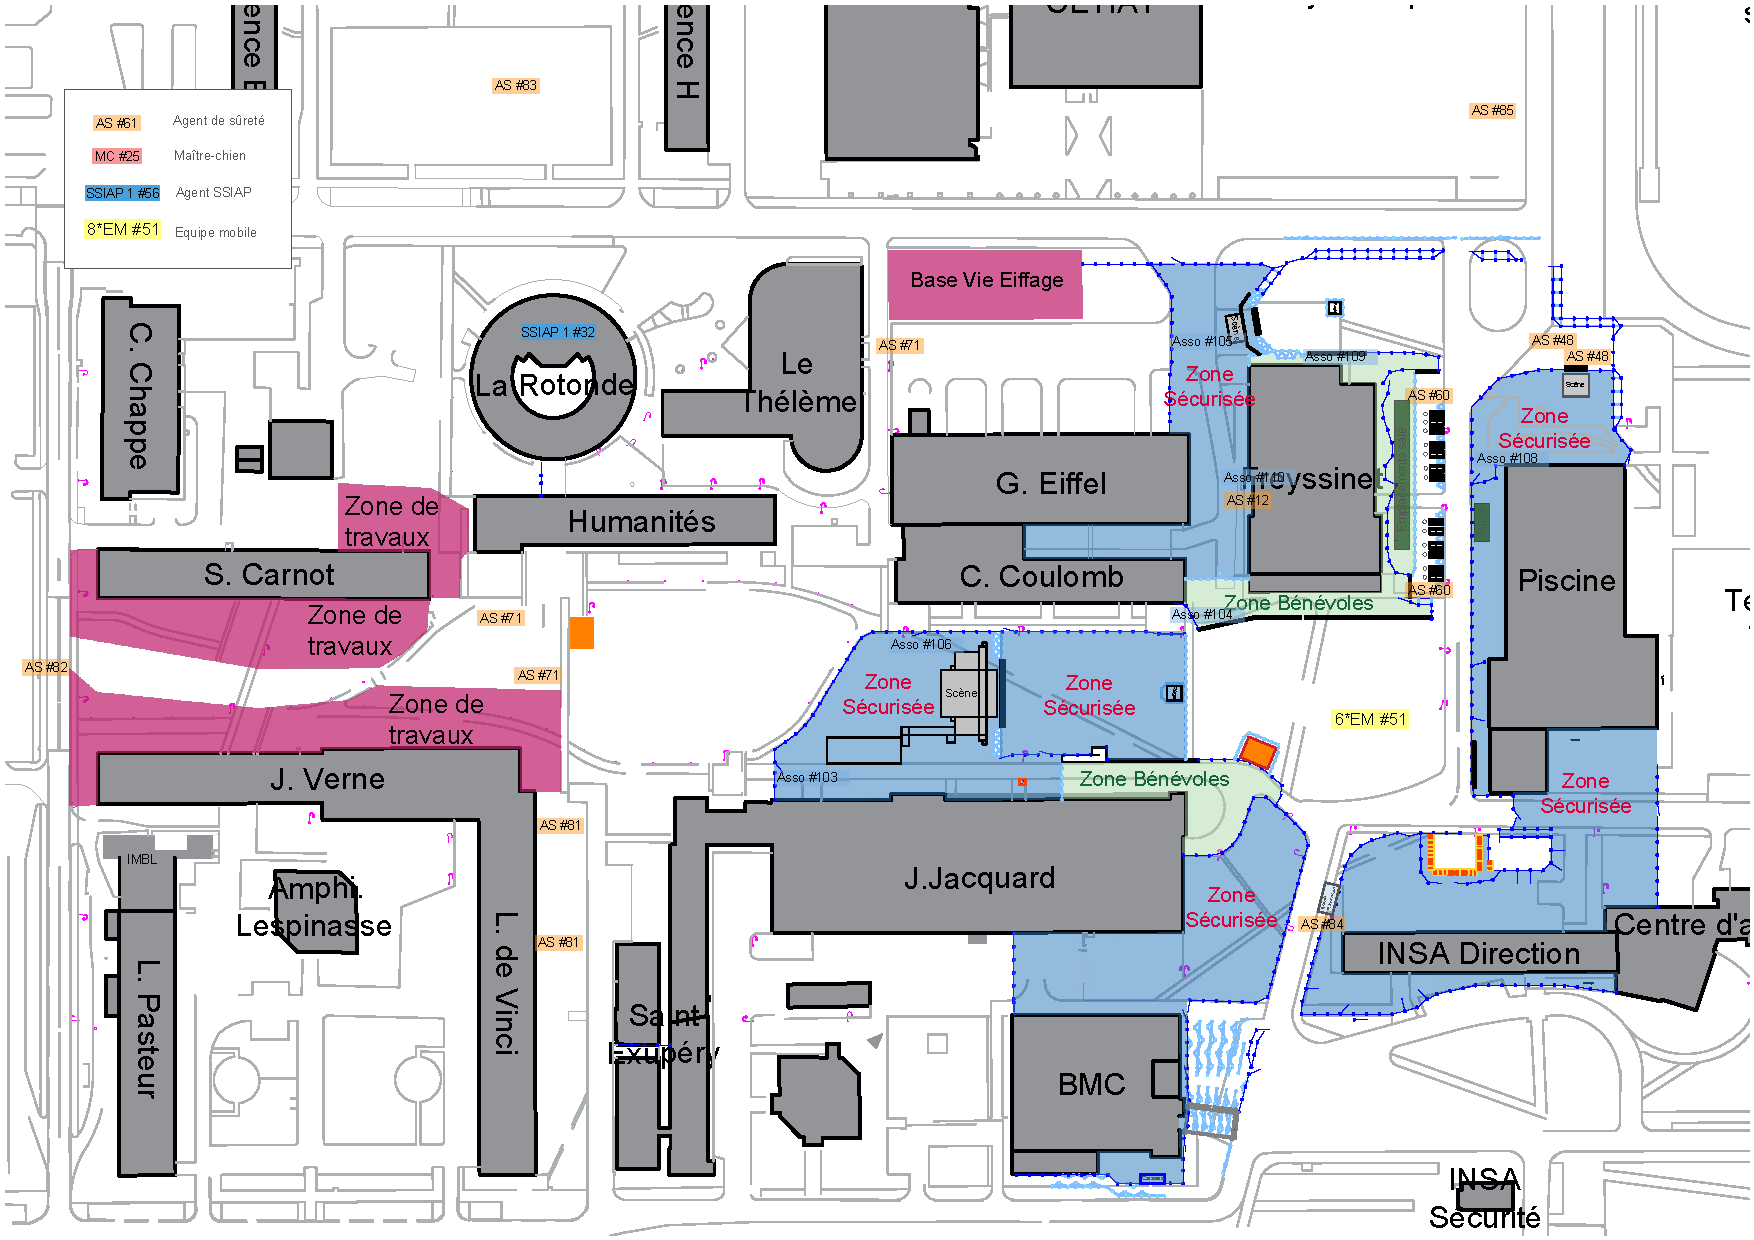
\includegraphics[width=\textwidth, trim=0 0 0 30,clip]{Exports/Plan_24h_44eme-AS_Jour}

\end{frame}

\begin{frame}

\frametitle{Animations sensibles}
\begin{itemize}
\item Feu d’artifice  / Spectacle de feu
\item Animation Phare : Tyrolienne
\item Dispositif de protection spécifique :
\begin{itemize}
\item Barrièrage de la zone 
\item Agents de sûreté dédiés
\item Extincteurs
\end{itemize}
\end{itemize}

\end{frame}

\begin{frame}

\frametitle{Animations sensibles - Feu d'artifice}
\begin{itemize}
\item \textbf{Spectacle de feu}
\begin{itemize}
\item Même emplacement que le feu d’artifice 
\item 10 mètres de séparation avec le public
\item Spectacle le 20 mai à 22h30
\end{itemize}
\item \textbf{Feu d’artifice}
\begin{itemize}
\item Type K4
\item 17,48 kg de matière active 
\item 95 mètres de séparation avec le public
\item Tir le \textbf{20 mai à 23h00}
\item Société ShowTechnic, comme les années précédentes
\item Public : environ 500 personnes
\end{itemize}
\end{itemize}

\end{frame}

\begin{frame}

\frametitle{Tyrolienne}
\begin{tabular}{i{.37\textwidth} c}
\item Prestataire \textbf{agréé}
\vspace{1mm}
\item Animation \textbf{certifiée}
\vspace{1mm}
\item Zone délimitée par des \textbf{barrières}
\vspace{1mm}
\item \textbf{Agent de sûreté} présent pendant l'exploitation
\vspace{1mm}
\item 8m de haut pour 40m de long
\vspace{1mm}
\item Encadrant BE
\vspace{.5cm}
& 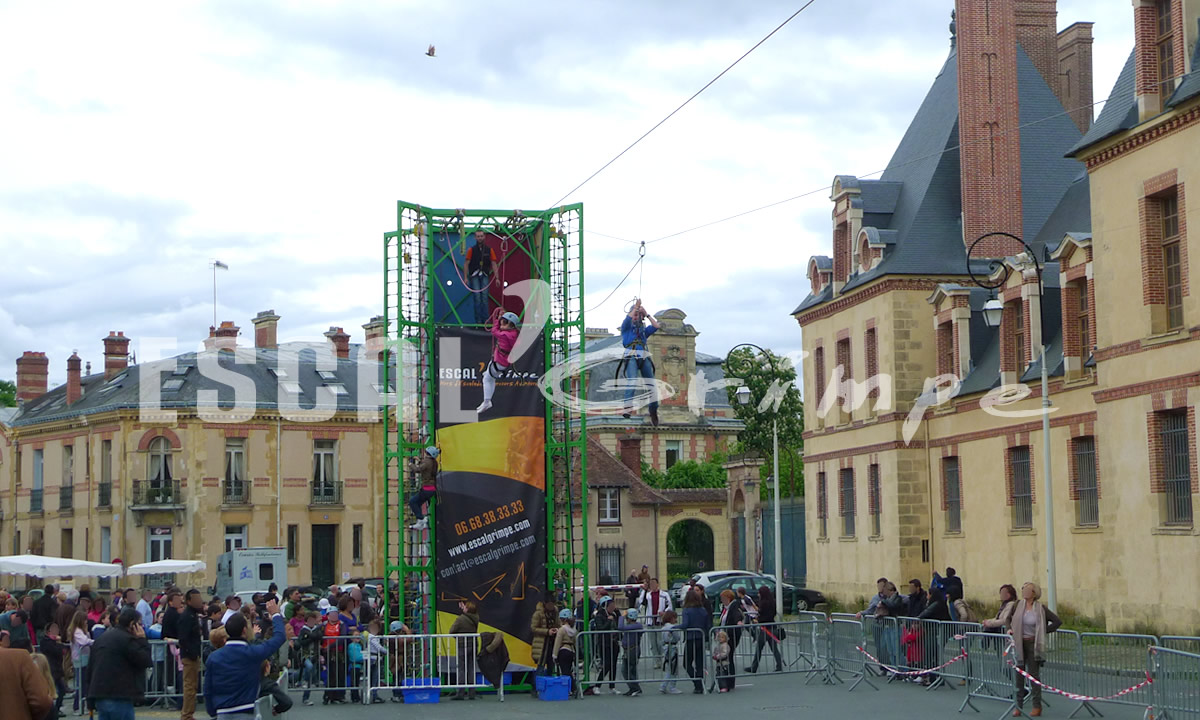
\includegraphics[width=.6\textwidth, trim=130 0 280 0,clip]{Annexes/Images/tyrolienne}\\
\end{tabular}

\end{frame}

\begin{frame}

\frametitle{Soirée du dimanche}
\begin{tabular}{i{.35\textwidth} c}
\item Dimanche 20 mai de \textbf{20h à 22h30}
\vspace{.3cm}
\item Concerts de \textbf{jazz}
\vspace{.3cm}
\item Communication \textbf{réduite}
\vspace{.3cm}
\item Mise en place d'une \textbf{zone ERP réduite}
\vspace{2cm}
& 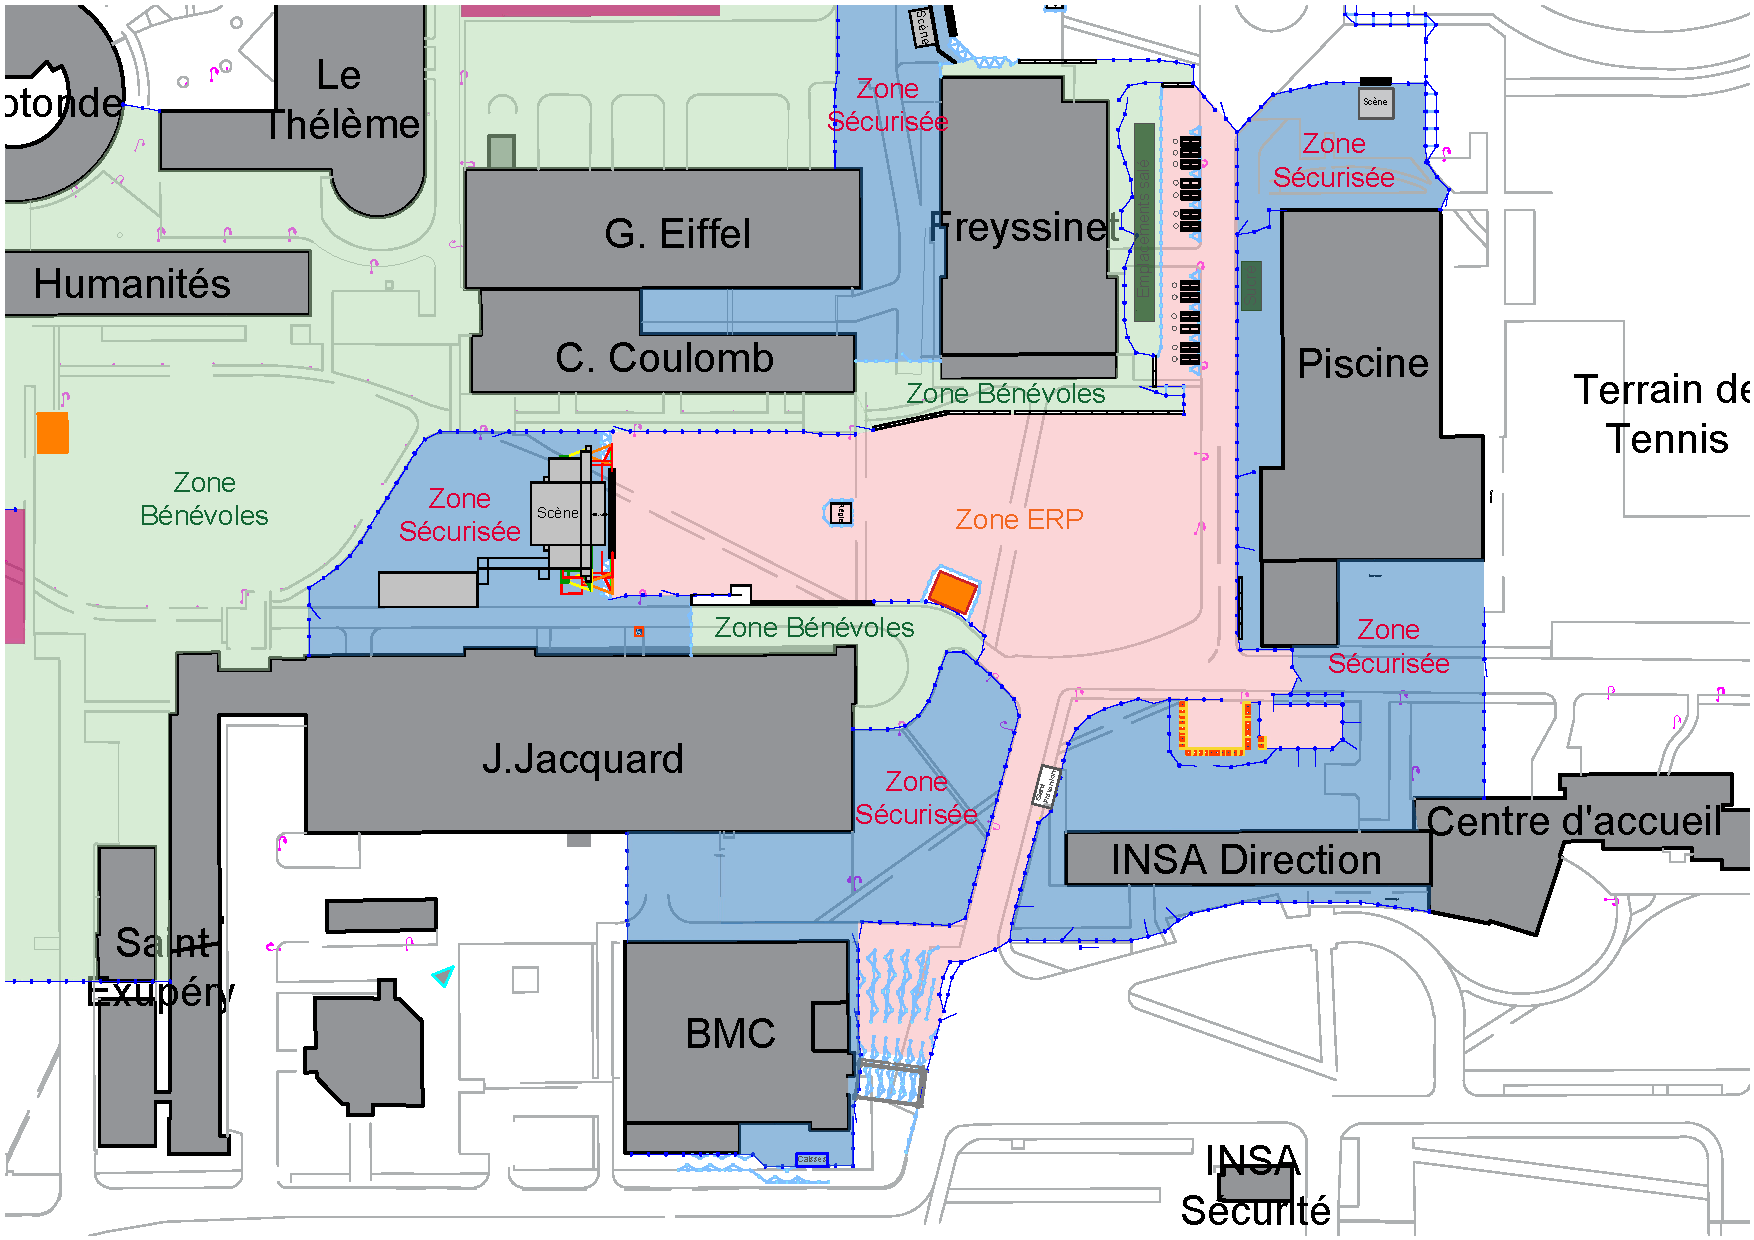
\includegraphics[width=.6\textwidth, trim=200 0 170 30,clip]{Exports/Plan_24h_44eme-ERP_Dimanche}\\
\end{tabular}

\end{frame}

\begin{frame}

\frametitle{Soirée du dimanche}
\begin{tabular}{i{.4\textwidth} c}
\item Exploitation : \textbf{2 000 personnes} (décompte à l'entrée)
\item \textbf{6 sorties et 60 UP}
\item Dispositions des soirées du vendredi et samedi conservées
\item Blocs phares en cas de coupure
\item Palpations aux entrées
\item \textbf{Agents de sûreté} répartis sur la zone (dont \textbf{agents SSIAP})
& 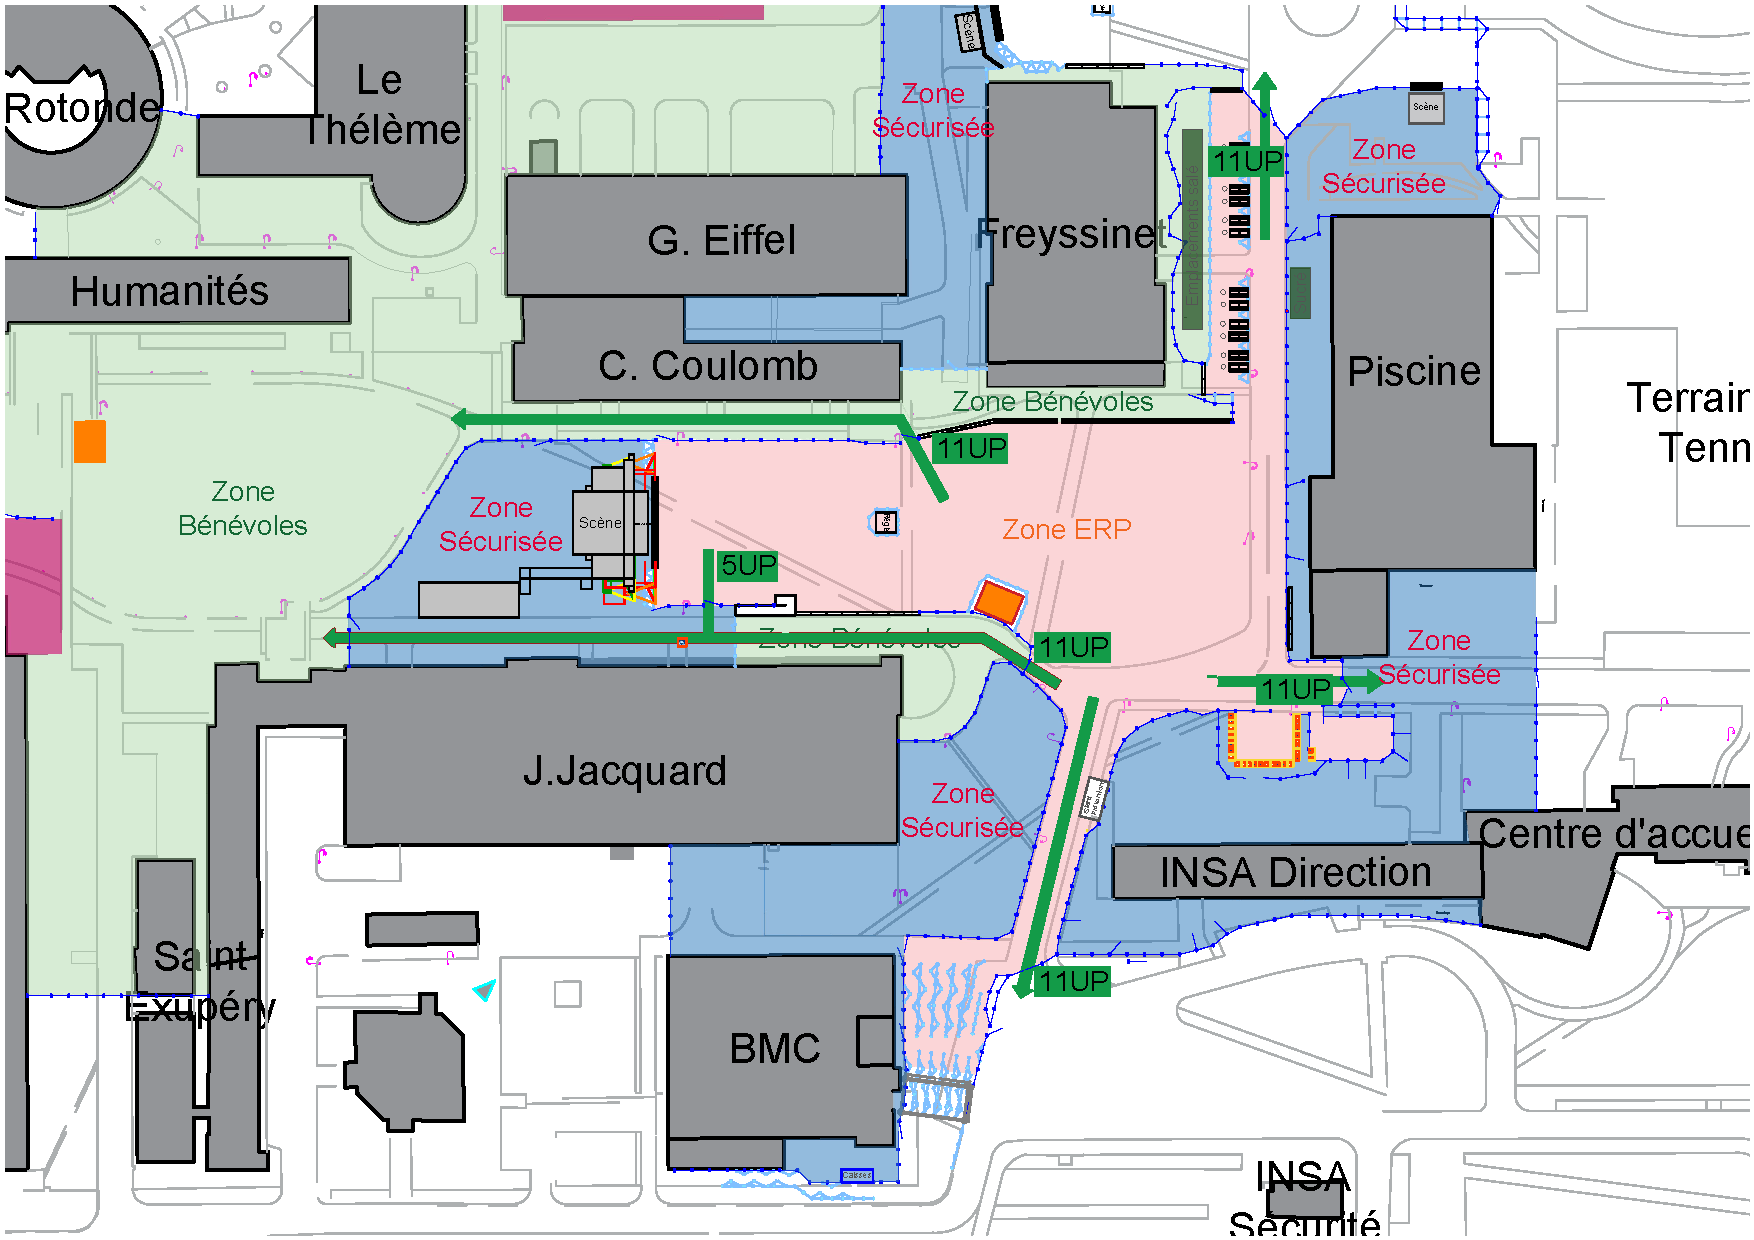
\includegraphics[width=.55\textwidth, trim=200 0 170 30,clip]{Exports/Plan_24h_44eme-Dimanche_IS}\\
\end{tabular}

\end{frame}

%========================================
%CIRCULATION SUR LE CAMPUS
%========================================

\section{Circulation sur le campus}

\begin{frame}

\centering\Huge{\textbf{Circulation sur le campus}}

\end{frame}

\begin{frame}

\frametitle{Contexte}
\begin{itemize}
\item Risque accru d'attentat
\item Recours au véhicule-bélier fréquent
\item Sécurisation de la course
\item Forte affluence de piéton
\end{itemize}
\vspace{1cm}
\textbf{$\rightarrow$  Nécessité de maitriser la circulation sur le campus}\\
\vspace{1cm}
\textbf{$\rightarrow$  Arrêtés municipaux demandés à la mairie}

\end{frame}

\begin{frame}

\frametitle{Dispositif en journée (1/2)}
\begin{itemize}
\item Campus \textbf{fermé à la circulation} du vendredi 18h au dimanche 23h59
\item Mise en place de \textbf{points de contrôle}
\item Distributions de\textbf{ laissez-passer} à l'avance
\end{itemize}
\centering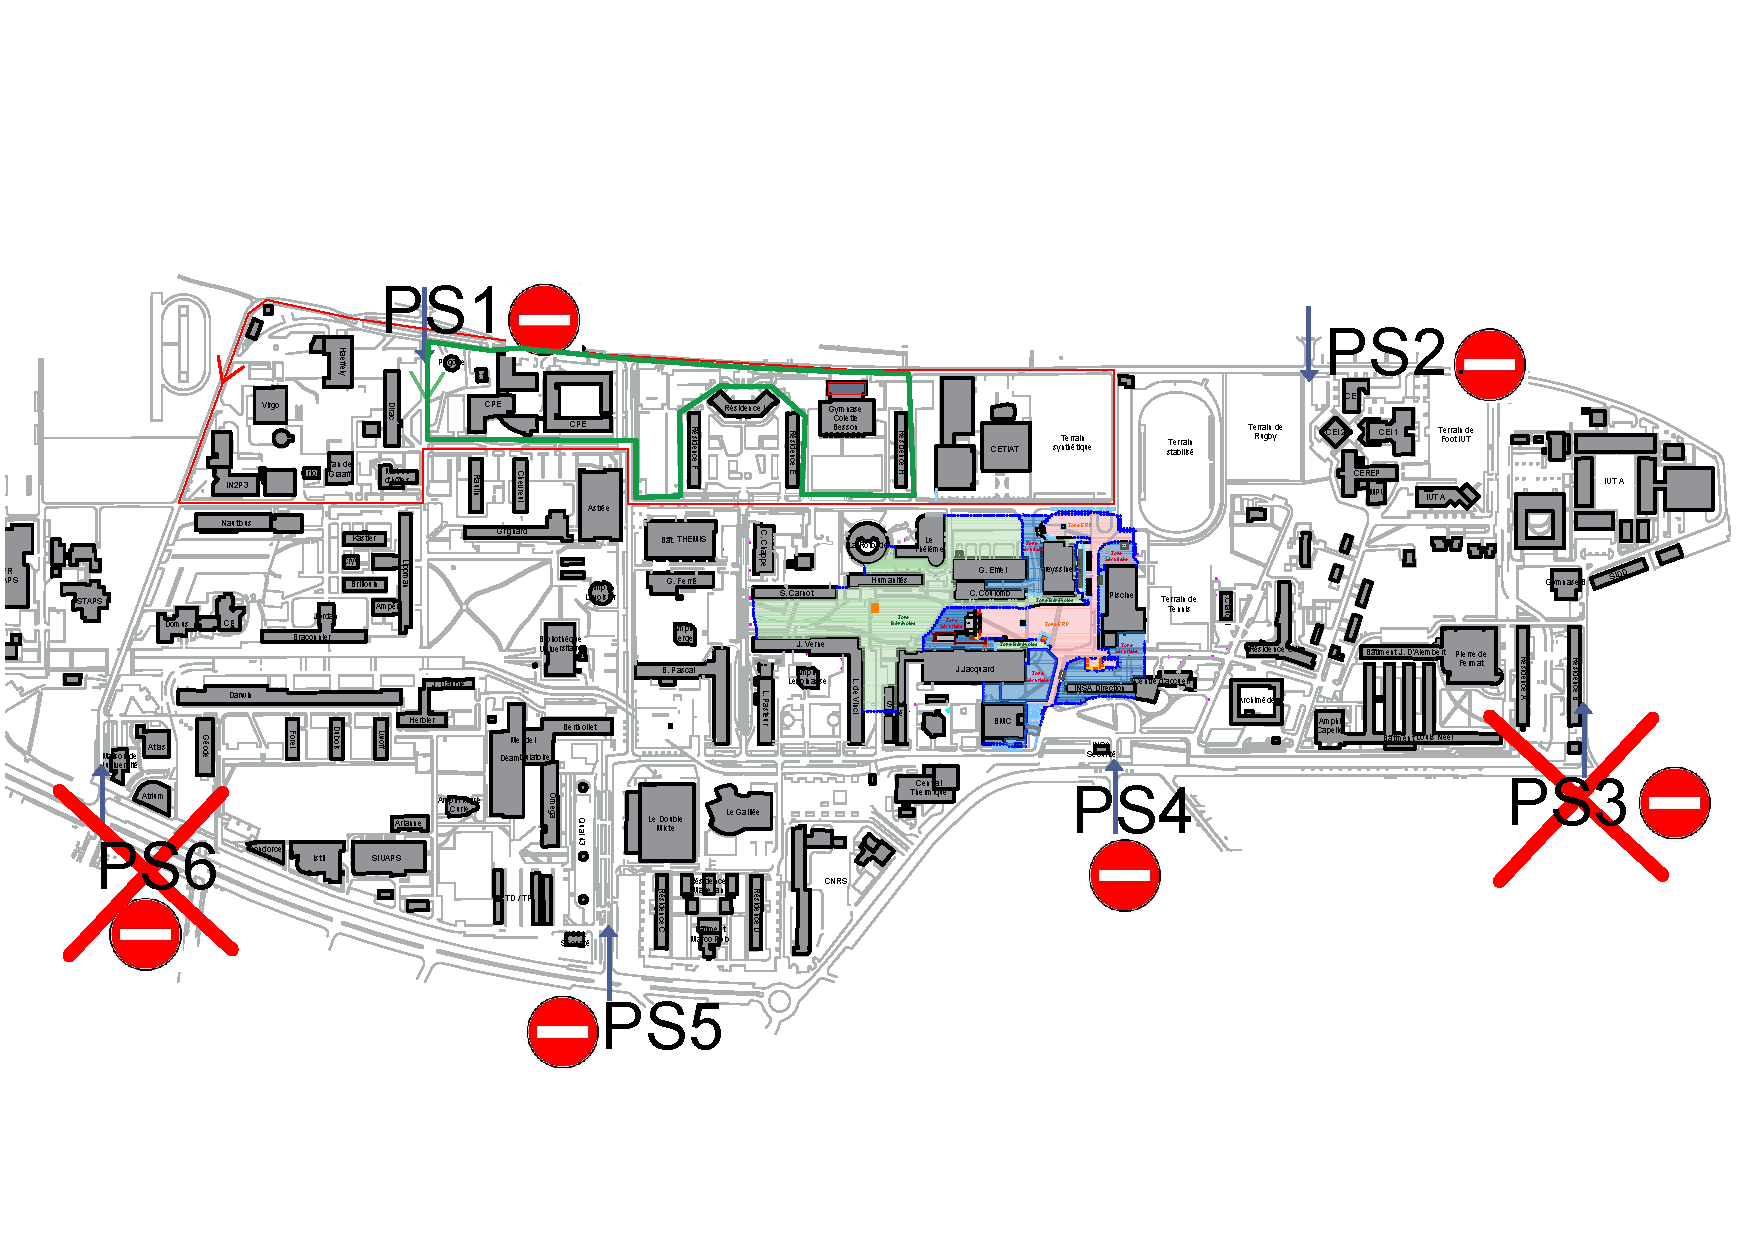
\includegraphics[width=\textwidth, trim=0 0 0 100,clip]{Exports/Plan_24h_44eme-Points_Secu}

\end{frame}

\begin{frame}

\frametitle{Dispositif en journée (2/2)}
\begin{itemize}
\item \textbf{6 points} d'accès au campus
\item 2 points \textbf{condamnés} par des blocs en béton
\item Binômes de bénévoles pour \textbf{vérifier les laissez-passer}
\item Liaison radio avec le \textbf{PC Sécurité}
\end{itemize}
\centering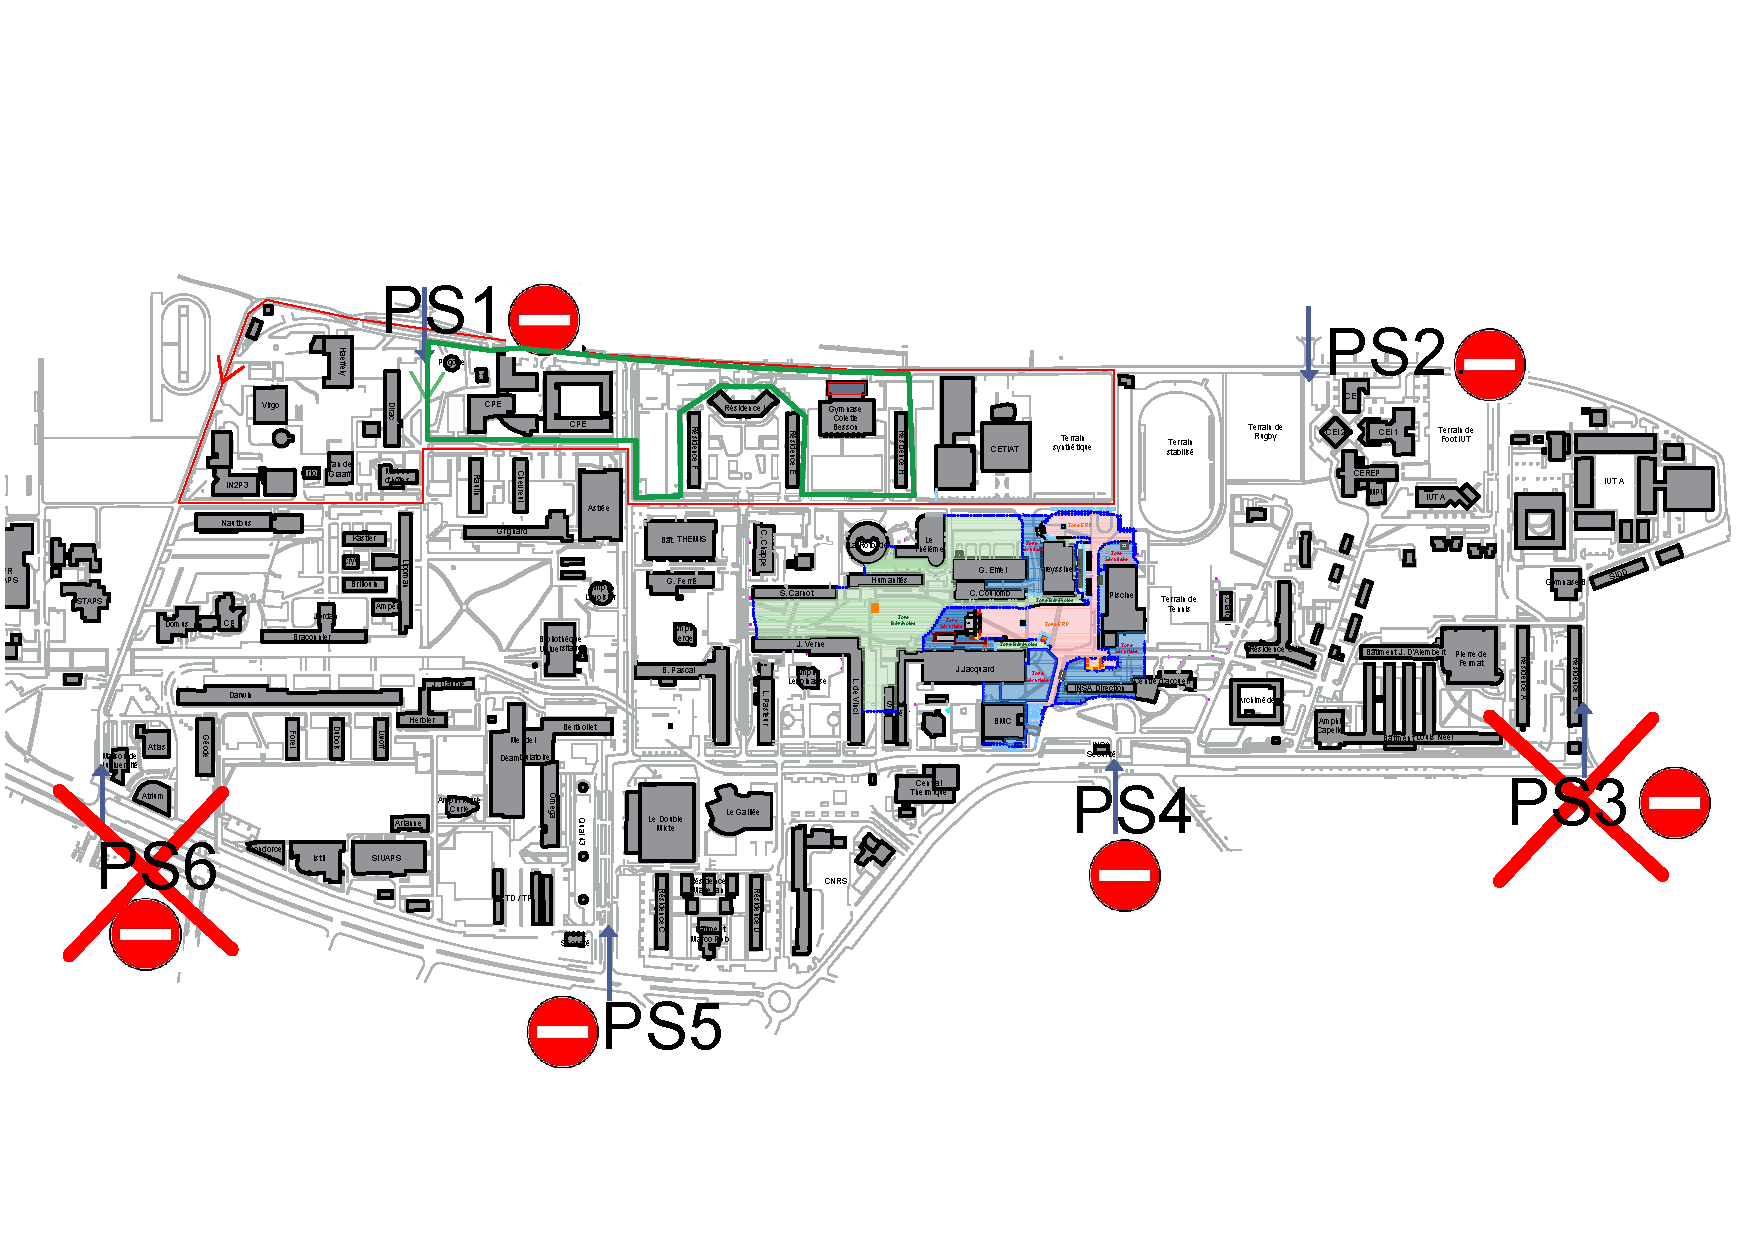
\includegraphics[width=\textwidth, trim=0 0 0 100,clip]{Exports/Plan_24h_44eme-Points_Secu}

\end{frame}

\begin{frame}

\frametitle{Dispositif en soirée (1/2)}
\begin{itemize}
\item \textbf{Renforcement} du "dispositif journée" entre 20h et 5h les vendredi et samedi soir
\item Remplacement des bénévoles par un \textbf{agent de sûreté}
\item Présence d'un véhicule en \textbf{travers de la route}
\item Blocs en béton et barrières aux alentours pour empêcher un contournement
\item \textbf{Restriction} très forte de la circulation (même avec laissez-passer)
\end{itemize}
\centering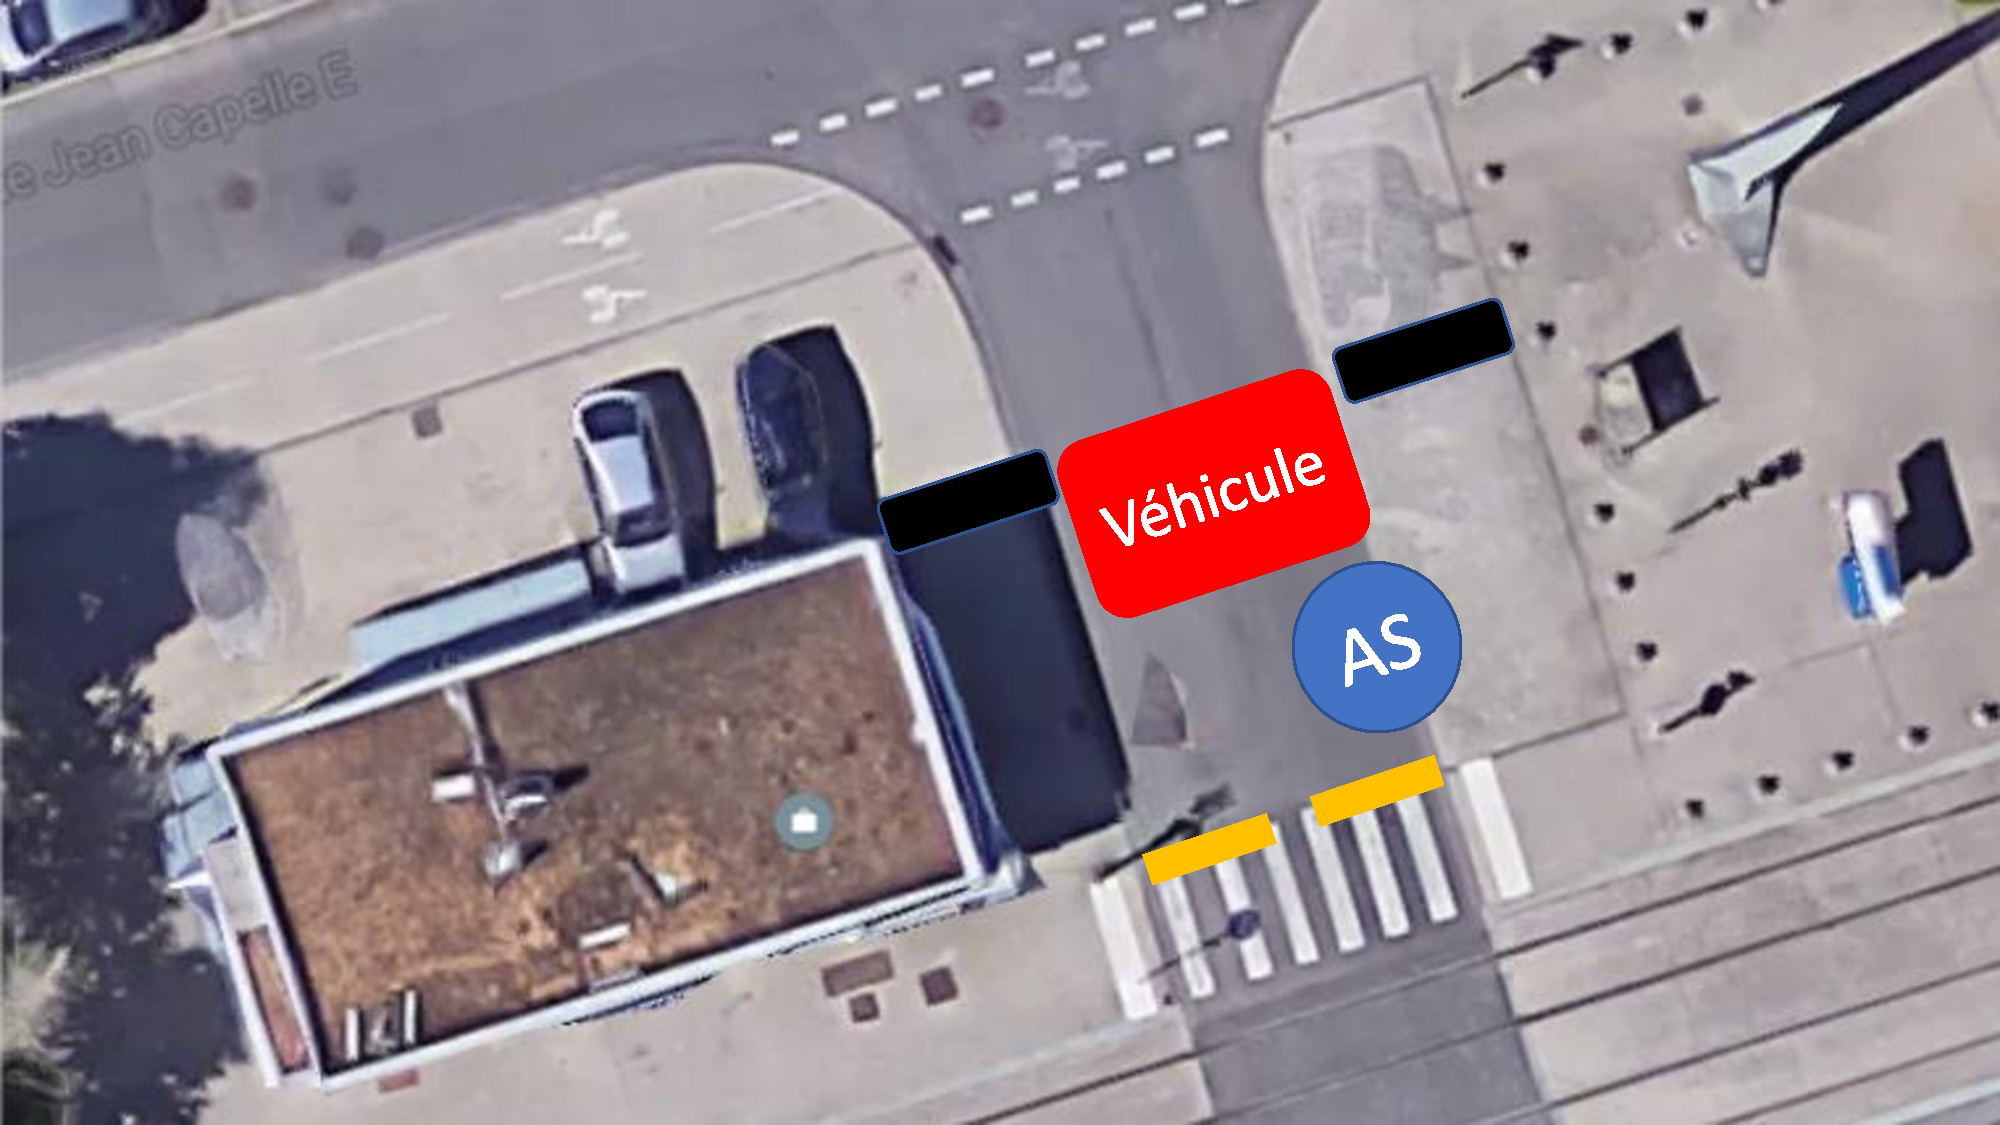
\includegraphics[width=.6\textwidth, trim=0 0 0 0,clip]{Images/PS}

\end{frame}

\begin{frame}

\frametitle{Dispositif en soirée (2/2)}
\begin{itemize}
\item Deuxième \textbf{périmètre de sécurité}
\item \textbf{Protection supplémentaire} pour la zone à forte affluence
\item Véhicules gardés \textbf{en continu}
\end{itemize}
\centering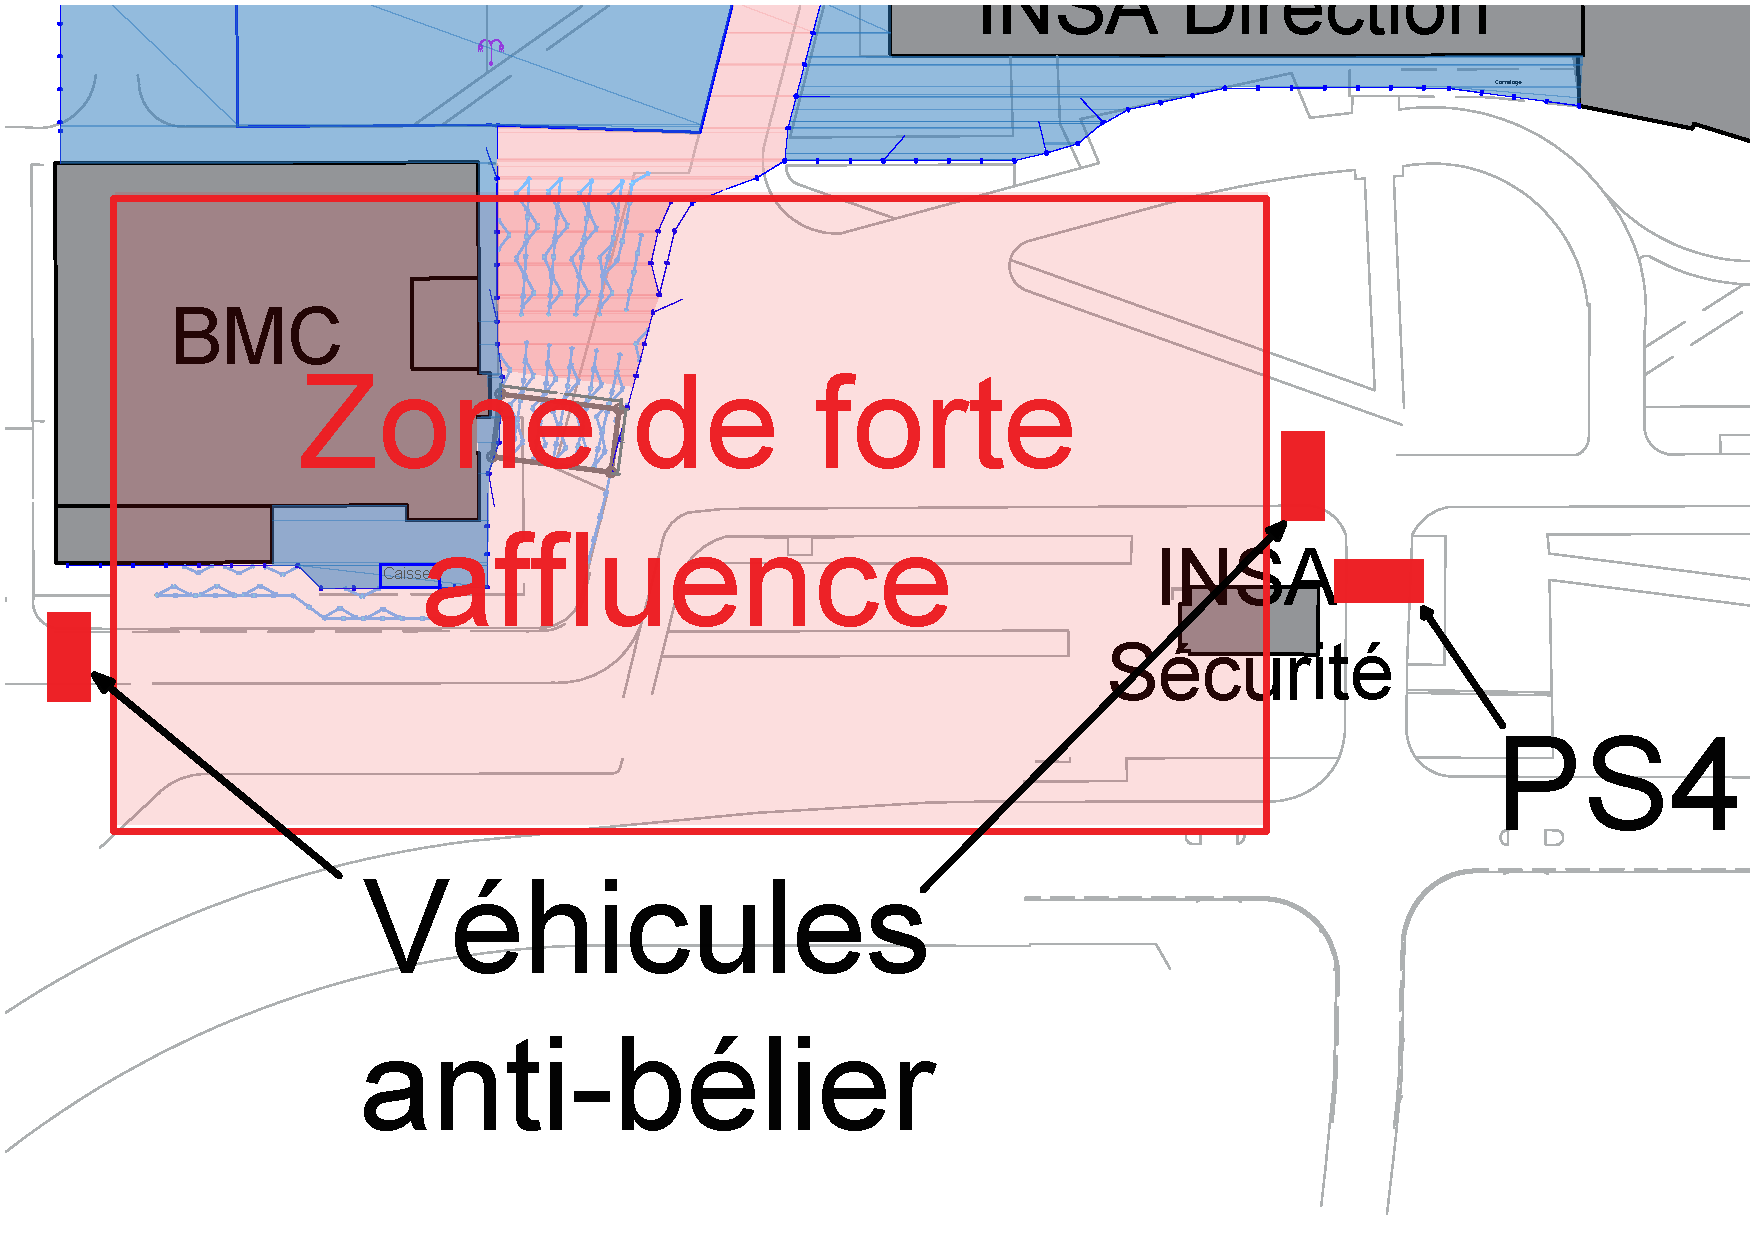
\includegraphics[width=.8\textwidth, trim=0 0 0 0,clip]{Exports/Plan_24h_44eme-Vehicules_beliers}

\end{frame}

\begin{frame}

\frametitle{Véhicules autorisés à circuler la nuit}
Les vendredi et samedi de 20h à 5h, seuls les véhicules suivants pourront être autorisés à entrer sur le campus :
\begin{itemize}
\item Secours (Police, pompiers, Croix-Rouge, etc.)
\item Les services prévention \& sécurité INSA/UCBL
\item Certains véhicules organisateurs
\item Les PMR munis d’un justificatif en cours de validité
\item Personnel d’astreinte INSA \& UCBL
\item Agents TCL prenant leur service
\end{itemize}
\textbf{Les autres laissez-passer ne seront pas autorisés.}


\end{frame}

\begin{frame}

\frametitle{Laissez-passer}
\begin{itemize}
\item \textbf{Le laissez-passer est} :
\begin{itemize}
\item Nominatif et incessible
\item Valable durant des plages horaires spécifiques
\item Valables pour certains points d’accès uniquement
\end{itemize}
\item \textbf{Lors du contrôle} :
\begin{itemize}
\item L’identité du conducteur sera vérifiée
\item L’authenticité du laissez-passer pourra être vérifiée auprès du PC Sécurité en cas de doute
\end{itemize}
\end{itemize}

\end{frame}

\begin{frame}

\frametitle{Parking pour le personnel de l'INSA}
\vspace{.5cm}
Mise à disposition d’un parking extérieur au campus pour les personnels logés.


\centering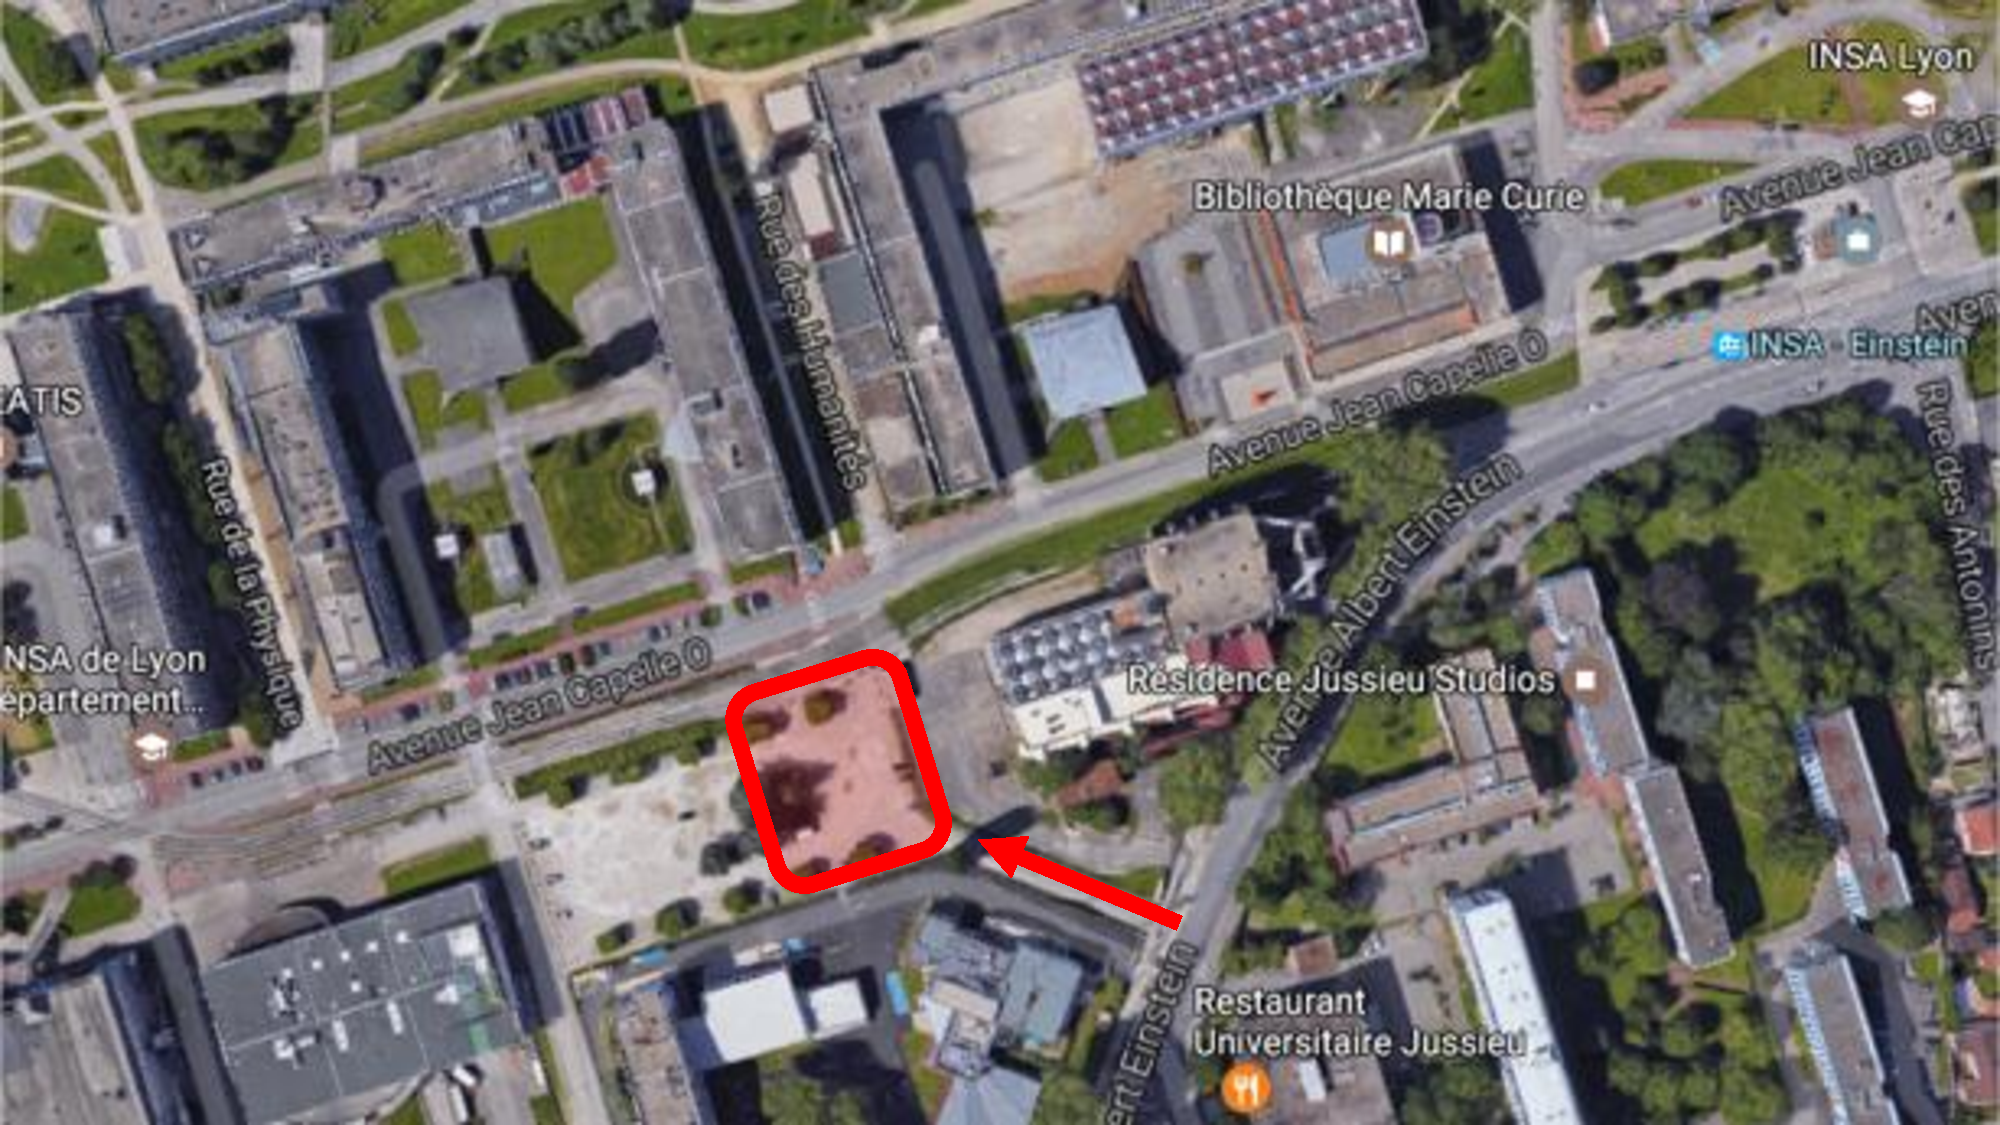
\includegraphics[width=.8\textwidth, trim=0 0 0 0,clip]{Images/parking_personnel}

\end{frame}
%
%\begin{frame}
%
%\frametitle{Communication}
%\begin{itemize}
%\item S-4 : mail au personnel logé + astreinte pour demande de laissez-passer (formulaire à remplir)
%\item S-4 : mail d’information aux usagers du campus
%\item S-2 : mail envoyé aux résidences E, F, H et I de l’INSA (ciblé sur les courses)
%\item S-2 : affichage dans les résidences de l’INSA
%\item S-1 : rappel du dispositif aux usagers
%\item De S-2 jusqu’à l’événement, flyage des véhicules au niveau des zones concernées
%\end{itemize}
%
%\end{frame}

\begin{frame}

\frametitle{Signalisation}
\begin{itemize}
\item Panneaux d’interdiction de stationner
\vspace{2mm}
\item Panneaux déviation pour les PS condamnés
\vspace{2mm}
\item Mise à disposition d’un parking accessible depuis l’extérieur pour les personnels
\end{itemize}

\end{frame}

\section{Conclusion}

\begin{frame}

\centering\Huge{\textbf{Conclusion}}

\end{frame}

\begin{frame}

\frametitle{Conclusion}
\begin{itemize}
\item Nouvelles infrastructures scéniques
\vspace{2mm}
\item Changement d'emplacement du PC Sécurité et du PCO
\vspace{2mm}
\item Création d'un deuxième périmètre de sécurité
\vspace{2mm}
\item Modification du numéro principal pour le PC Sécurité
\vspace{2mm}
\item Nouvelle animation phare : la tyrolienne
\end{itemize}

\end{frame}

\begin{frame}
\centering\huge{\textbf{Merci de votre attention}}
\vspace{1cm}
\begin{Parallel}{.5\textwidth}{.5\textwidth}
\ParallelLText{\centering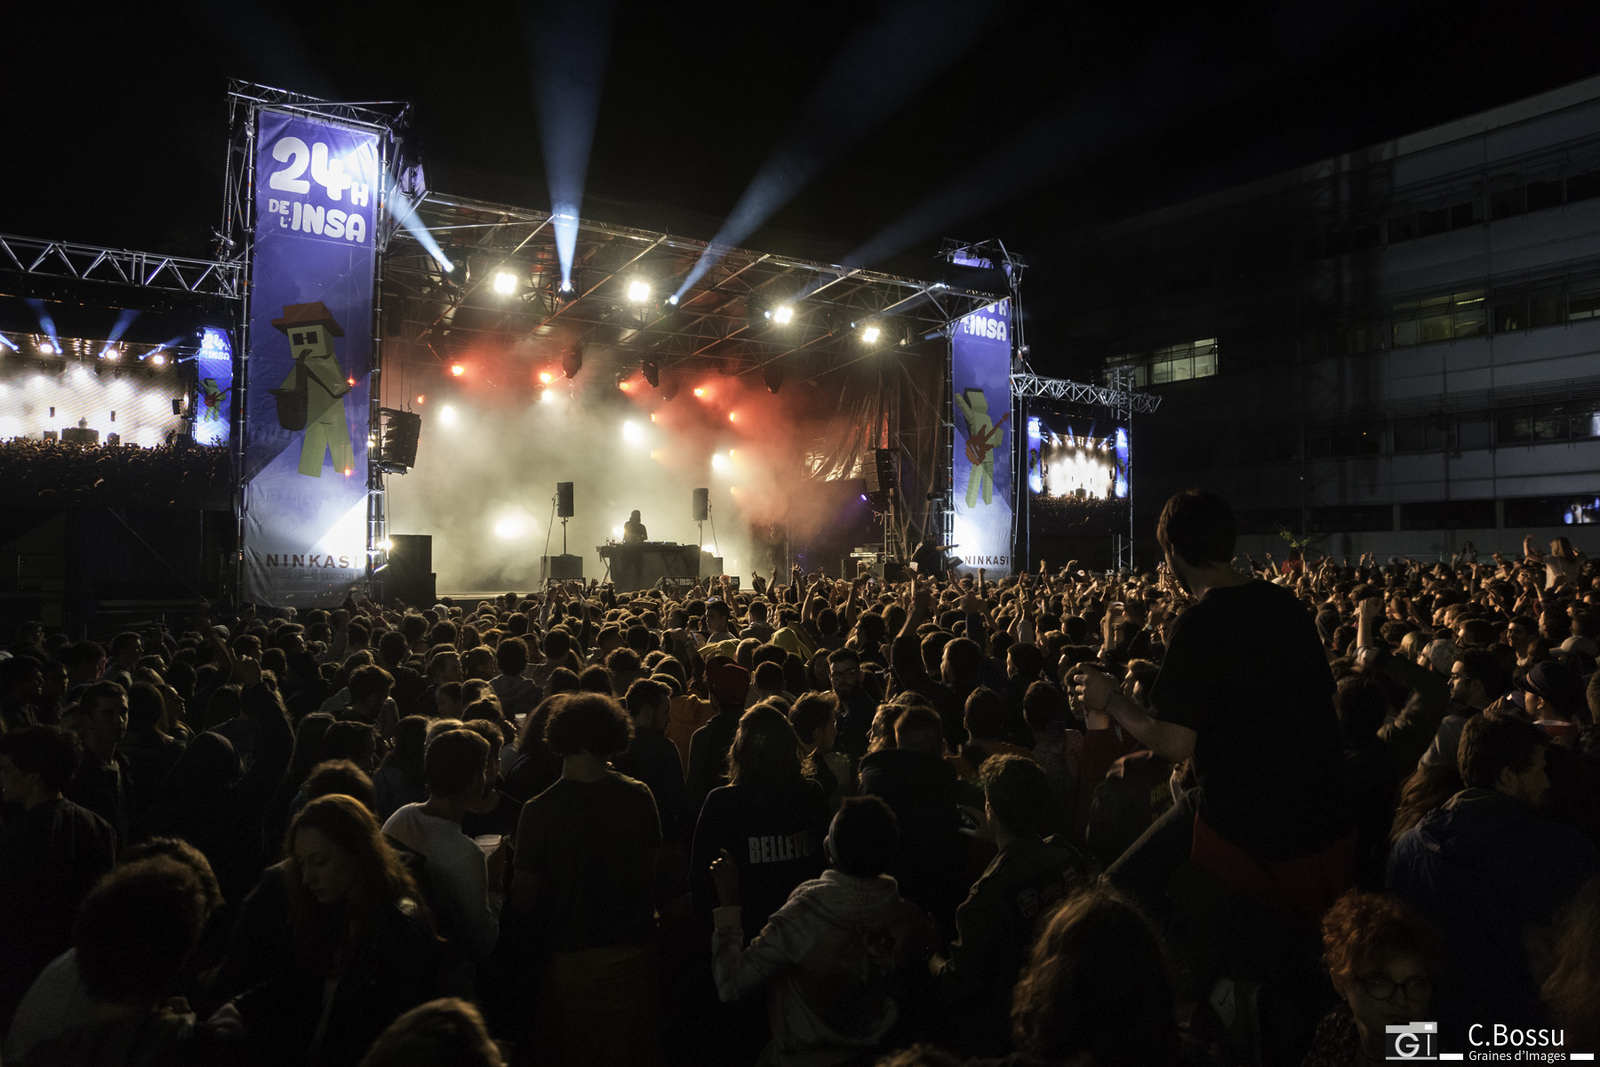
\includegraphics[width=.45\textwidth, trim=0 0 0 0,clip]{Images/Image5}}
\ParallelRText{\centering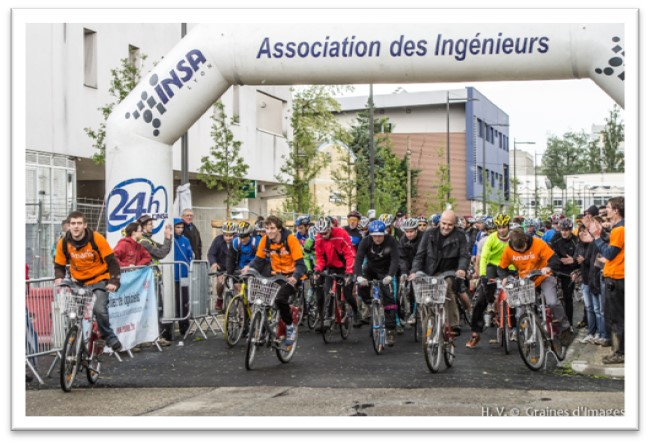
\includegraphics[width=.45\textwidth, trim=0 0 0 0,clip]{Images/Image6}}
\end{Parallel}

\end{frame}

\end{document}
